\documentclass[12pt,oneside]{book}
\usepackage[english]{babel}
\usepackage[utf8]{inputenc}
\usepackage{amsmath}
\usepackage{graphicx}

\usepackage[colorinlistoftodos]{todonotes}
\usepackage{fullpage} % changes the margin
\usepackage[nottoc,notlof,notlot]{tocbibind}
\usepackage[
    backend=biber,
    style=numeric,
    natbib=true,
    sorting = none,
    url=false, 
    doi=true,
    eprint=false
]{biblatex}
\addbibresource{main.bib}
\usepackage{float}
\usepackage[titletoc]{appendix}
\usepackage{setspace}
\usepackage{pdfpages}
\usepackage{url}
\usepackage[bottom]{footmisc}
\usepackage{textcomp}
\usepackage{caption}
\usepackage{subcaption}
\usepackage{longtable}
\usepackage{wrapfig}
\usepackage{bigfoot}
\DeclareNewFootnote{default}
\usepackage{soul}
\usepackage{hyperref}
\hypersetup{colorlinks=True}
\graphicspath{ {images/} }
\usepackage{csquotes}
\setlength{\parindent}{30pt}
\setlength{\parskip}{0.5em}
\graphicspath{ {Images/} }
\newcommand\measurepage{\dimexpr\pagegoal-\pagetotal-\baselineskip\relax}
\usepackage{amsmath,amssymb}
\usepackage{bm}
\setcounter{tocdepth}{4}
\setcounter{secnumdepth}{4}
\usepackage{mathtools}
\DeclarePairedDelimiter\bra{\langle}{\rvert}
\DeclarePairedDelimiter\ket{\lvert}{\rangle}
\DeclarePairedDelimiterX\braket[2]{\langle}{\rangle}{#1 \delimsize\vert #2}

\begin{document}

\begin{titlepage}

\newcommand{\HRule}{\rule{\linewidth}{0.5mm}} 


\includegraphics[width = 40mm]{DQT_LOGO_cmyk_BIG__1_.png}%
\hfill

\includegraphics[width = 10cm]{University_College_London_logo_svg.png}



\vspace*{3cm} % Leave 3.5inches for logo at binding service

%----------------------------------------------------------------------------------------
%	HEADING SECTIONS
%----------------------------------------------------------------------------------------

\textsc{\large Submitted for the Degree of MRes. in Delivering Quantum Technologies 2018}\\[0.5cm] % Major heading such as course name

%----------------------------------------------------------------------------------------
%	TITLE SECTION
%----------------------------------------------------------------------------------------

\HRule \\[0.4cm]
\centering
{ \huge \bfseries Investigating strain effects in $^{171}$Ytterbium doped Y$_{2}$SiO$_{5}$}\\[0.5cm] % Title of your document
\HRule \\[1cm]
 
%----------------------------------------------------------------------------------------
%	AUTHOR AND SUPERVISOR SECTION
%----------------------------------------------------------------------------------------

\begin{minipage}{0.4\textwidth}
\begin{flushleft} \large
\emph{Author:}\\
Lindsey F. \textsc{Keary}\\[0.5cm] 
\emph{Registration Number:} \\
17099595 
\end{flushleft}
\end{minipage}
~
\begin{minipage}{0.4\textwidth}
\begin{flushright} \large
\emph{Supervisor:} \\
Prof. John J. L. \textsc{Morton} \\[0.5cm]
\end{flushright}
\end{minipage}\\[1cm]

%----------------------------------------------------------------------------------------
%	DISCLAIMER SECTION
%----------------------------------------------------------------------------------------

%Except where explicitly stated all the work in this report, including appendices, is my own and was carried out during my final year. It has not been submitted for assessment in any other context.\\[0.25cm]
%I agree to this material being made available in whole or in part to benefit the education of future students.\\

%----------------------------------------------------------------------------------------
%	SIGNATURE SECTION
%----------------------------------------------------------------------------------------

%\vfill % Force the signature and date line to bottom of page

%Signature: \underline{\hspace{5cm}}\hfill
%Date: \underline{\hspace{5cm}}\hfill

\end{titlepage}

% \linespread{1.3} % Set the line spacing to 1.5
\spacing{1.2}

%----------------------------------------------------------------------------------------
%	FRONT MATTER
%----------------------------------------------------------------------------------------

\frontmatter

	\chapter{Abstract} The aim of this research is to gain insight into the effect of strain on rare-earth (RE) ions doped in Yttrium Orthosilicate (YSO) by applying unaxial strain to the crystallographic axes. This spin system has exciting potential for future hybrid quantum devices due to accessible optical and microwave transitions. Therefore there is significant interest in coupling RE doped YSO to superconducting qubits or resonators. Therefore, the strain mechanisms arising at the interface between the systems due to rate of material compression at cryogenic temperatures may perturb the bulk properties of the spins. Therefore, gaining a better understanding of the systems response to strain could better guide device fabrication. In addition similar experimental investigations of donor spins in silicon (Si) has provided useful information regarding the shift in spin Hamiltonian coupling terms.     


  	\chapter{Acknowledgments} Firstly, thank to my supervisor Prof John Morton for the opportunity to complete this project, for his support, his expert knowledge and for welcoming me into the quantum spin dynamics group during the 10 week project. I would like to also thank Prof Andrew Fisher for his involvement in guiding the theoretical treatment of this project, for insightful discussions and for good book recommendations. I would like to thank all present members of the quantum spin dynamics group for providing a friendly working environment in the shared laboratories.  

A special thank you is due to Gavin Dold and Pierandrea Conti for their involvement overseeing all aspects of this project. I thank Gavin for his kindness, patience, advise and willingness to answer any queries. In addition his direction to obtain to crucial simulations and for leading the re-installment of Zoidberg. I would like to thank Pierandrea for ensuring fabrication requiring the use of the machines at the Institute of Making was completed before the closure and for directing further fabrication. Also, I appreciate the long hours you accompanied me in the laboratory during the short available time to complete experimental measurements, for your willingness answer questions and enthusiasm to teach me to operate the equipment. 

Lastly, I would like to warmly thank CDT cohort 4 for their friendship and support throughout this year. The time spent sharing laughs, beer and lots of vegan food lifted the workload and dispelled any feeling of loneliness whilst living in London. I will greatly miss not seeing everyone of you every day. 



    \chapter{Thesis Outline}
\label{ch:Outline}
Below is a description of this thesis outline.
\par
\par
\noindent \textbf{Chapter 1:}{\addtolength{\leftskip}{5 mm} provides a brief introduction to quantum computing followed by a review of recent experimental achievements relating to RE doped YSO and its potential to provide the memory and micro-to-optical conversion in a hybrid quantum computing architecture. Additionally, the applications and investigation of strain effects observed in a hybrid devices when superconducting resonators interface with spin systems are considered. \\*

}

\noindent \textbf{Chapter 2:} {\addtolength{\leftskip}{5 mm}
Section~\ref{sec:electronparamagneticresonance} provides an introduction to electron paramagnetic resonance (EPR) and the spin Hamiltonian. In particular pulsed-ESR is described using the magnetisation vector picture as a semi-classical analogy of a spin-1/2 particle's evolution on the Bloch sphere in the presence of a driving field. In Section~\ref{sec:YSO} the crystalline structure of yttrium orthosilicate (YSO) is presented, followed by an introduction to the electronic structure of rare-earth doped ions. Lastly in Section~\ref{sec:YSO} the properties specific to $^{171}$Yb$^{3+}$ doped YSO are discussed. 
Section~\ref{sec:strain} presents the mathematical relationship between stress and strain. In addition the stiffness matrix components for YSO with derivation of the transformation to conventional dielectric axes is presented. \\*


}

\noindent \textbf{Chapter 3:} {\addtolength{\leftskip}{5 mm} This chapter details the experimental methods relevant for the investigation of strain in rare-earth doped YSO. Section~\ref{sec:EPRexperimentsetup} describes the experimental setup required to complete EPR spectroscopy. Details of the operation of the sample cooling, resonator and spectrometer are presented. Furthermore, fabrication of the sample holders specific to each orientation of the Yb doped YSO sample is given in this section. The simulations completed using the MATLAB toolbox EasySpin are presented in Section~\ref{sec:simulation}. These simulations provide a guide to the orientation of the crystal based on the resonance magnetic field obtained and additionally provide primary investigation of the response to strain for this anisotropic system. \\*


}

\noindent \textbf{Chapter 4:} {\addtolength{\leftskip}{5 mm} Experimental results obtained using EPR spectroscopy and consideration of the effect of applying uniaxial stress to the crystal. \\*


}
\noindent \textbf{Chapter 5:} {\addtolength{\leftskip}{5 mm} This chapter summarises and discusses the results obtained for this project. Additionally possible routes of future work are presented. \\*


}



   

  	\tableofcontents
    
    \listoffigures
 
	\listoftables

%----------------------------------------------------------------------------------------
%	MAIN MATTER
%----------------------------------------------------------------------------------------

\mainmatter

	\chapter{\label{sec:casestudy}Literature Review}
\section{Introduction to Quantum Computing}
In a society where the development of technology has greatly impacted our lives it is interesting to think that not so long ago, in 1936, the idea of a computer or a "Turing machine" was an abstract concept devised by Alan Turing~\citep{Turing1937OnEntscheidungsproblem,Nielsen2010QuantumInformation}. The basic idea of the machine is is an infinite tape of cells and a tip head moves along the tape with the ability to modifying and read out the cell contents. Therefore for any problem by programming a series of instructions to the machine can simulate the outcome. Many problems are efficiently solvable using a deterministic Turing machine. However, complexity classes were devised as a way to assess the difficulty of a problem based on the resources, space or time, required for simulation. For $\bm{P}$ problems the solution can be gained in polynomial time, which means time is a polynomial function of the size of input bits, n. However, there are a range of algorithms where the computational time required scales exponentially and means as $n$ increases the computation quickly becomes impracticable~\citep{talbot_welsh_2006}.

Furthermore, the field of quantum mechanics was born in 1900 following Planck's solution to the spectral energy density of blackbody radiation~\citep{Maxplanck}. This lead to the idea of quantisation where Einstein proposed the idea of energy quanta and postulated that energy is absorbed or emitted in discrete amounts~\citep{doi:10.1002/andp.19053220607}. This idea was verified by the famous photoelectric effect experiment~\citep{0143-0807-32-4-018}. In the years following applications and experimental studies of quantum mechanics theory grew, particularly following the development of the maser~\citep{PhysRev.99.1264}. Additionally, the development of the transistor in 1958 lead to the first integrated circuit which was the revolutionized the study of computer science ~\citep{Arns1998TheTransistor}. 

Moore's prediction of the population increase by reduction in the transistor size has held correct for the past 30 years~\citep{Moore1965CramingCircuits}. However, continuing to increase computational power by the scaling down the transducer size is reaching the fundamental limit where quantum effects of electrons dominate circuit operation. Investigation of algorithms to efficiently solve problems that are outwidth $\bm{P}$-space lead to the classification of the bounded error, quantum, polynomial time (BQP) complexity class. BQP includes all problems which are solvable using a quantum computer. Computational power is increased $\bm{(1)}:$ due to the ability to store information in a superposition of bit states, $\epsilon \left \{ 0,1 \right \}$ known as a qubit: 

\begin{equation}
\label{eq:qubit}
\ket{\Psi} = \alpha \ket{0} + \beta \ket{1},  
\end{equation} 

\noindent where $\alpha, \beta$ are complex probability amplitudes, and $\bm{(2)}:$ the ability to entangle qubits ~\citep{Nielsen2010QuantumInformation}. For example the factorization problem Shor's algorithm~\citep{doi:10.1137/S0097539795293172} computes the result in polynomial time and Grover's search algorithm provides quadratic speed up compared to classical computation~\citep{Grover:1996:FQM:237814.237866}. Additionally, in 1982 Feynman first introduced the idea that to simulate quantum behaviour, this required a universal computer which is also quantum in nature~\citep{Feynman1982}. 

In the pursuit to build a quantum computer the system to provide the basic quantum unit, satisfying the DiVencenzo criteria~\citep{Divincenzo2000TheComputation}, is an active area of research. There is a large variety of systems being investigated including: atoms, ions, photons, superconducting circuits (SC), quantum dots and atomic impurity spins in solids ~\citep{0034-4885-74-10-104401,10.1038/nature07129,MORTON2018128}.   
  


\section{Prospects of Rare-earth Doped YSO for Quantum Computing}
Distributed quantum computing is the scheme were a large scale quantum computer is sectioned into nodes connected via optical channels~\citep{DiVincenzo255}. The separation of quantum nodes is limited by light attenuation for distribution $>$100 km and the no-cloning theorem which prevents classical amplification of entangled photons~\citep{Duan2001Long-distanceOptics}. This principle naturally leads to the hybrid quantum computing approach where disparate qubits are used to their individual advantage to form either local processors or memory qubits in each node~\citep{nature07127}. Scalable solid state devices such as SC circuits, SC resonators~\citep{Houck2009} and donor electron spins in doped solids \citep{doi:10.1146/annurev-conmatphys-062910-140514} provide fast (ns) gate manipulation and microwave regime readout. These systems provide promising candidates to provide processor qubits. Conversely, their ability to store information is limited by their short ($\mu$s) coherence times. Thus it is advantageous for memory qubits to also provide coherent microwave-to-optical conversion as means of interfacing photonic and solid state qubits. Currently quantum repeaters systems are focused on cavity QED approaches where the memory qubit is provided by: NV centers in diamond~\citep{PhysRevA.92.020301}, Rydberg atoms~\citep{PhysRevA.96.013833} or rare-earth (RE) doped crystals~\citep{PhysRevB.84.060501}. Details of the crystal structure and energy level splitting of RE doped YSO is detailed in Section.~\ref{sec:YSO}.  

Replacing yttrium atoms with RE ions results in small inhomogeneous broadening of the microwave and optical transitions. Thus RE doped YSO presents a promising platform for hybrid quantum computing where the host lattice has a low nuclear spin abundance~\citep{PhysRevB.97.064409}. The demonstration of a coherence time of 370 minutes for the nuclear spin of $^{151}$Eu doped Y$_{2}$SiO$_{5}$~\citep{nature14025} at 2 K motivates the study of RE ions for coherent quantum information storage applications. This system provides the longest measured coherence time of a quantum memory system with optically accessible transitions. This result is achieved by a reduction in the decoherence of the +3/2 $\leftrightarrow$ -3/2 hyperfine transitions firstly reducing the sensitivity to fluctuations of the magnetic field $\bm{B_{0}}$, reducing the spin-reconfiguration rate and lastly the inclusion of the KDD$_{x}$ pulse sequence. Due to the zero-field splitting of hyperfine states, operation at the zero first-order Zeeman (ZEFOZ) magnetic field produces hyperfine clock transitions the expected ideal decoherence rate is 2.9$\time 10^{-2}$ s$^{-1}$. 

A significantly smaller decoherence rate is observed for the case where the pulse separation time  $\tau$ of the Hahn echo sequence is considerably shorter than the phase memory time, $T_{M}$~\citep{PhysRev.168.370}. The "froze core" effect~\citep{PhysRevB.91.214303} reduces the spin flipping rate of the Yttrium nuclear spins around an Eu ion due the hyperfine interaction with the magnetic moment of the unpaired electron in a large magnetic field as shown in Fig.~\ref{fig:frozencore}. The nuclear dipolar interaction resulting in a fluctuating magnetic field is therefore reduced~\citep{RevModPhys.79.1217}. Further extension of the spin coherence time was successfully achieved using the KDD$_{x}$ pulse sequence. This sequence provides dynamical decoupling from the environment to provide protection from the environmental induced dephasing using a series of refocusing pulses~\citep{PhysRevLett.106.240501}. 

\begin{figure}[h]
\centering
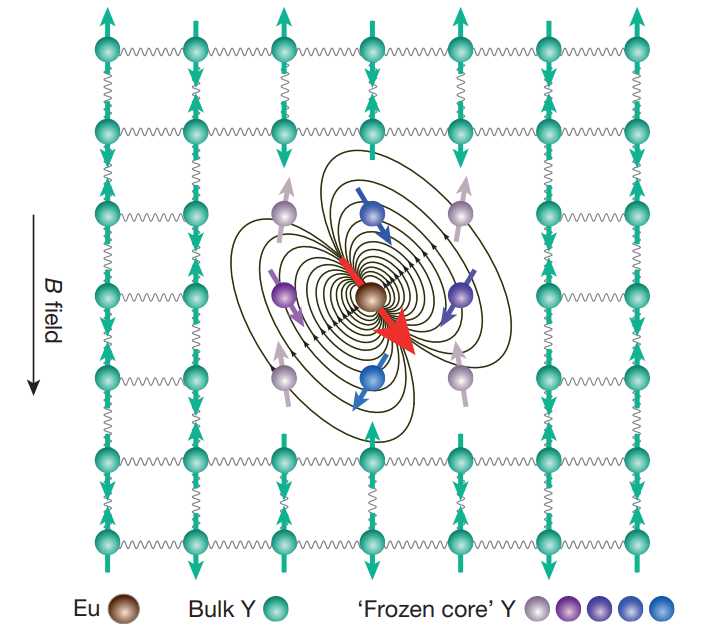
\includegraphics[height=0.32\textwidth,keepaspectratio]{frozencore}
\caption{\label{fig:frozencore} The "frozen core" effect where the large electron dipole moment (red arrow) of the Eu ion induced by an external magnetic field modifies the Larmor frequency of Yttrium spin procession such that Yttrium ions in the frozen core cannot swap spin with the bulk Yttrium nuclei ~\citep{nature14025}.}
\end{figure}


Including microwave electron paramagnetic resonant transitions, RE ions have near infra-red optical transitions~\citep{PhysRevB.94.155116}. Therefore, the active research investigates the ability to couple RE doped crystals to SC resonators. Strong coupling is achieved between SC niobium chip and Er$^{3+}$ doped Y$_{2}$SiO$_{5}$ has been achieved~\citep{PhysRevLett.110.157001}. The SC device contains 9 $\approx$50 GHz element resonators which is connected by glue to two RE doped crystals. This system is sometimes referred to as a "flip chip". Due to the highly anisotropic nature of RE ions in YSO the g-tensor depends on the angular orientation of $\bm{B_{0}}$ with respect to the x-axis is given as:

\begin{equation}
\label{eq:qubit}
g(\phi) = \sqrt{g_{y}^{2}cos^{2}(\phi)+g_{z}sin^{2}(\phi)},  
\end{equation}

\noindent where $g_{y}$ and $g_{z}$ are two of the three principle values. Therefore the coupling strength between the Er$^{3+}$ electron spins and the SC resonator AC microwave driving field, $\bm{B_{1}}\cos(\omega t)$, is a function of g-tensor elements: 

\begin{equation}
\label{eq:qubit}
\nu_{1} \propto \frac{g_{y}g_{z}\left | B_{1} \right |}{g(\phi)}.  
\end{equation}

Thus the largest coupling is achieved when AC field is aligned along the largest component of the g-tensor, which for this crystal is the along $g_{z} = 14.8$. However, to achieve strong coupling condition $\eta > 1$ must be satisfied where $\eta =4\nu^{2}/\kappa \Gamma$~\citep{TANJISUZUKI2011201}. Therefore, the broadening of the transition linewidth $\Gamma$ as function of the $g(\phi)$ is also an important consideration. Thus strong coupling is achieved for 12 MHz linewidth transition with g = 1.4 with $B_{0}$=100 mT .     


An alternative scalable hybrid system investigated is fabricating a NbN resonator on top of a sapphire substrate implanted with RE Gd$^{3+}$ ions~\citep{doi:10.1063/1.4894455}. The sapphire substrate provides a low dielectric loss and natural impurity system. Investigation of the enhanced coupling, $\nu'=\nu \sqrt{N}$, through using a controlled ion implantation technique to dope the substrate with $N$ spins. Good agreement is obtained between the numerical modeling of $\nu$ based on the concentration distribution of implanted ions and the experimental result. Despite the strong coupling regime not yet having been reached, thin film deposition directly onto the crystal surface is a promising approach. The reduction of the number interfaces reduces dielectric loss and this hybrid architecture may be applicable for RE doped YSO. 

Moreover, multimode storage and retrieval of a quantum state is an important function required for a hybrid quantum computing scheme~\citep{Kurizki3866}. Coherent storage and retrieval of a microwave field was first achieved using collective spin coupling of $\approx$10$^12$ NV centers to a SC resonator~\citep{PhysRevA.92.020301}. The storage and retrieval cycle between the resonator and the spin system has a period of $\pi / \nu'$ and tuning of the resonator is implemented by changing the flux through the SQUID loop. The output microwave pulse amplitude $A(t)$ is measured as a function of the pulse duration $\tau$ where the $ns$ decay rate of the signal compared to the spin energy damping rate of $\approx$1 second is due to inhomogeneous broadening effects since the experiment is not yet operating in the strong coupling regime. The addition of a transmon qubit enables storage of superposition qubits states through electrostatic qubit-SC resonator and magnetic resonator-spin ensemble coupling~\citep{PhysRevLett.107.220501}. In Ref.~\citep{PhysRevA.92.020301} using a Hahn echo pulse to refocus the NV spins, retrieval of a low power microwave pulse resulting in a single photon in the resonator is implemented.

\begin{figure}[h]
\centering
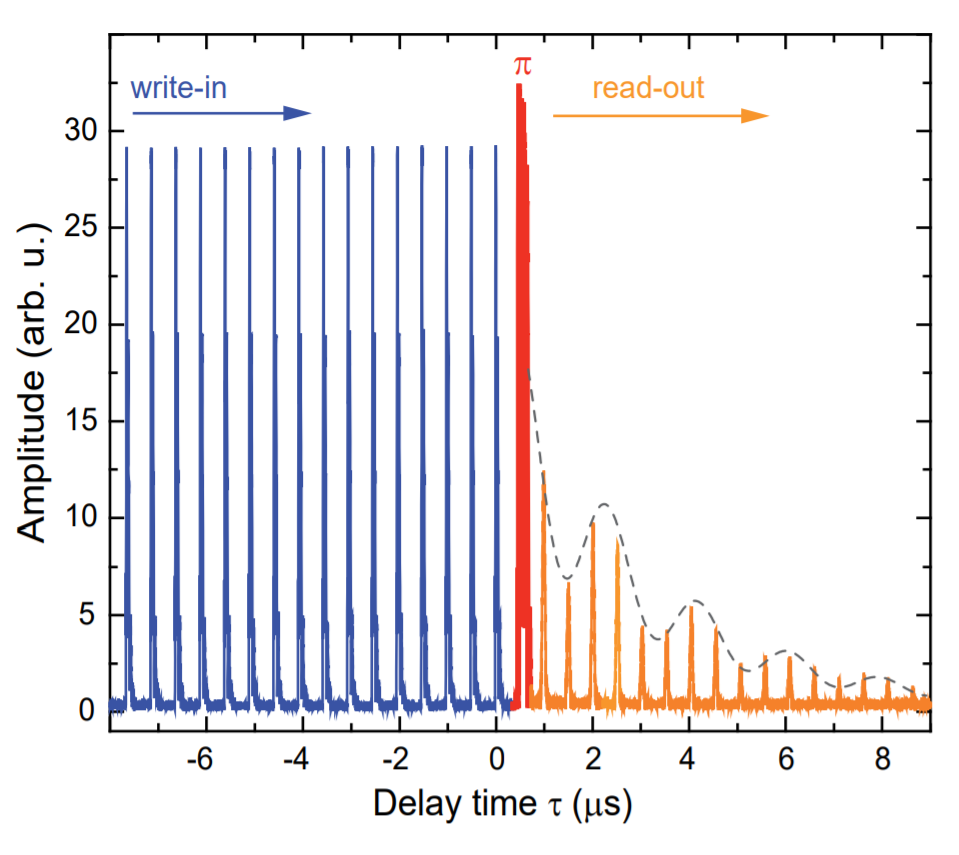
\includegraphics[height=0.4\textwidth,keepaspectratio]{16state}
\caption{\label{fig:16state} Storage of 16 microwave coherent pulses in the high field $S_{2a}$ electronic transition of Eu ions. The grey dashed line is the electron spin echo envelope modulation due to the hyperfine interaction between Y nuclear spins and Eu electronic spins \citep{PhysRevB.92.014421}.}
\end{figure}

Multimode storage and retrieval of 16 weak coherent microwave pulses in a Er$^{3+}$ doped YSO crystal placed on a copper coplanar waveguide is demonstrated at $mK$ temperature in Ref.~\citep{PhysRevB.92.014421}. Collective ensemble encoding for a spin system due to the absorption of a photon is described as:

\begin{equation}
\label{eq:qubit}
\ket{\Psi}_{c} = \frac{1}{\sqrt{N}} \sum_{k=1}^{N}\ket{\downarrow_{1} \downarrow_{2}...\uparrow_{k}...\downarrow_{N}}\exp{-i\delta_{k}t}, 
\end{equation} 

where $\delta_{k}$ is the k-th spin detuning from the average precession frequency of the spin ensemble. Dephasing results in $\ket{\Psi}_{c}$ evolving into a dark mode. Thus another single photon can be absorbed by spins. The number of stored modes, which is 56 for this system, is upper-bounded by $T_{2}/T_{2}^{*}$ where $T_{2}$ is the coherence time and $T_{2}^{*}$ is the dephasing time. The application of the refocusing $\pi$-pulse results in the emission of the microwave pulses is shown in Fig.~\ref{fig:16state} where the output photon emission is reversed with respect to the input photons. The oscillatory behavior of the retrieved pulses is expected to be due to the nuclear spin of Y ions interacting with the RE electronic spins. This additionally indicates that nuclear spin of $^{89}$Y ions has potential for memory applications. In addition, reversible mapping of temporal optical modes using Nd doped YSO with a 883 nm transition wavelength is investigated in Ref.~\citep{Usmani2010MappingMP}. 


\begin{figure}[h]
\centering
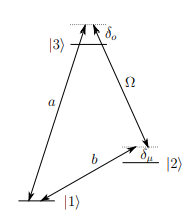
\includegraphics[height=0.4\textwidth,keepaspectratio]{3levelatom}
\caption{\label{fig:3levelatom} Energy level schematic of the Er atoms. The microwave cavity mode is coupled to the spin transition with frequency $\omega_{b}$. The optical cavity mode couples to the $\ket{1}\leftrightarrow \ket{3}$ transition with frequency $\omega_{a}$. There is an additional coherent driving field $\Omega$ for the transition $\ket{2}\leftrightarrow \ket{3}$ ~\citep{PhysRevLett.113.203601}.}
\end{figure}


Reversible mapping of multimode pulses in RE doped substrates is an impressive step towards building a hybrid quantum memory. Conversely, the distributed quantum computing architecture additionally requires the ability to achieve efficient microwave-to-optical conversion to enable long distance transmission of quantum states. In Ref.~\citep{PhysRevLett.113.203601} a theoretical proposal for a 100$\%$ efficient microwave-optical transducer is outlined for a cryogenic Er doped crystal. The crystal is placed inside a microwave and optical resonator where coupling of the Er atoms to the cavities is described in Fig.~\ref{fig:3levelatom}. The three off-resonant fields are detuned such that $\omega_{a} = \omega_{b}+\omega_{\Omega}$. The photons emitted by Er occur at a wavelength compatible with long distance transfer over an optical fiber. For large detuning such that excited atomic states are adiabatically eliminated the Hamiltonian terms describing the coupling between the two modes has a strength, S:

\begin{equation}
\label{eq:qubit}
S = \sum_{k} \frac{\Omega_{k}\nu_{\mu,k} \nu^{*}_{o,k}}{\delta_{o,k}\delta_{\mu,k}}
\end{equation}

where the coupling strengths of $k$-th atom to the microwave and optical resonator is $\nu_{\mu,k}$ and $\nu_{o,k}$ respectively. The coherent driving field has the Rabi frequency $\Omega_{k}$. Therefore to achieve perfect mapping of the microwave field to an optical field the condition $4\left | S \right | = \kappa_{a}\kappa_{b}$ must be satisfied where $\kappa$ describes the cavity decay rate. Thus efficient conversion requires coupling between the Er atoms and one or both of cavities to be in the strong coupling regime. Strong coupling of RE ions to a microwave cavity has been achieved in Ref.~\citep{PhysRevLett.110.157001} as previously discussed and strong coupling to an optical cavity is demonstrated in Ref.~\citep{PhysRevA.74.033818}.      

\begin{figure}[h]
\centering
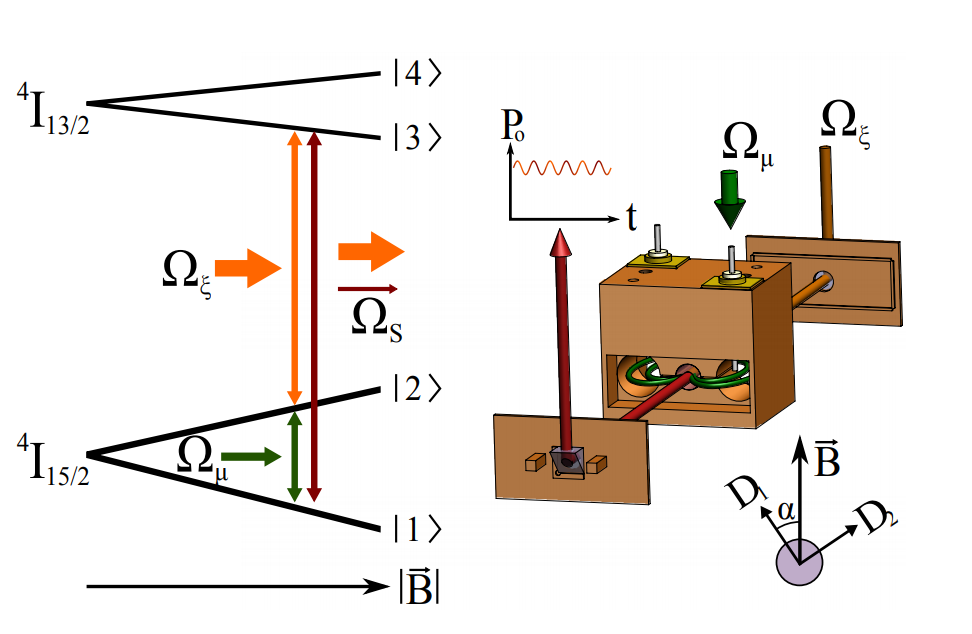
\includegraphics[height=0.4\textwidth,keepaspectratio]{frequencyupconversion}
\caption{\label{fig:frequencyupconversion} (Left) The optical transition is obtained between the $^{4}$I$_{15/2}$ and $^{4}$I$_{13/2}$ energy levels of Er doped YSO which is driven by the $\Omega_{\xi}$. The application an external field magnetic field results in the $^{4}$I$_{15/2}$ electron spin resonance being driven by the $\Omega_{\mu}$ field. The resulting optical field is $\Omega_{s}$. (Right) The experimental schematic where the sample resides inside the loop-gap resonator where the dielectric axis of the crystal with respect to input microwave fields is shown. Light is transmitted to or from the sample using via a prism pair ~\citep{PhysRevA.92.062313}.}
\end{figure}

Experimental demonstration of microwave-to-optical conversion using an Er doped YSO sample is presented in Ref.~\citep{PhysRevA.92.062313}. The experimental setup and coupling transitions are shown in Fig.~\ref{fig:frequencyupconversion}. The input microwave and optical field generate a coherence between $\ket{1} \rightarrow \ket{3}$ where using the Raman heterodyne spectroscopy scheme, the output of this field is detected through the beat note of the optical coupling beam. The low efficiency of the conversion is expected to be improved by the addition of an optical resonator to increase the coupling strength.  

To summarise recent investigations of RE doped YSO illustrates the exciting potential of this system to provide a quantum memory of a hybrid distributed quantum computing architecture. The experimental schemes discussed here highlight that RE ions can achieve strong coupling to microwave and optical cavities which is a crucial requirement for a quantum transducer protocols. Additionally storage and retrieval of multimode microwave pulses is an initial impressive step towards building a quantum memory, where the ultimate goal is reversible, high-efficiency quantum state transfer between disparate qubits.



\section{The effect of strain in hybrid quantum systems}
The motivation for this project arises due to the interest in coupling RE doped YSO to superconducting resonators using the flip-chip approach~\citep{PhysRevLett.110.157001} or direct metal deposition~\citep{doi:10.1063/1.4894455}. The requirement of cryogenic temperatures for operation is expected to induce strain in the crystal environment. This effect is due to difference in thermal expansion coefficients for the substrates and thus could produce a perturbation of the spin distribution. Similarly, this a concern for donor spins in silicon where superconducting resonators are patterned onto the sample~\citep{doi:10.1063/1.4919761}. 

The expected cause of the observed variation from the bulk properties for nano-fabricated electronic substrates on donor spin doped Si substrates was due to induced electric fields or strain effects~\citep{10.1038/NNANO.2014.211}. Investigation of resonance shifts of three aluminum superconducting resonators pattered on the surface of a 700 nm isotropically purified $^{28}$Si substrate with implanted $^{209}$Bi donors~\citep{PhysRevApplied.9.044014}.Electron paramagnetic resonance (EPR) spectroscopy completed on the $\ket{F=4,m_{F}=-4} \leftrightarrow \ket{F=5,m_{F}=-5}$ transition, where $\Delta m_{F} = \pm 1$. This reveals transition peak splitting each with a 100 $\mu$T linewidth compared to single 20 $\mu$ peak measured in the absence of a patterned superconducting resonator as shown in Fig.~\ref{fig:straininducedsplitting}. 


\begin{figure}[h]
\centering
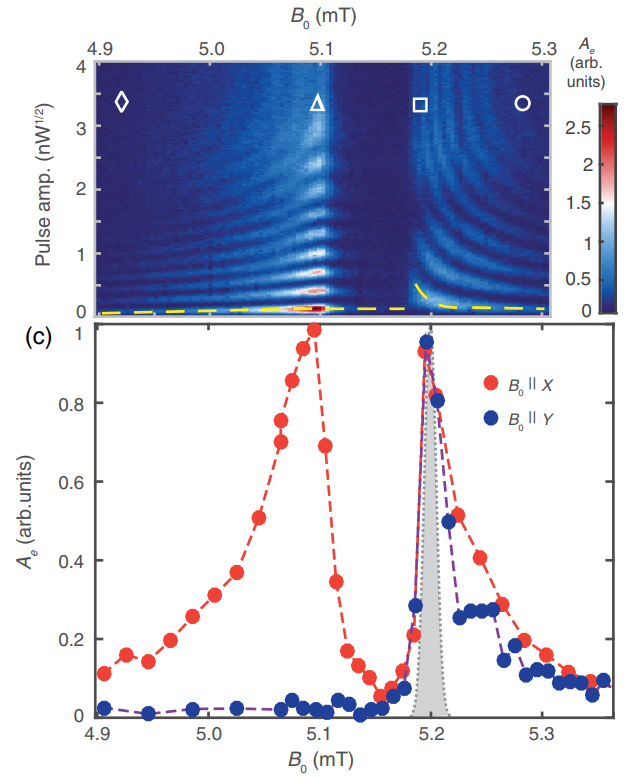
\includegraphics[height=0.45\textwidth,keepaspectratio]{straininducedsplitting}
\caption{\label{fig:straininducedsplitting} The echo signal detected using the Hahn echo sequence for the $\ket{F=4,m_{F}=-4} \leftrightarrow \ket{F=5,m_{F}=-5}$ for $B_{0} \parallel X$ (red) and $B_{0} \parallel Y$ (blue). The grey curve shows the peak transition for the system with no on-chip resonator ~\citep{PhysRevApplied.9.044014}.}
\end{figure}


The low peak observed for  vanishes for $B_{0} \parallel X$ vanishes for $B_{0} \parallel Y$ which is attributed to the condition $\delta B_{1}\perp B_{0}$ for excitation, where $\delta B_{1}$ is the magnetic field vacuum fluctuations in the resonator. Directly under an electrode, of the interdigited LC resonator, dominated by $\delta B_{1Y}$ with contribution of $\delta B_{1Z}$ to the side of the electrode. Therefore, only $\delta B_{1z}$ contributes for $B_{0} \parallel Y$. Further investigation of spin transitions discounts an in-built electric field or magnetic field inhomogeneity as the mechanism for the splitting and broadening of the transition peak. Therefore upon consideration of strain, this mechanism has the ability to modify the electron spin (S=1/2) and nuclear spin (I=9/2) transitions for $^{209}$Bi. Strain can modify the quadrupole interaction, the hyperfine interaction strength $A$ and the electron g-factor.   

The quadrupole interaction arises due to axial symmetry of the nuclear charge distribution where nuclear quadrupole moment $Q$ describes the degree of deformation from spherical charge distribution. The non-spherical nucleus interact with nearby electrons resulting in an electrostatic field gradient $V_{ab}$ at the nucleus where $a$ and $b$ are the local crystal frame principle axes. The Hamiltonian term for the quadrupole interaction is thus:

\begin{equation}
\label{eq:quadropleinteraction}
H_{Q} = \frac{e V_{zz} Q}{4I(2I-1)}\left [3I^{2}_{z}-I^{2}+\eta (I^{2}_{x} - I^{2}_{y} \right ],
\end{equation} 

where the asymmetry parameter is $\eta = (V_{xx}-V_{yy}/V{zz}$ and the electron charge is $e$~\citep{Suits2006}. Ref.~\citep{PhysRevLett.115.057601} demonstrates that the quadrupole interaction can be manipulated by strain applied to Si doped with As$^{+}$ ions using piezo-actuators. The induced strain can be used to tune the nuclear spin properties of As$^{+}$ ions. For the unstrained sample the cubic crystal symmetry cancels out the electric field gradients whilst applying uniaxial strain mimics the effect of strain induced at mK temperatures for substrates with different thermal expansion coefficients and results in a nonzero electric field gradient. 

\begin{figure}[H]
    \centering
    \begin{subfigure}[b]{0.6\textwidth}
        \centering
        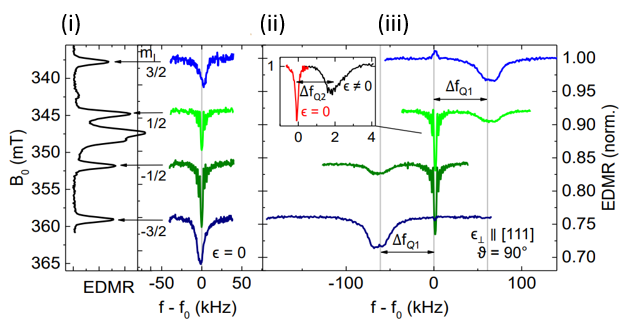
\includegraphics[width=\textwidth]{nuclearshifts}
        \caption{\label{fig:nuclearshifts}(i) electrically detected
magnetic resonance (EDMR) spectrum for As$^{0}$ in Si. (ii) unstrained NMR transitions for As$^{+}$ in Si. (iii) strained NMR transitions for A$^{+}$. The insert shows the $\ket{m_{I}=1/2} \leftrightarrow \ket{-1/2} $ transitions in high-resolution~\citep{PhysRevLett.115.057601}.}
    \end{subfigure}
        \begin{subfigure}[b]{0.6\textwidth}
        \centering
        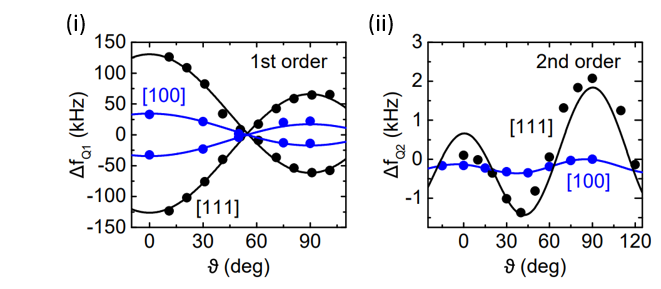
\includegraphics[width=\textwidth]{nuclearshifts2}
        \caption{\label{fig:nuclearshifts2} Angular dependence of (i) first-order and (ii) second-order resonance frequency shifts dependent on the magnetic field orientation where the electric field gradient generated in [111] and [100] crystal directions~\citep{PhysRevLett.115.057601}.}
    \end{subfigure}
    \caption{}
\label{fig:}
\end{figure}

Comparison of the unaxial strain of the order of 10$^{-4}$ and unstrained nuclear magnetic resonance (NMR) spectrum probed using 9.74 GHz resonator is shown in Fig.~\ref{fig:nuclearshifts}. This reveals outer transitions (ie $\ket{m_{I}=3/2} \leftrightarrow \ket{1/2}$ and $\ket{-3/2} \leftrightarrow \ket{-1/2}$ have a resonance shift greater than the resonance linewidth described by the first order frequency shift. Additionally for these transitions asymmetric broadening is observed in absence of the piezo-mechanical strain and is attributed to strain induced by the contact. Conversely only a small second order frequency shift is observed for the sharp $\ket{1/2} \leftrightarrow \ket{-1/2}$ resonance. Further investigation using long rf-pulses as shown in the insert of Fig.~\ref{fig:nuclearshifts} determines that the inner transition is similarly shifted by more than one linewidth but due to the difference in linewidth, between the inner and outer transition, the shift is significantly smaller. Fig.~\ref{fig:nuclearshifts2} presents a characterisation of the resonance shift due to anisotropic electric field gradient as a function of angle $\vartheta$ between magnetic field and strain axis. The quadrupole shift is related to the applied strain through the a tensor $S_{ij}$ with nonzero $S_{11}$ and $S_{44}$ components. However, comparison of $df/dQ$ sensitivity to EPR transitions it is clear the quadrupole interaction is not the origin of the resonance splitting~\citep{PhysRevApplied.9.044014}.

The study of strain induced resonance frequency shifts due to perturbation of the hyperfine coupling of group V donor spins in $^{28}$Si is completed~\citep{PhysRevLett.120.167701}. The compressive strain is applied using masses placed on top of the sample and is expected to modify the band structure of Si. Thus the valley repopulation model (VRM)~\citep{PhysRev.124.1068} was utilised to understand the effect of Si crystal symmetry breaking which lifts the Si six valley degeneracy. Strain induces mixing of the donor singlet $A_{1}$ ground state and the doublet $E$ excited state. The hyperfine interaction Hamiltonian term is presented in Section.~\ref{sec:hyperfine} where the isotropic hyperfine interaction strength $A$ is given in Eq.~\ref{eq:hyperfinestrength}. The EPR transitions of $^{209}$Bi doped in Si, the sample mount and observed shift in resonance frequency due to small (10$^{-5}$) strain is shown in Fig.~\ref{fig:mansirpaper}. 

\begin{figure}[h]
\centering
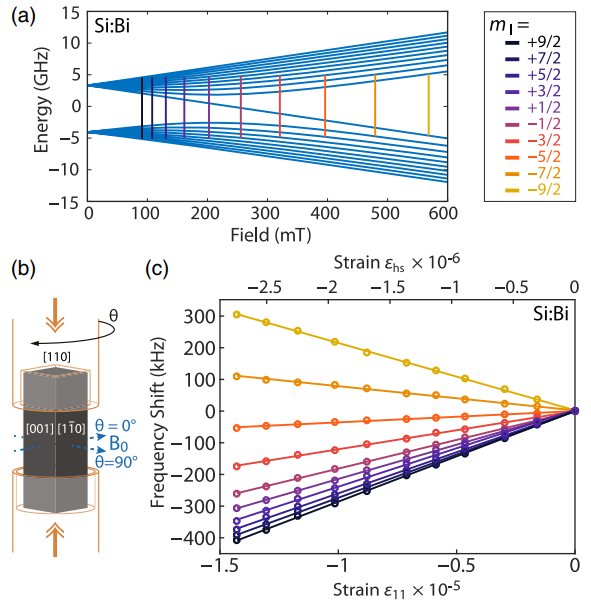
\includegraphics[height=0.45\textwidth,keepaspectratio]{mansirpaper}
\caption{\label{fig:mansirpaper} (a) $^{209}$Bi (S=1/2, I=9/2) doped in Si EPR spectrum. (b) Mechanical strian experimental setup where $\theta$ is orientation of $B_{0}$ with respect to the [001] crystal axis. (c) Observed linear EPR frequency shifts as a function of the strain $\epsilon_{11}$ for $\theta = 30^{\circ}$ ~\citep{PhysRevLett.120.167701}.}
\end{figure}

The VRM model predicts quadratic shift of $A$ for the application of unaxial strain. However, the observed linear shift is attributed to uniaxial stress applied to the crystal producing three linear strain components, $\epsilon_{11}$, $\epsilon_{22}$ and $\epsilon_{33}$ where the hydrostatic strain mechanism is described as $\epsilon_{hs} = (\epsilon_{11}+\epsilon_{22}+\epsilon_{33}/2$). Comparison of isotropic hyperfine coupling $df/dA$ to the experimentally measured $df/d\epsilon_{11}$ determines the linear strain mechanism dominates. The tight binding (TB) model~\citep{PhysRevB.79.245201} describing the variation of bound states $Bi$ doped Si under strain provides a good agreement for small applied strain with experimentally. The determined relationship $A/A_{0}$ where $A_{0}$ is the unstrained hyperfine interaction strength to second order the strain is:

\begin{equation}
\label{eq:Atermmodel}
A(\bm{\epsilon})/A_{0} = 1+\frac{K}{3}(\epsilon_{xx}+\epsilon_{yy}+\epsilon_{zz})+\frac{L}{2}\left [ (\epsilon_{yy}-epsilon_{zz})^{2}+(\epsilon_{xx}-\epsilon_{zz})^{2}+(\epsilon_{xx}-\epsilon_{yy})^{2}) \right ] +N(\epsilon^{2}_{yz}+\epsilon^{2}_{xz}+\epsilon^{2}_{xy}),
\end{equation} 

where A fit to the TB model obtains K = 29.3, L = -9064 and N = -225. Additionally, investigation the induced anisotropy of the g-tensor for V group donors in Si is fitted to a model developed which contains a VRM term and the spin-orbit coupling term. Applying the model in Eq.~\ref{eq:Atermmodel} to the Si doped As$^{+}$ device with LC resonator pattered on the surface in Ref.~\citep{PhysRevApplied.9.044014} determines $A(\bm{\epsilon})=$ 1MHz for strain of the order of 10$^{-4}$. This results in a resonance shift in agreement with the experimentally measured result of Fig.~\ref{fig:straininducedsplitting}. Therefore the strain induced modification of the $A$ is determined to be the resonance peak splitting mechanism. 


\begin{figure}[h]
\centering
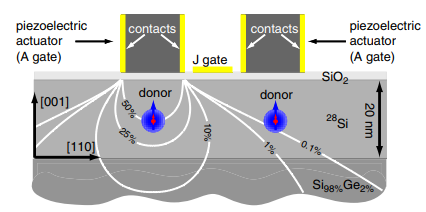
\includegraphics[height=0.45\textwidth,keepaspectratio]{piezoelectric}
\caption{\label{fig:piezoelectric} The schematic of the piezoelectric actuators which can apply strain to the $^{28}$Si substrate in locations of a donor spin. This device tunes the coupling strength between the nuclear and electronic spin of the P donor. The distribution of the out of plane strain is illustrated using isolines is modelled using density function theory calculations. To maximise the effect of the nanoactuators $^{28}$Si is grown on a SiGe substrate ~\citep{PhysRevLett.106.037601}.}
\end{figure}

The applications of the strain induced ability to shift a resonance peak of a spin system by more than a linewidth does not go unnoticed \citep{PhysRevLett.120.167701,PhysRevApplied.9.044014,PhysRevLett.115.057601}. The scheme to Stark tune the hyperfine interaction of P doped Si using piezoelectric nanoactuators is illustrated in Fig.~\ref{fig:piezoelectric}. This scheme provides a 17 $\mu$T shift of the P hyperfine transitions with a 8 $\mu$T linewidth. Therefore, this device has potential to provide an additional degree of freedom to tune qubits in and out of resonance. Additionally, in Ref.~\citep{PhysRevB.88.064308} applying mechanical stress to a single acceptor in a patterned Si substrate is shown to partially lift the ground state degeneracy. In the presence of strain in addition to the magnetic field the qubit can decoupled to the first order decoupled from the acoustic phonons used to coherently manipulate the state of the qubit.   

The theoretical treatment of the interaction between the applied strain and electron spin of NV centers is presented in Ref.~\citep{PhysRevB.98.075201}. This study suggests that magnetically forbidden transitions, in addition to allowed transition, can be coherently driven using mechanically deforming the crystal at a rate equal to the Rabi frequency. In Ref.~\citep{PhysRevLett.111.227602} the ground state Hamiltonian of the spin system is given as:

\begin{equation}
\label{eq:HamiltonianNV}
H_{NV} = D_{0}S^{2}_{z}+\gamma_{NV}B_{\parallel}S_{z}+\gamma_{NV}B_{\perp}S_{x}+\epsilon_{\perp} \left | \sigma_{x}(S_{x}S_{y}+S_{y}S_{x})+\sigma_{y}(S^{2}_{x}-S^{2}_{y}) \right |, 
\end{equation} 

where $D_{0}$ and $\gamma_{NV}$ is the zero-field splitting and the gyromagnetic ratio, respectively. The degeneracy of the $\ket{m_{s}=0}$ and $\ket{\pm 1}$ is lift by $D_{0}$. The components of the magnetic field are given as $B_{\parallel}$ and $B_{\perp}$ and the components of the electron spin operator as $S_{x},S_{y} and S_{z}$ where z-axis is along the crystal's symmetry axis. Alignment of $B_{\parallel}$ splits the degeneracy of $\ket{+1}$ and $\ket{-1}$. Coherent driving of $\ket{0} \leftrightarrow \ket{\pm 1}$ is achieved by an oscillating $B_{\perp}$ field. The addition of a GHz stress perpendicular to the symmetry axis drives the magnetically forbidden spin transition $\ket{-1} \leftrightarrow \ket{+1}$. Thus addition of mechanical strain enables driving between all the spin states. A bulk acoustic resonator is used to generate the stress resonant with the $\ket{-1} \leftrightarrow \ket{+1}$ transition where the magnetic spin resonance is achieved using an optical detection scheme at room temperature. Moreover, in Ref.~\citep{2040-8986-19-4-044003} decoupling from the environmental noise is achieved by driving the spin transitions with a mechanical oscillator. The coherence time of the qubit is increased by two orders of magnitude.  
    

    \chapter{Theory}

\section{\label{sec:electronparamagneticresonance}Electron Paramagnetic Resonance}
Electron paramagnetic resonance (EPR) is a sensitive spectroscopy technique used in to characterise systems. This technique can be used to determine information about the electronic structure since the measured parameters can be related to the electronic wavefuction for systems which have an unpaired electron and thus are paramagnetic~\citep{}. 

EPR gives information about the electronic structure since magnetic paramters are related to the electronic wavefunction and the configuration of surrounding nuclei with nonzero spins. 
Following the demonstration of quantised orientations of an atom's electron magnetic momentum $\hbar \textbf{S}$ in an applied magnetic field by Stern and Gerlach in 1922~\citep{10.1007/BF01326983}, Ulenback and Goudsmit related the angular momentum of an electron to the magnetic moment $\bm{\mu}$ ~\citep{10.1007/BF01558878}. The first EPR resonance was measured in a sample of CuCl$_{2}\cdot$H$_{2}$O in 1945 by Zavoisky using a 133 MHz frequency and 4.76 mT field. 


This method is akin to nuclear magnetic resonance (NMR) where the nonzero atomic nuclear spin, however in EPR spectroscopy it is the nonzero electron spin which results in degenerate states. ESR experiments are completed at low temperatures where the atomic energy splitting is large enough such that it is typically only the ground state's response to perturbations is considered whilst the excited states only indirectly influence this behavior~\citep{Stoneham}. 

The principle of NMR lead to the significant medical application referred to as magnetic resonance imaging (MRI). The medical applications of ESR are less well established but this spectroscopy tool shows promise to provide measurement of $O_{2}$ in living tissue which has uses in oximetry and radiation dosimetry \citep{10.1039/c1pc90002a}. More generally, physics and chemistry applications result from the ability to probe molecules with an unpaired electron using this sensing technique. In quantum technologies pulsed EPR experiments are used extensively on spin systems to obtain information such as the spin relaxation time, $T_{1}$ and effective dephasing time, $T_{2}^{\star}$.

This technique has applications in the study of defect and impurity crystals \citep{Stoneham}. The paramagnetism of rare earth ions is from an unpaired electron in 4f shell where the atomic structure of the rare-earth ion Y$_{b}$ is discussed in greater detail in Section.\ref{}. In the case of this experiment, ESR will be utilised to detect the shift in frequency of the rare-earth dopant resulting from perturbations of the $\bm{g}$ and $\bm{A}$ tensors of the spin Hamiltonian for this system. Further context and detail is provided in the following sections. 

\subsection{\label{sec:zeeman}The Zeeman Interaction}
The term in the spin Hamiltonian which has a dependence on the magnetic field is known as the Zeeman interaction Hamiltonian, $\hat{H}_{Z}$. This term describes the interaction between the electron/nuclear spin with the applied static magnetic field $\bm{B}_{0}$ along the z-axis:

\begin{equation}
\label{eq:zeemanhamiltonian}
\hat{H}_{Z}=-\bm{B_{0}}\cdot \bm{\hat{\mu}}=-B_{0} (\hat{\mu}_{ez}+\hat{\mu}_{nz}).
\end{equation} 

\noindent The electron and nucleus magnetic moment operators are given as $\hat{\mu}_{ez}$ and $\hat{\mu}_{nz}$, respectively. The magnetic moment of spin particles arises due to the spin angular momentum~\citep{atherton1973electron}: 

\begin{minipage}{0.4\linewidth}  
\begin{equation}
\label{eq:electronspinoperator}
\hat{\mu}_{ez}= -g \mathcal{B}_{e} \hat{S}_{z},
\end{equation}  
\end{minipage}  
\hspace{0.5cm}  
\begin{minipage}{0.4\linewidth}  
\begin{equation}
\label{eq:nuclearspinoperator}
\hat{\mu}_{nz}= -g_{n} \mathcal{B}_{n} \hat{I}_{z},
\end{equation}  
\end{minipage}

\noindent where $\hat{S}_{z}$ is the electron-spin operator and $\hat{I}_{z}$ is the nuclear-spin operator projected along the $z$-axis. 

The Bohr and nuclear magnetons are expanded as:

\begin{minipage}{0.4\linewidth}  
\begin{equation}
\label{eq:electronspinoperator}
\mathcal{B}_{e} = \frac{e\hbar}{2m_{e}},
\end{equation}  
\end{minipage}  
\hspace{0.5cm}  
\begin{minipage}{0.4\linewidth}  
\begin{equation}
\label{eq:nuclearspinoperator}
\mathcal{B}_{n} = \frac{e\hbar}{2m_{p}},
\end{equation}  
\end{minipage}

\noindent where $m_{e}= 9.11 \times 10^{-31}$ kg is the mass of an electron and $m_{p}=1.673 \times 10^{-27}$ kg is the mass of a proton. The significantly larger electron mass and thus larger $\mathcal{B}_{e}$ compared to $\mathcal{B}_{n}$ results in the external magnetic field more strongly coupling to the unpaired electron \citep{weil1994electron}. Therefore, in quantum information processing each particle has a different advantages. Electron spin qubits have fast gate manipulation but the sensitivity to magnetic field noise limits the coherence time ~\cite{10.1038/nature11449}. Alternatively, the weak interaction of the nuclear spin with its environment lead to the qubit memory applications for this type of spin qubit~\citep{nature12011}. 

The Zeeman Hamiltonian can be written in full as given in Eq.~\ref{eq:fullzeemanhamiltonian}. 


\begin{equation}
\label{eq:fullzeemanhamiltonian}
\hat{H}_{Z}=\textbf{B}^{T}\frac{1}{\hbar} \left (\mathcal{B}_{e}\textbf{g}\hat{\textbf{S}}-\mathcal{B}_{e} g_{n}\hat{\textbf{I}}\right )
\end{equation} 

The real and symmetric second-rank $\textbf{g}$ tensor for anisotropic systems describes the energy dependence with the orientation of $\hat{\textbf{S}}$ relative to $\textbf{B}$. However, the g factor in Eq.~\ref{eq:electronspinoperator} is the effective value average over all orientations. The $\textbf{g}$ tensor is often represented as a diagonal matrix in the molecular frame using the principle values, $g_{x}$, $g_{y}$ and $g_{z}$ where any rotation from the principle frame is described using Euler angles. For an isotropic system $g_{x}=g_{y}=g_{z}$. Anisotropy of $\bm{g}$ arises when system lacks symmetry resulting in an energy dependence with the $\hat{\bm{S}}$ orientation with respect to $\bm{B_{0}}$. The nuclear $g_{n}$ factor is an intrinsic property of the nucleus and the minimal contribution of $\bm{g_{n}}$ is generally considered to be isotropic~\citep{schweiger2001principles}. 

In the simplest EPR example, the electron spin quantum number $S=\frac{1}{2}$ and the nuclear spin quantum number $I=0$. In this case the solution to Eq.~\ref{eq:fullzeemanhamiltonian} provides the energy eigenvalues: 

\begin{equation}
\label{eq:fullzeemanhamiltonian}
U = \pm g \mathcal{B}_{e}B.
\end{equation} 

The magnetic quantum states $m_{s} = \pm \frac{1}{2}$ are shown below in Fig.~\ref{fig:hyperfinenergylevelsplitting} where their separation is varied by changing the applied magnetic field $\bm{B_{0}}$. The center frequency, $\nu \approx 9$ GHz of an additional radio-frequency (rf) oscillating magnetic field $\bm{B_{1}}$ is resonant when $\Delta U=h\nu$. 

\begin{figure}[h]
\centering
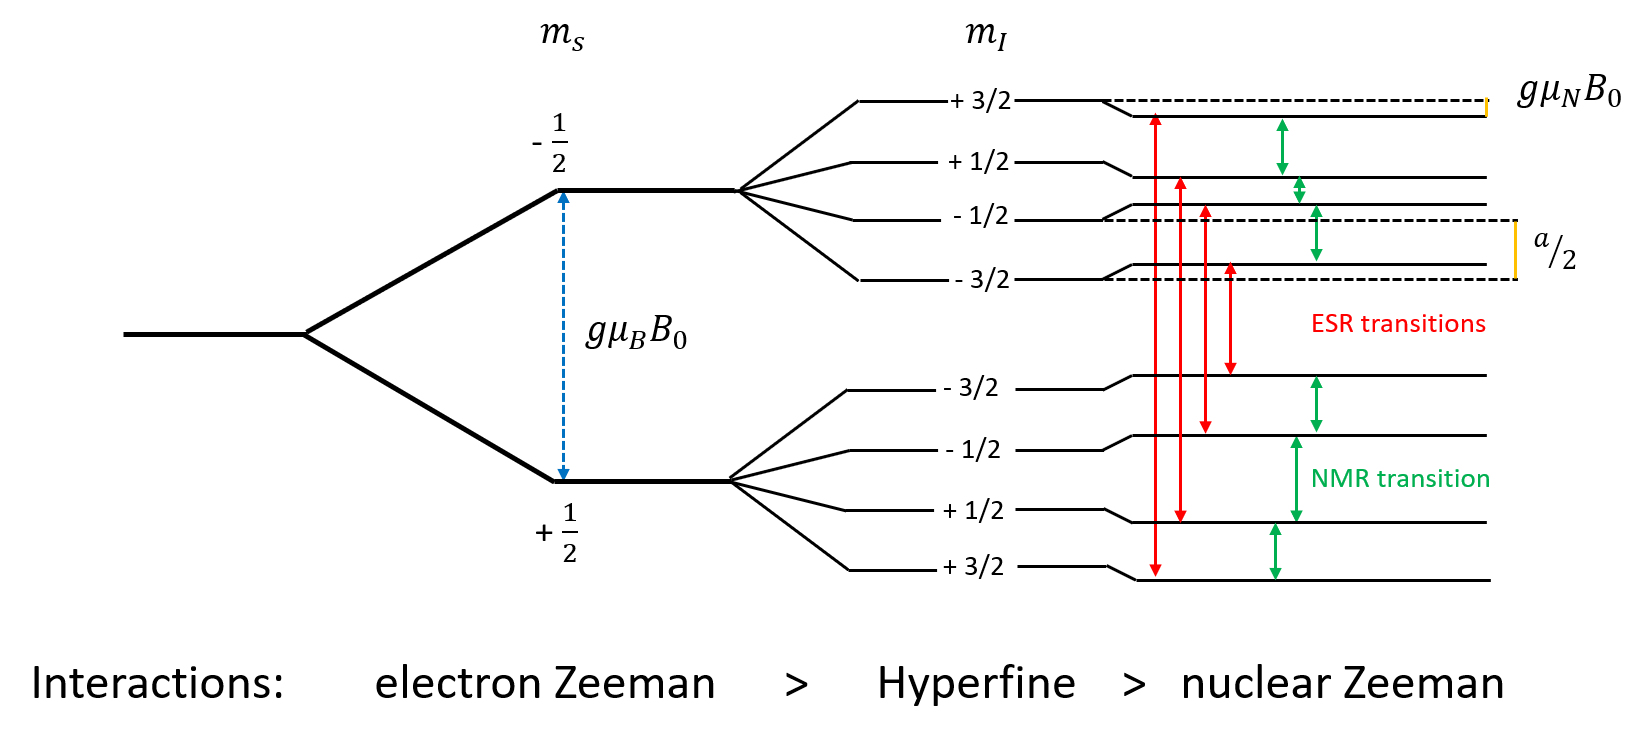
\includegraphics[height=0.32\textwidth,keepaspectratio]{hyperfinenergylevelsplitting}
\caption{\label{fig:hyperfinenergylevelsplitting} Example of an energy level diagram for a system where $S=1/2$ and $I=1/2$. The electron and nuclear Zeeman interactions terms are shown. Additionally the hyperfine interaction level splitting is shown.}
\end{figure}




%SUBSECTION HYPERFINE
\subsection{\label{sec:hyperfine}The Hyperfine Interaction}
NRI experiments can be used to probe the nuclear Zeeman splitting for spin systems where $I \neq 0$. However, there is a more significant detectable degeneracy shown in Fig.~\ref{fig:hyperfinenergylevelsplitting} which arises due to the hyperfine interaction. The hyperfine Hamiltonian term is given below as: 

\begin{equation}
\label{eq:fullzeemanhamiltonian}
\hat{H}_{HF}=\hat{\bm{S}}^{T} \bm{A} \hat{\bm{I}}
\end{equation} 

\noindent which describes the interaction between the electron and nuclear spin operators. The symmetric second-rank $\bm{A}$ tensor describes the hyperfine coupling. For an isotropic system the coupling constant is given as:

\begin{equation}
\label{eq:hyperfinestrength}
A_{o} = \frac{2\mu_{o}}{3} g\mathcal{B}_{e} g_{n}\mathcal {B}_{n}|\psi (0)|^{2} 
\end{equation} 

\noindent which gives a measure of the magnetic interaction energy between the spin particles. The electron spin density at the nucleus is given by $|\psi (0)|^{2}$.

However, if $\bm{A}$ anisotropic results in changes in the energy level splitting dependent on the orientation of the sample. The hyperfine anisotropy arises due the electron and nuclear dipole interaction. Classically this interaction energy is described by Eq.\ref{eq:classicaldipolarenergy} where $r$ is the separation distance between the unpaired electron and nucleus.


\begin{equation}
\label{eq:classicaldipolarenergy}
U_{dipolar}(\bm{r}) = \frac{\mu_{o}}{4 \pi}\left [ \frac{\bm{\mu_{e}}^{T}\cdot \bm{\mu_{n}}}{r^{3}}-\frac{3(\bm{\mu_{e}}^{T}\cdot \bm{r})(\bm{\mu_{n}}^{T}\cdot \bm{r})}{r^{5}}\right ]
\end{equation} 

\noindent $\bm{\mu_{e}}$ and $\bm{\mu_{n}}$ are the magnetic moment for the electron and nucleus, respectively. Therefore transforming to the quantum-mechanical description the Hamiltonian describing the anisotropic hyperfine interaction is:

\begin{equation}
\label{eq:quantumdipolarenergy}
\hat{H}_{dipolar}(\bm{r}) = \frac{\mu_{o}}{4 \pi} g \mathcal{B}_{n} g_{n} \mathcal{B}_{n} \left [ \frac{\hat{\bm{S}}^{T} \cdot \hat{\bm{I}}}{r^{3}}-\frac{3(\hat{\bm{S}}^{T} \cdot \bm{r} )(\hat{\bm{I}}^{T} \cdot \bm{r})}{r^{5}} \right ],
\end{equation}

\noindent which simplifies to Eq.~\ref{eq:quantumdipolarham} following integration over the electron distribution in the crystal. 

\begin{equation}
\label{eq:quantumdipolarham}
\hat{H}_{dipolar} = \hat{\bm{S}}^{T} \cdot \bm{T} \cdot \hat{\bm{I}} 
\end{equation}

\noindent Therefore the hyperfine coupling tensor is given as $\bm{A} = A_{o}\bm{\mathcal{I}_{3}} + \bm{T}$. 







%SUBSECTION PULSED EPR 
\subsection{Pulsed EPR}
\subsubsection{The Magnetisation Vector Picture}
In this section the magnetisation vector picture is used to introduce an illustration of pulse EPR experiments. In Eq.~\ref{eq:electronspinoperator} the description of the magnetic moment for a single electron is given. For a sample containing $N$ unpaired electrons with individual magnetic moments align parallel to an applied magnetic field $\textbf{B}$ whilst $\textbf{S}$ aligns anti-parallel following from Eq.~\ref{eq:electronspinoperator} gives the minimum energy. The effective macroscopic moment is $\bm{\mu}=\sum_{i}^{N} \bm{\mu_{i}}$. Therefore measurements of the spin ensemble obtains the magnetisation of the sample is given as:


\begin{equation}
\label{eq:macroscopicmagnetisation}
\textbf{M}=\frac{1}{V}\sum_{i}^{N} \bm{\mu_{i}},
\end{equation} 

\noindent which is the net magnetic moment per unit volume, $V$. An individual magnetic moment experiences a torque when in presence of a magnetic field~\citep{schweiger2001principles}:

\begin{equation}
\label{eq:torque}
\hbar \frac{d \textbf{S}}{d t}=\bm{\mu} \times \textbf{B}(t)
\end{equation} 

\noindent Therefore the ensemble magnetisation in a constant stable field $\bm{B_{0}}$ is:
\begin{equation}
\label{eq:magnetisationderiv}
\frac{d\bm{M}}{dt} = \bm{M} \times \frac{-g \mathcal{B}_{e}}{\hbar}\bm{B_{0}}.
\end{equation} 

\noindent The procession of the $\bm{M}$ around $\bm{B_{0}}$ is given by the Larmor frequency: 

\begin{equation}
\label{eq:Larmorfrequency}
\omega_{L} = \frac{g \mathcal{B}_{e} B_{0}}{\hbar},
\end{equation} 

where similarly as before $\bm{B_{0}}$ is defined as being applied along the z-axis \citep{foot2005atomic}. This description is informative as it is analogous to the precession of a spin-$\frac{1}{2}$ quantum state precessing at a rate of $\omega_{L}$ around the Bloch sphere in presence in an external magnetic field $B_{0}\bm{\hat{z}}$. 
 
\begin{figure}[h]
\centering
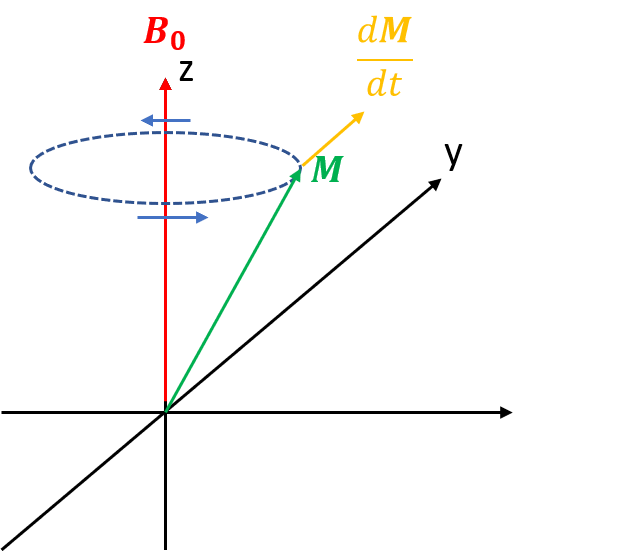
\includegraphics[height=0.32\textwidth,keepaspectratio]{magnetisationpicture}
\caption{\label{fig:magnetisationpicture} The Larmor precession of the magnetisation vector, $\bm{M}$ in the classical magnetisation vector picture.}
\end{figure}
 
 
In addition to a homogeneous magnetic field, transitions are driven between electron spin states via microwave pulses. Thus, the following provides the description of the inclusion of an oscillating magnetic field, $\bm{B_{1}}$ with a dependence on time. The components of $\bm{B_{1}}$ are:

\begin{equation}
\label{eq:magneticfieldcomponentsx}
B_{1x^{L}}(t) = B_{1}\cos(\omega_{MW}t),
\end{equation}
\begin{equation}
\label{eq:magneticfieldcomponentsy}
B_{1y^{L}}(t)=B_{1}\sin(\omega_{MW}t)
\end{equation}
\begin{equation}
\label{eq:magneticfieldcomponentsz}
B_{1z}(t) = 0.
\end{equation}
 
\noindent Following convention and describing system in the rotating frame where $\bm{B_{1}}$ is time-independent. Therefore the motion of the magnetisation in this frame is obtained by inserting $\bm{B} = \bm{B_{0}}+\bm{B_{1}}$ into Eq.~\ref{eq:magnetisationderiv}.There is an additional precession of frequency:

\begin{equation}
\label{eq:mwfieldirect}
\omega_{1}= \frac{g_{e}\mathcal{B}_{e} B_{1}}{\hbar},
\end{equation}

\noindent about the direction of $\bm{B_{1}}$.

The angle of the effective field the spins precess around is $\arctan(\omega_{1}/\Omega_{S})$ where $\Omega_{S} = \omega_{1}/\Omega_{S}$ where $\Omega_{S}= \omega_{L}-\omega_{MW}$. The spin precession rate is thus: 
\begin{equation}
\label{eq:mwfieldirecteffect}
\omega_{eff}=\sqrt{\Omega_{S}^{2}+\omega_{1}^{2}}.
\end{equation}

\noindent For the resonant case $\bm{M}$ is invariant. However, a large field effect occurs for small perturbations, where $\omega_{MW} \neq \omega_{L}$. It is now trivial to repeat the steps to calculate the effect of a linearly polarised microwave field perpendicular to $\bm{B_{0}}$, which is most likely the polarisation of the experimentally applied pulse. 




Therefore if a resonant microwave pulse is applied to the system for a time $t_{p}$ along the x-axis of the rotating frame, then magnetisation vector precessing around this axis is described as:

\begin{equation}
\label{eq:magneticfieldcomponentsx1}
M_{x}=0,
\end{equation}
\begin{equation}
\label{eq:magneticfieldcomponentsy1}
M_{y}=-M_{0}\sin(\omega_{1}t_{p}),
\end{equation}
\begin{equation}
\label{eq:magneticfieldcomponentsz1}
M_{z} = M_{0}\cos(\omega_{1}t_{p}),
\end{equation}

\noindent where for a spin system in thermal equilibrium initially $M_{0}=M_{z}$. Therefore rotation can be described by the $R_{x}(\omega_{1}t_{p})$ matrix. Therefore the rotation performed can be controlled by pulse duration, thus the combination of rotations enables rotation around a any desired axis~\citep{schweiger2001principles}.   




\subsubsection{Spin Manipulation} 
In this current picture it appears the magnetisation vector could precess for infinite amount of time around the Bloch sphere. However, this is not the case due to relaxation processes due to the interaction of a spin with it's environment. A single spin in the presence of an magnetic field will undergo longitudinal relaxation to it's thermal equilibrium state is due to stochastic processes such as phonon interactions, which is described in more detail in \label{sec:YSOdopedYbions}. In the magnetisation vector picture this relaxation mechanism is described as: 

\begin{equation}
\label{eq:mzfe}
M_{z}=M_{0}\left [ 1-2\exp{-\frac{t}{T1}} \right ],
\end{equation}

\noindent where $T_{1}$ is the decay time constant. Now considering a distribution of spin particles in the presence of $B_{0}$. Despite the aim to make $B_{0}$ completely homogeneous there will still remain a small degree of space anisotropy in the system. Therefore, the a distribution of spin will experience a slightly different $B_{0}$ field and thus will have slight different precession frequencies. This causes inhomogeneous broadening due to the frequency distribution. Spin relaxation due to inhomogeneous broadening is described by the time $T_{2}^{*}$.

The true decoherence time of the spin system is $T_{2}$ arises due to interaction of a spin with another spin which has been relaxed to the thermal equilibrium by a longitudinal relaxation mechanism. This produces the spin flip-floping process between the spins such that the upper bound of $T_{2}$:

\begin{equation}
\label{eq:T2upper}
T1 \leq 2T_{2}, 
\end{equation}

\noindent is dictated by $T_{1}$. In contrast for reversible dephasing $T_{2}^{*}$ time for the loss of quantum coherence can be refocused by applying the Hahn echo pulse sequence shown below in Fig.~\ref{fig:echopulsesequence}.

\begin{figure}[H]
    \centering
    \begin{subfigure}[b]{0.6\textwidth}
        \centering
        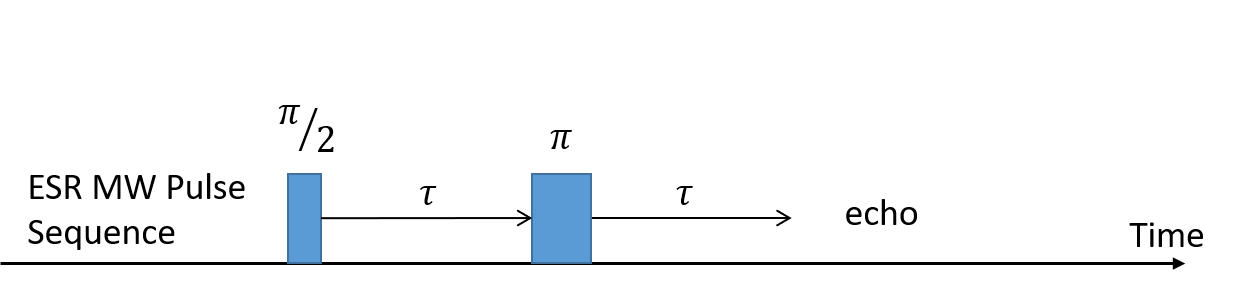
\includegraphics[width=\textwidth]{echopulsesequence}
        \caption{\label{fig:echopulsesequence}}
    \end{subfigure}
%     \hfill
    \begin{subfigure}[b]{0.6\textwidth}
        \centering
        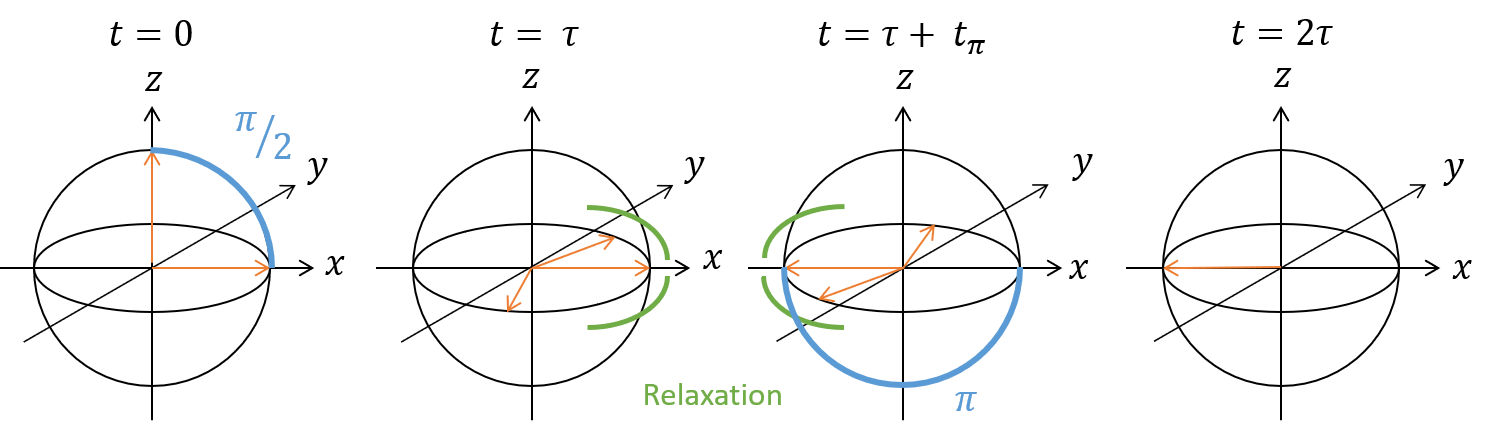
\includegraphics[width=\textwidth]{echoblochsphere}
   \caption{}
   \end{subfigure}
   \caption{(a) The Hahn echo pulse sequence. (b) Bloch sphere representation of the quantum state evolution resulting from the pulse sequence and spin dephasing.}
   \label{fig:blochsphererep}
\end{figure}

\noindent This sequence is used extensively in pulse-EPR schemes for signal detection. Additionally the inversion recovery sequence can be used to measure $T_{1}$. In this sequence shown in Fig.~\ref{fig:T1pulsesequence} an initial $\pi$-pulse is used to invert the spin state, followed by the Hahn echo pulse sequence where the time between the first $\pi$-pulse and the $\pi/2$ pulse is swept to obtain the longitudinal relaxation time. 



\begin{figure}[h]
\centering
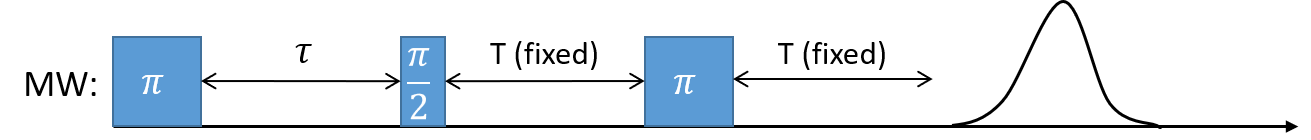
\includegraphics[height=0.05\textwidth,keepaspectratio]{T1pulsesequence}
\caption{\label{fig:T1pulsesequence} The inversion recovery pulse sequence.}
\end{figure}
 










% Recently single electron EPR held in a Penning trap. 
%v is the center frequency of the source of incident radiation

%The unitless g-factor g characterises the change in energy dependence on static magnetic
%field caused by the electron spin environment. 
%magnetic field to remove degeneracy


%schweiger:EPR gives information about the electronic structure since magnetic paramters are related to the electronic wavefunction and the configuration of surrounding nuclei with nonzero spins. 




    \section{\label{sec:YSO}{Rare earth doped Y$_{2}$SiO$_{5}$}}

\subsection{YSO Crystal Structure}
Yttrium Orthosilicate is a monoclinic crystal with with Si$^{4+}$ tetrahedral and lanthanide Y$^{3+}$ octahedral site symmetry \citep{SHOUDU1999901}. The Czochralski-growth technique for rare earth orthosilicates is detailed in Ref.~\citep{MELCHER19931001}. Depending on the growth temperature there are two possible monoclinic crystal structures which can form (X1 or X2). The Y$^{+3}$ ions can be substituted by activator rare earth ions. There are two inequivalent Y$^{+3}$ atomic sites with low C1 point symmetry for either crystal phase commonly referred to as site I and site II \citep{doi:10.1021/jp5050207}. The sites have a different volume due to the proximity of oxygen atoms. Therefore RE ions with radii larger than the Y$^{3+}$ radii (0.892 $\AA$) preferentially occupy the site I~\citep{nikl2016nanocomposite}.     

\begin{figure}[h]
\centering
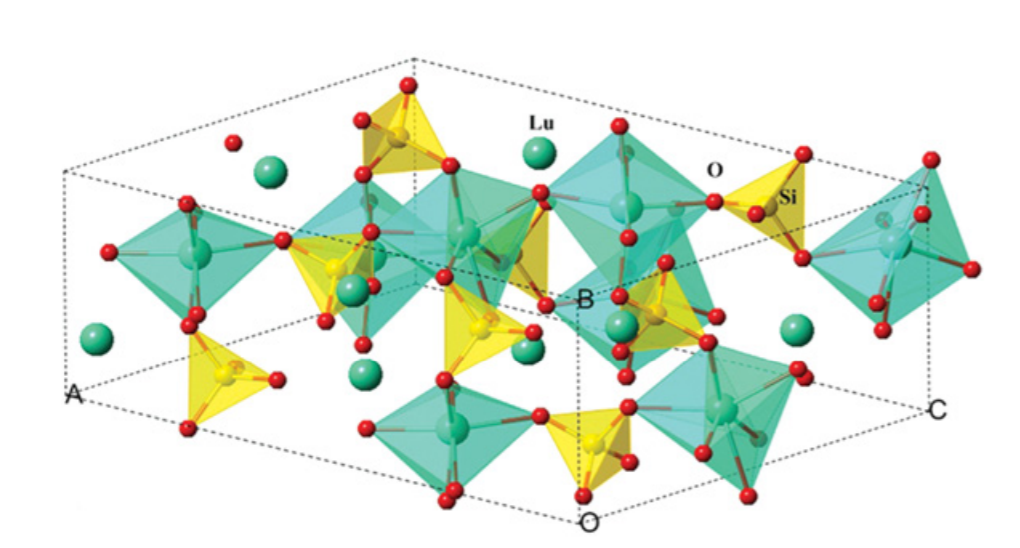
\includegraphics[height=0.32\textwidth,keepaspectratio]{YSOstructure}
\caption{\label{fig:YSOstructure} RE$_{2}$SiO$5$ crystal structure \citep{Ceramics}.}
\end{figure}


The space group of YSO is C$^{6}_{2h}$ with two-fold symmetry of the crystallographic $b$ axis (see Section.~\ref{sec: YSO stiffness matrix}). Therefore each site has two sub-sites which are related through 180$^{\circ}$ crystal rotation. The sub-sites are equivalent only when an applied magnetic field is parallel or perpendicular to the b-axis~\citep{PhysRevB.97.064409}. In addition to the nonorthogonal crystallographic axes, a monoclinic biaxial crystal has a set of orthogonal dielectric axes ($D1,D2,D3$) due to the three principle refractive indices. The b-axis is parallel to the $D3$-axis. The $D1$ and $D2$ axis are measured by placing the crystal between a crossed polarizer and applying a laser parallel to the $b$-axis. Rotation of the crystal perpendicular to the laser identifies the dielectric axes as no light is transmitted when $D1$ or $D2$ are collinear to the polarizers \citep{Traum:14}.     

%Therefore, the crystal is cut along the dielectric frame (D1,D2,b).

 
\subsection{Electronic Structure of Rare-earth Ions}


Rare earth elements are a group containing lanthenides, Scandium and Yttrium. In the 1950's P.P. Feofilov was one of the first physicists to investigate the optical spectroscopy of rare-earth activated crystals for applications in quantum electronics~\citep{MALKIN198713}. He observed diverse spectra dependent on the preparation method of the host material. The name rare earths is a misnomer as they are actually rather abundant in the Earth's core. However, the issue is extracting RE ions as mining of a single element is not possible. These elements exist in ores contain many different metals, with extremely similar chemical properties~\citep{benelli2015introduction}.  
   

\begin{figure}[h]
\centering
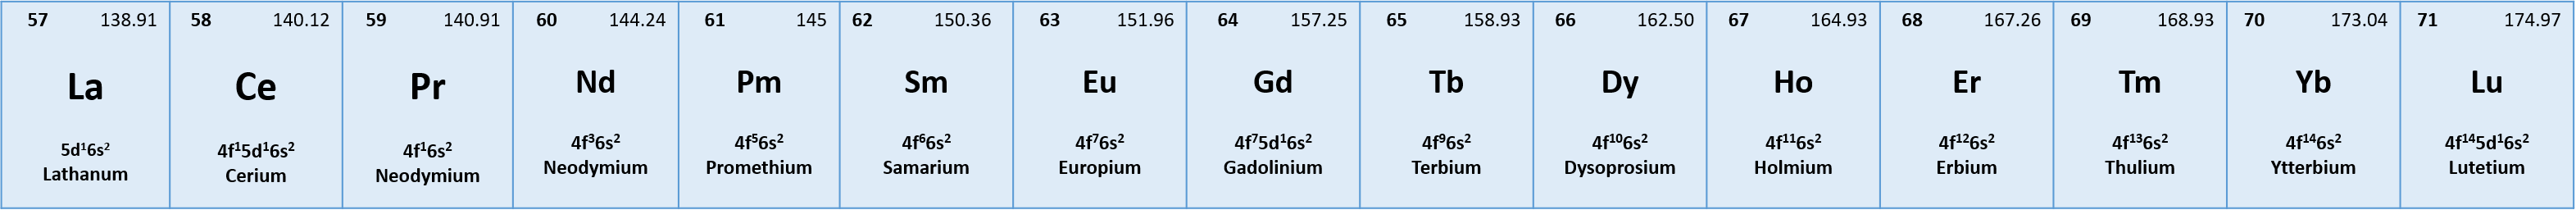
\includegraphics[height=0.08\textwidth,keepaspectratio]{rarearthelements}
\caption{\label{fig:YSOstructure}Lanthanide group elements with electron configuration beginning with [Xe].}
\end{figure}


Rare-earth ions may have an partially filled 4f$^{m}$ ($1 < m < 13$) electron shell, whilst the outer $n = 5$ and $n = 6$ shells are filled. Therefore the paramagnetic center experiences a shielding effect from the environment by the distribution of electrons of the $n = 5$ and $n = 6$ shells. The electronic energy levels of an RE ion can be solved using the central field approximation where each electron moves independently but experiences a nuclear field and an spherically averaged central field due the interaction with other electrons \citep{liu2006spectroscopic}. For a $N$-electron RE ion is given as:

\begin{equation}
\label{eq:freeionHamiltonian}
\hat{H}_{N-el} = \hat{H}_{0} + \hat{H}_{el-el} + \hat{H}_{spin-orbit},
\end{equation} 

\noindent where the dominant $\hat{H}_{0}$ describes the kinetic and potential energy of the electrons in the nuclear field, where $r_{i}$ is the radial distance of electron $i$: 

\begin{equation}
\label{eq:H0}
\hat{H}_{0} = -\sum{N}{i=1} \frac{\hbar^{2}}{2m} \nabla_{i}^{2} - \sum{N}{i=1}\frac{Ze^{2}}/r_{i}. 
\end{equation} 

\noindent The electron-electron Coulomb repulsion is captured by $\hat{H}_{el-el}$:

\begin{equation}
\label{eq:coloumbrep}
\hat{H}_{el-el} = \sum{N}{i<j} \frac{e^{2}}{r_{ij}},
\end{equation}

\noindent where $r_{ij}$ is the distance between pairs of electrons. The fine structure splitting arises due to the interaction of $\mu_{e}$ with the orbital field: 


\begin{equation}
\label{eq:spinorbit}
\hat{H}_{spin-orbit} = \sum{N}{i} \xi(r_{i})\hat{\bm{L}} \cdot \hat{\bm{S}},
\end{equation}

\noindent where $\hat{\bm{L}}$ is the orbital angular momentum operator and $\xi(r_{i})$ is the spin-orbital coupling constant which is a function of $\xi(r_{i})$. This lifts the degeneracy of $^{(2s+1)}L_{j}$ multiplets where the total angular momentum $\bm{j} = \bm{s} + \bm{l}$. 

\begin{table}[h]
 \begin{center}
  \caption{Energy level scales of RE ions}
  \label{tab:REionenergyscale}
  \begin{tabular}{l | c}
  \hline
  Interaction Mechanism & Energy (cm$^{-1}$)\\
  \hline
  Coulomb repulsion & 10$^{4}$\\
  Spin orbit coupling & 10$^{3}$\\
  Crystal field interaction & 10$^{2}$\\
  Hyperfine splitting & 10$^{-3}$-10$^{-1}$\\
  
  \hline
    \end{tabular}
  \end{center}
\end{table}

When ions are placed in a crystal expectation the crystal field produces the dominant Hamiltonian term. However, due to the shielding of the 4f shell the unpaired electrons remain localised to the nucleus and only interact weakly with the ligands~\citep{MALKIN1987131}. The scale of crystal field splitting compared to other energy splitting of other interaction terms is given in Table~\ref{tab:REionenergyscale}. Therefore the crystal field interaction is treated as a perturbation which produces a Stark shift of the multiplets. Additionally the crystal field distorts the electronic orbitals resulting in the highly magnetic anisotropy of RE doped YSO~\citep{abragam2012electron,KOLMAKOVA1996245}. Further splitting of the fine structure occurs due to the electron Zeeman, hyperfine and nuclear Zeeman interaction detailed in Section ~\ref{sec:zeeman} and ~\ref{sec:hyperfine}. The additional, Zero-field interaction and nuclear quadrupole interaction, spin Hamiltonian terms must be included when $S >\frac{1}{2}$ and $I > \frac{1}{2}$, respectively.      

\subsection{\label{sec:YSOdopedYbions}YSO doped with Yb$^{3+}$ ions}
The stable oxidation $+2$ state of Yb is shown in Fig.~\ref{fig:YSOstructure}. However, Yb$^{3+}$ ions have attractive properties due to their 4f$^{13}$ configuration. Yb$^{3+}$ is a paramagnetic rare earth comprising of two energy levels, the ground $^{2}$F$_{5/2}$ and excited $^{2}$F$_{7/2}$ state \citep{PhysRevB.94.155116}. Additionally, the $I \neq 0$ naturally occurring isotopes are $^{171}$Yb$^{3+}$ ($I=\frac{1}{2}$) and $^{173}$Yb$^{3+}$ ($I=\frac{5}{2}$). Therefore, $^{171}$Yb$^{3+}$ doped in YSO provides the simplest RE hyperfine energy structure which can be investigated using pulsed EPR techniques.  

Yb$^{3+}$ ions with a radii of 0.858 $\AA$ substitute Y$^{3+}$ ions in site I and site II approximately equally. The $\bm{g}$ and $\bm{A}$ tensors for Yb$^{3+}$:YSO have be experimentally extracted in Ref.~\citep{PhysRevB.94.155116}. The site I and site II ground $^{2}$F$_{7/2}$ state dimensionless g-tensors are given below as:

 
\begin{equation}
\label{eq:gtensorsiteI}
\bm{g}_{siteI}=\begin{bmatrix}
3.19 & -0.91 & 0.31 \\ 
-0.19 & -0.54 & 0.15\\ 
0.31 & 0.15 & 1.00 \\
\end{bmatrix}_{(D1,D2,b)},
\end{equation}  
  


\begin{equation}
\label{eq:gtensorsite}
\bm{g}_{siteII}=\begin{bmatrix}
-0.32 & -0.86 & -1.21 \\ 
-0.86 & -0.05 & 1.10 \\ 
-1.21 & 1.10 & -2.57 \\
\end{bmatrix}_{(D1,D2,b)}.
\end{equation}  


Additionally the ground state anisotropic $\bm{A}$ tensors (in MHz) for site I and site II are given below as:


\begin{equation}
\label{eq:AtensorsiteI}
\bm{A}_{siteI}=\begin{bmatrix}
-3844 & 1356 & 1909 \\ 
1356 & -2257 & 162 \\ 
1909 & 162 & -1340 \\
\end{bmatrix}_{(D1,D2,b)},
\end{equation}  

\begin{equation}
\label{eq:AtensorsiteII}
\bm{A}_{siteI}=\begin{bmatrix}
1054 & -503 & -894 \\ 
-503 & 232 & 660\\ 
-894 & 660 & -4554 \\
\end{bmatrix}_{(D1,D2,b)}.
\end{equation}  

The spin relaxation time $T_{1}$ of unpaired electrons spins of Yb$^{3+}$ is highly temperature dependent. This is due to spin coupling to vibrations of the host lattice. For very low temperature (<4 K) the direct process dominates. The rate of the direct process for the case where $k_{B}T$ is greater than the Zeeman splitting is:

\begin{equation}
\label{eq:coloumbrep}
R_{dp} \approx \frac{2\alpha_{D}(\theta)k_{B} T g^{2}_{eff} B^{4}}{\mu},
\end{equation}

\noindent where the constant $\alpha_{D}(\theta)$ varies with crystal orientation as determined in Ref.~\citep{PhysRevB.97.064409}. This process results in direct phonon absorption from the lattice or phonon emission. 


\begin{figure}[h]
\centering
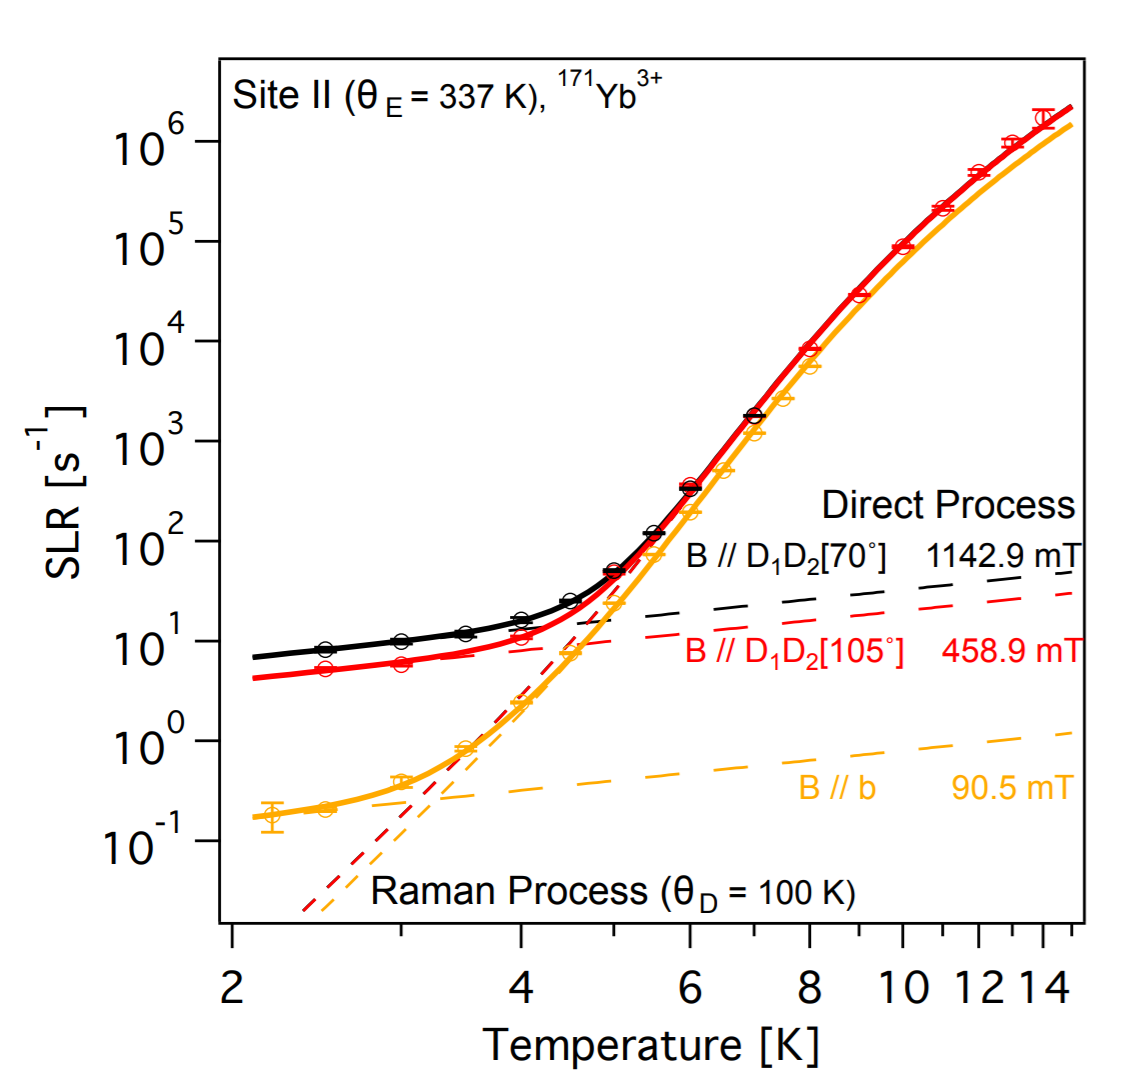
\includegraphics[height=0.4\textwidth,keepaspectratio]{spinrelaxationtime}
\caption{\label{fig:spinrelaxation}Spin relaxation of $^{171}$Yb$^{3+}$:YSO measurements for Site II. Each colour represents a different orientation of crystal with respect to an applied magnetic field. The solid lines are the fit based on a model including both the direct and two-phonon processes. The large dashed line illustrate is the single phonon fit model and the smaller dashed line represents the two-phonon process fit model \citep{PhysRevB.97.064409}.}
\end{figure}

As temperature increases two phonon process become dominant. The Raman process occurs where there is a virtual transition of the spin state to an intermediate state due to the absorption of a phonon. This is followed by emission of phonon with a higher energy due to the transition to the lower spin state. The spin relaxation times has a dependence on temperature which can vary between $T^{-5}-T^{-9}$.Additionally the Orbach process describes the resonant excitation of phonons to a highly excited states which has a temperature dependence of $exp{-\Delta/k_{B}T}$ where $\Delta$ is the excitation energy \citep{weil1994electron,doi:10.1002/pssb.2221170202}.

   




    \section{\label{sec:strain}Strain}
The aim of this research project is the investigate the effect of strain on the A and g-tensors due to changing the distribution of electron and nuclear spins in $^{171}$Yb doped YSO. Mechanical strain is induced by applying stress to along a crystal axis similarly as for the Si:P sample in Ref.~\citep{PhysRevLett.120.167701}. This experiment aims to provide insight into the strain induced as a result of spin doped substrates with a patterned superconducting resonator on the surface being cooled to cryogenic temperatures. The compression of the materials used in fabrication as a function of temperature is expected to induce strain at the interface of substrates and perturb the bulk properties of the crystal. Relevant coefficients of thermal expansion for spin substrates and commonly used materials are presented in Table~\ref{tab:thermalexpansions} which has been advised by Ref.~\citep{mansirthesis}. 

\begin{table}[h]
 \begin{center}
  \caption{Thermal expansion coefficients for material used for nanofabricated devices~\citep{Sato:14,doi:10.1063/1.323747,PhysRev.60.597,1674-1056-21-12-127103}.}
  \label{tab:thermalexpansions}
  \begin{tabular}{l | c}
  \hline
  Material & Thermal expansion coefficient \\
  & at 300 K ($\times 10^{-6}$ K$^{-1}$) \\
  \hline
   Y$_{2}$SiO$_{5}$ & 6.3\\
  Silicon & 2.6\\
  Aluminum & 22.5\\
  Aluminium oxide & 8.1\\
  Niobium Nitride & 4.2\\
  \hline
    \end{tabular}
  \end{center}
\end{table}

Therefore, understanding of relationship between stress and strain for this substrate is guided by referring to Ref.~\citep{doi:10.1002/crat.2170211204} and Ref.~\citep{wooster1973tensors}. In this section the compliance matrix which relates stress to strain is obtained in the conventional ($D1,D2,b$) co-ordinate frame.    

\subsection{Stress and Strain Tensors}
\label{sec:stressandstrain}
Following Hooke's law, provided the stress applied to a solid object is below the elastic limit, the deformation of the object is reversible when no longer acted on by stress. In three-dimensions the variation of displacement $u_{i}$ with position $x_{i}$ in the object results is

\begin{equation}
\label{eq:generalmatrixnotation}
e_{ij}=\frac{\partial u_{i}}{\partial x_{i}}, \;\;\;\; (i,j = 1,2,3).
\end{equation} 

\noindent The object undergoing rotation around a chosen axis $u_{i}$ with no strain sets the condition that any displacement perpendicular to the axis is $u_{i}x_{i}=0$ and thus requires that $e_{ij}$ is antisymmetric. The stiffness tensor $[S]$ is a 4th-rank tensor which relates the 2nd-rank stress $[\sigma]$ and strain $[\epsilon]$ tensors, in the component form as $\sigma_{ij}=c_{ijkl}\epsilon_{kl}$ where $ijkl=1,2,3$. This results from the inability to describe normal and shear stress/strain components by a single vector. 

The elements of tensors, $[\sigma]$ and $[\epsilon]$ given in Eq.~\ref{eq:stresstensor} and Eq.~\ref{eq:straintensor}, along the matrix diagonal are acting normal to the crystal surface and the off-diagonal elements give the shear components:     

\begin{equation}
\label{eq:stresstensor}
[\sigma]=\begin{bmatrix}
\sigma_{11} & \sigma_{21} & \sigma_{31} \\ 
\sigma_{12} & \sigma_{22}  & \sigma_{32}\\ 
\sigma_{13} & \sigma_{23} & \sigma_{33}
\end{bmatrix},
\end{equation} 

\begin{equation}
\label{eq:straintensor}
[\epsilon]=\begin{bmatrix}
\epsilon_{11} & \epsilon_{21} & \epsilon_{31} \\ 
\epsilon_{12} & \epsilon_{22}  & \epsilon_{32}\\ 
\epsilon_{13} & \epsilon_{23} & \epsilon_{33}.
\end{bmatrix}.
\end{equation} 


\noindent There are initially 81 independent stiffness elements of $c_{ijkl}$. However, by definition $\epsilon$ is the symmetric part of $e_{ij}$. Therefore, the stress tensor simplifies such that if $i\neq j$ then $\epsilon_{ij} = \epsilon_{ji}$. Similarly the stress tensor is also symmetric. Thus considering cases where only normal or a pair of shear components are the nonzero elements of the tensor, this results in the conditions that $c_{ijkl}=c_{jilk}$ and $c_{ijkl}=c_{jilk}$. 

Consequently the number of independent components of $c_{ijkl}$ reduces to 36. Additionally the compliance tensor $s$ in component form is given as $\epsilon_{ij}=s_{ijkl}\sigma_{kl}$ and is simplified to 36 independent components. Similarly the compliance tensor $[S]$, which relates $[\epsilon]$ to $[\sigma]$ as $\epsilon_{ij}=s_{ijkl}\sigma_{kl}$, index symmetry is $s_{ijkl}=s_{jilk}$ and $s_{ijkl}=s_{jilk}$. Due to the symmetry of $[C]$ (and $[S]$) the stress and strain components can be converted into the matrix (or Voigt) notation and then into vector notation such that:

\begin{equation}
\label{eq:stresstensorsimiplified}
\begin{bmatrix}
\sigma_{11} & \sigma_{12} & \sigma_{13} \\ 
\sigma_{12} & \sigma_{22}  & \sigma_{23}\\ 
\sigma_{13} & \sigma_{23} & \sigma_{33}
\end{bmatrix}\leftrightarrow 
\begin{bmatrix}
\sigma_{1} & \sigma_{6} & \sigma_{5} \\ 
\sigma_{6} & \sigma_{2}  & \sigma_{4}\\ 
\sigma_{5} & \sigma_{4} & \sigma_{3}
\end{bmatrix} \leftrightarrow 
\begin{bmatrix}
\sigma_{1}\\ 
\sigma_{2}\\ 
\sigma_{3}\\ 
\sigma_{4}\\ 
\sigma_{5}\\ 
\sigma_{6}
\end{bmatrix},
\end{equation} 

\begin{equation}
\label{eq:straintensorsimplified}
\begin{bmatrix}
\epsilon_{11} & \epsilon_{12} & \epsilon_{13} \\ 
\epsilon_{12} & \epsilon_{22}  & \epsilon_{23}\\ 
\epsilon_{13} & \epsilon_{23} & \epsilon_{33}
\end{bmatrix} \leftrightarrow 
\begin{bmatrix}
\epsilon_{1} & \frac{1}{2}\epsilon_{6} & \frac{1}{2}\epsilon_{5} \\ 
\frac{1}{2}\epsilon_{6} & \epsilon_{2}  & \frac{1}{2}\epsilon_{4}\\ 
\frac{1}{2}\epsilon_{5} & \frac{1}{2}\epsilon_{4} & \epsilon_{3}
\end{bmatrix} \leftrightarrow 
\begin{bmatrix}
\epsilon_{1}\\ 
\epsilon_{2}\\ 
\epsilon_{3}\\ 
\epsilon_{4}\\ 
\epsilon_{5}\\ 
\epsilon_{6}
\end{bmatrix},
\end{equation}

\noindent where for clarity $\bm{\sigma}$ and $\bm{\epsilon}$ will refer to vector notation such that ie. $\bm{\epsilon}=\begin{bmatrix} \epsilon_{1} & \epsilon_{2} & \epsilon_{3} & \epsilon_{4} & \epsilon_{5} & \epsilon_{6} \\ \end{bmatrix}^{T}$.


It is clear the factors of $\frac{1}{2}$ in Eq.~\ref{eq:straintensorsimplified} arise selecting $\epsilon_{ij}$ for certain values of $i,j$ and writing out $\epsilon_{ij}=s_{ijkl}\sigma_{kl}$ for $k,l=1,2,3$ then transforming to the matrix notation and using the symmetry of the $s_{ijkl}$ subscripts. Therefore, the general form in the matrix notation is given as: 

\begin{equation}
\label{eq:generalmatrixnotation}
\sigma_{i} = c_{ij}\epsilon_{j} \;\;\;\; (i,j = 1,2...,6),
\end{equation} 

\noindent where the 6$\times$6 stiffness matrix, $[c]$ and the 6$\times$6 compliance matrix, $[s]$ are related as $[s]=[c]^{-1}$. 

The number of independent matrix elements further reduces to 21 as $[c]$ is determined to be symmetric. Derivation of this property is obtained by equating the change in the work done $dW=\sigma_{i}d\epsilon_{i}$, by applying a stress to produce a reversible and isotropic strain on the face of a cubic crystal, to the increase Helmholtz free energy in matrix notation as:

\begin{equation}
\label{eq:freeenergyequate}
d\psi =c_{ij}\sigma_{j}d\epsilon_{i},
\end{equation} 


\noindent then differentiating each side of Eq.~\ref{eq:freeenergyequate} by $\epsilon_{j}$ where the order of differentiating $\Psi$ is unimportant. This results in the symmetry $c_{ij}=c_{ji}$ and reciprocal matrix is also symmetric such that $s_{ij}=s_{ji}$.  

\subsection{Monoclinic stiffness matrix}

The number of independent nonzero elements of $c_{ij}$ further reduces depending on the symmetry of the crystal. Since YSO is anisotropic and monoclinic the number of nonzero independent elements of $[c]$ is 13. This is determined as the energy density function: 

\begin{equation}
\label{eq:energyW}
W=\frac{1}{2}c_{ij}\epsilon_{i}\epsilon_{j},
\end{equation}

\noindent must be invariant under coordinate transformation where $c_{ij}=c_{ji}$. Therefore, If we consider the crystal in the ($D1,b,D2$) frame, then $D1-D2$ is the plane around the symmetry b-axis. The change of axis is given as: 

\begin{equation}
\label{eq:planofsymmetry}
D1'=D1, \;\;\;\; b' = -b, \;\;\;\; \textrm{and} \;\;\;\; D2'=D2.
\end{equation}

One way to transform between reference frame in the full tensor notation is given as $\epsilon_{ij}=a_{ki}a_{lj}\epsilon_{ij}$ where for ie. $a_{ij}$, which is the partial differentiation of crystal axis $i$ with respect to crystal axis $j$. Thus: 

\begin{equation}
\label{eq:apartialdiff}
a_{ij}=\frac{\partial i}{\partial j}=\delta_{ij}, 
\end{equation}

\noindent where $\frac{\partial i}{\partial j}=-\delta_{ij}$ if $i,j=b$ and $i\neq j$, and $\frac{\partial i}{\partial j}=\delta_{ij}$ if $i,j=D1,D2$. Additionally, for $\epsilon_{4},\epsilon_{5}$ and $\epsilon_{6}$ conversion back to $\epsilon_{ij}$ notation is given by Eq.~\ref{eq:straintensorsimplified}. Therefore, the $[c]$ matrix for the crystal symmetry is: 


\begin{equation}
\label{eq:13elementC}
[c]=\begin{bmatrix}
c_{11} & c_{12} & c_{13} & 0 & c_{15} & 0 \\
& c_{22} & c_{23} & 0 & c_{25} & 0 \\
& & c_{33} & 0 & c_{35} & 0 \\
& Sym. & & c_{44} & 0 & c_{46} \\
& & & & c_{55} & 0 \\
& & & & & c_{66} \\
\end{bmatrix} 
\end{equation}

where there are 13 nonzero independent elements. 

% space group?

\subsection{\label{sec: YSO stiffness matrix}{YSO stiffness matrix}}

%The lattice structural parameters such as the crystallographic axis, $a$,$b$ and $c$, of the unit cell, in an appropriate space group, are determined based on density functional theory with localised density approximation and ultrasoft pseudopotentials. Homogeneous strain is applied and optimisation of the atomic positioning for the established unit cell allows linear fitting of the stress resulting from the strain. Therefore the stiffness matrix can be determined. The stiffness matrix elements are referred to as second-order elastic coefficients since they provide the second derivative of the total energy with respect to atomic displacements~\citep{0953-8984-13-2-302,doi:10.1111/jace.12764}. %The lattice structural parameters such as the crystallographic axis, $a$,$b$ and $c$, of the unit cell, in an appropriate space group, are determined based on density functional theory with localised density approximation and ultrasoft pseudopotentials~\citep{0953-8984-13-2-302}. 

Bravais lattices are made up indefinite unit cells defined by the lattice vectors of length, $a$, $b$ and $c$ and related through arbitrary angles, $\alpha$, $\beta$ and $\gamma$. There are 230 space groups which result from the combination of Bravais lattices and symmetry operations. Comparison of the $C2/c$ with the $I2/a$ space group is shown in Fig~\ref{fig:crystalspacegroups} where the lattice parameters for $I2/a$ is given in Table.~\ref{tab:I2alatticeparam}. The lattice structural parameters such as the crystallographic axis, $a$,$b$ and $c$, of the unit cell, in an appropriate space group, are determined based on density functional theory with localised density approximation and ultrasoft pseudopotentials~\citep{0953-8984-13-2-302}. Homogeneous strain is applied and optimisation of the atomic positioning, for the established unit cell, allows linear fitting of the stress resulting from the strain enables the stiffness matrix to be determined. The stiffness matrix elements are referred to as second-order elastic coefficients since they provide the second derivative of the total energy with respect to atomic displacements~\citep{doi:10.1111/jace.12764}. Theoretical second-order elastic coefficients are given in Table~\ref{tab:elasticcoefficients} in GPa for the corresponding Y$_{2}$SiO$_{5}$ unit cell in the $B2/b$~\citep{doi:10.1111/jace.12764} and $C2/c$~\citep{Ceramics} space group for comparison. 

The most conventional space group to describe the unit cell of a monoclinic crystal is the $C2/c$ which is $C$-face centered lattice~\citep{conventionalcells}. Therefore, the $C2/c$ elastic coefficients are presented in Eq.~\ref{eq:stiffnessmatrixC} with the corresponding lattice parameters compared to experimentally determined values in Table~\ref{tab:latticeparam}.Due to the ambiguity of the calculated [$c$] reference frame, documentation for the tool ElaStic\citep{ElaStic} which can be used to compute second-order elastic coefficients was consulted. This revealed for a monoclinic crystal with $b$ as the unique axis the Cartesian coordinate frame is $\textbf{a}=(a,0,0)$, $\textbf{b}=(0,b,0)$ and $\textbf{c}=(c \cos{\beta},0,c \sin{\beta})$. 

\begin{table}[h]
 \begin{center}
  \caption{Y$_{2}$SiO$_{5}$ $C2/c$ lattice parameters}
  \label{tab:latticeparam}
  \begin{tabular}{l | c c}
  \hline
  Lattice constants & Experimental~\citep{Cong:ko5080} & Theoretical~\citep{Ceramics} \\
  \hline
  a ($\AA$) & 14.37 & 14.25 \\
  b ($\AA$) & 6.71 & 6.59 \\
  c ($\AA$) & 10.39 & 10.23 \\
  $\beta$ ($\deg$) & 122.2 & 122.3 \\
  \hline
    \end{tabular}
  \end{center}
\end{table}




The stiffness matrix in the $C2/c$ space group and $(\textbf{a},\textbf{b},\textbf{c})$ is


\begin{equation}
\label{eq:stiffnessmatrixC}
[c]=
\begin{bmatrix}
226 & 59 & 88 & 0 & 5 & 0 \\
& 156 & 27 & 0 & -0.3 & 0 \\
& & 201 & 0 & -0.2 & 0 \\
& Sym. & & 44 & 0 & 10 \\
& & & & 63 & 0 \\
& & & & & 67 \\
\end{bmatrix}_{(\textbf{a},\textbf{b},\textbf{c})}.
\end{equation}

However since the sample is cut along the optical axis and uniaxial stress will be applied along each of those axis, $[c]$ must be transformed accordingly. The orientation of the $(D1,b,D2)$ reference frame with respect to the $C2/c$ crystallographic axes is given in Fig.~\ref{fig:D1bD2abc} where lattice parameter $b$ is parallel with respect to the optical axis $b$. Thus $\theta=$23.8 $\deg$ anticlockwise rotation around the y-axis is required to rotate the coordinate frame from $(\textbf{a},\textbf{b},\textbf{c})$ to $(D1,b,D2)$. Therefore the rotation matrix $R_{m}$ is:

\begin{equation}
\label{eq:rotateatoD1}
\begin{bmatrix}
r_{11} & r_{12} & r_{13} \\
r_{21} & r_{22} & r_{23} \\
r_{31} & r_{32} & r_{33} \\
\end{bmatrix}=
\begin{bmatrix}
\cos{(\beta')} & 0 & \sin{(\beta')} \\
0 & 1 & 0 \\
-\sin{(\beta')} & 0 & cos{(\beta')}
\end{bmatrix}
\end{equation}

\noindent where $\beta'=360 \deg - \beta$. 


Then the second-rank tensor transformation between $[\epsilon]$ in the $(\textbf{a},\textbf{b},\textbf{c})$ frame and $[\epsilon^{'}]$ in the (D1,b,D2) frame can be obtain following Eq.~\ref{eq:epsilontransformation} 

\begin{equation}
\label{eq:epsilontransformation}
\epsilon_{ij}^{'}=r_{ik}r_{jl}\epsilon_{kl},
\end{equation}

where for example $\epsilon_{11} = r_{11}^{2}\epsilon_{11} + r_{12}^{2}\epsilon_{22} + r_{13}^{2}\epsilon_{13} +2r_{12}r_{13}\epsilon_{23} + 2r_{11}r_{13}\epsilon_{13} + 2r_{11}r_{12}\epsilon_{12}$. Then similarly as in Eq.~\ref{eq:straintensorsimplified} in matrix notation this becomes $\epsilon_{1}=r_{11}^{2}\epsilon_{1} + r_{12}^{2}\epsilon_{2} + r_{13}^{2}\epsilon_{3} + r_{12}r_{13}\epsilon_{4} + r_{11}r_{13}\epsilon_{5} + r_{11}r_{12}\epsilon_{6}$. The transformation to matrix notation for ie. $\epsilon_{12}=\frac{1}{2}\epsilon_{6}$ must not be neglected. Since it can be shown that $[\sigma]=[T_{\epsilon}][\sigma^{'}]$, the transformation tensor $[T_{\epsilon}]$ in the matrix notation is: 

\begin{equation}
\label{eq:transformationmatrix}
\begin{bmatrix}
r_{11}^{2} & r_{12}^{2} & r_{13}^{2} & r_{12}r_{13} & r_{11}r_{13} & r_{11}r_{12} \\
r_{21}^{2} & r_{22}^{2} & r_{23}^{2} & r_{21}r_{23} & r_{21}r_{23} & r_{21}r_{22} \\
r_{31}^{2} & r_{32}^{2} & r_{33}^{2} & r_{32}r_{33} & r_{31}r_{33} & r_{31}r_{32} \\
2r_{21}r_{31} & 2r_{22}r_{32} & 2r_{23}r_{33} & (r_{22}r_{33}+r_{23}r_{32}) & (r_{21}r_{33}+r_{23}r_{31}) & (r_{21}r_{32}+r_{22}r_{31}) \\
2r_{11}r_{31} & 2r_{12}r_{32} & 2r_{13}r_{33} & (r_{12}r_{33}+r_{13}r_{32}) & (r_{11}r_{33}+r_{13}r_{31}) & (r_{11}r_{32}+r_{12}r_{31}) \\
2r_{11}r_{21} & 2r_{12}r_{22} & 2r_{12}r_{23} & (r_{12}r_{23}+r_{13}r_{22}) & (r_{13}r_{22}+r_{13}r_{21}) & (r_{11}r_{22}+r_{12}r_{21}) \\
\end{bmatrix}.
\end{equation}


To check Eq.~\ref{eq:stiffnessmatrixD1bD2} produces sensible results a simple $R_{y}(\pi/2)$ rotation was tested initially.

\begin{equation}
\label{eq:stiffnessmatrixD1bD2}
[c]_{(D1,b,D2)}=[T_{\epsilon}][c]_{(\textbf{a},\textbf{b},\textbf{c})}[T_{\epsilon}]^{T}.
\end{equation}

$[c]_{(D1,b,D2)}$ is then computed as: 

\begin{equation}
\label{eq:stiffnessmatrixC}
[c]_{(D1,b,D2)}=\begin{bmatrix}
171 & 36 & 113 & 0 & 22.5 & 0 \\
& 156 & 43.5 & 0 & -28.8 & 0 \\
& & 139.3 & 0 & -33.1 & 0 \\
& Sym. & & 51.4 & 0 & -14.7 \\
& & & & 220.4 & 0 \\
& & & & & 59.6 \\
\end{bmatrix}_{(D1,b,D2)}.
\end{equation}

\noindent Furthermore, since $[g]$ and $[A]$ are conventionally presented in the $(D1,D2,b)$ coordinate frame~\citep{PhysRevB.94.155116}, it is advantageous for Eq.\ref{eq:stiffnessmatrixC} to be transformed to this frame. In this case $R_{m}$ is:

\begin{equation}
\label{eq:rotateatoswitchbD2axis}
\begin{bmatrix}
r_{11} & r_{12} & r_{13} \\
r_{21} & r_{22} & r_{23} \\
r_{31} & r_{32} & r_{33} \\
\end{bmatrix}=
\begin{bmatrix}
1 & 0 & 0 \\
0 & 0 & 1 \\
0 & 1 & 0 \\
\end{bmatrix},
\end{equation}

\noindent which allows conversion of $(D1,b,D1)\leftrightarrow (D1,D2,b)$. Similarly, using Eq.~\ref{eq:transformationmatrix} and Eq.~\ref{eq:stiffnessmatrixD1bD2}, $[c]_{(D1,b,D2}$ is transformed to:

\begin{equation}
\label{eq:stiffnessmatrixCD1D2b}
[c]_{(D1,D2,b)}=\begin{bmatrix}
171 & 113 & 36 & 0 & 0 & 22.5 \\
& 139.3 & 43.5 & 0 & 0 & -33.1 \\
& & 156 & 0 & 0 & 28.8 \\
& Sym. & & 51.4 & -14.7 & 0 \\
& & & & 59.6 & 0 \\
& & & & & 220.4 \\
\end{bmatrix}_{(D1,D2,b)}.
\end{equation}.

\noindent Finally in this experiment a unaxial linear stress ($\epsilon_{1}, \epsilon_{2}$ or $\epsilon_{3}$) is applied to the crystal, thus $[s]_{(D1,D2,b)}$ must be to calculated to determine $\bm{\epsilon}_{D1,D2,b}$. Therefore matrix inversion of $[c]$ provides:

\begin{equation}
\label{eq:stiffnessmatrixCD1D2b}
[s]_{(D1,D2,b)}=\begin{bmatrix}
14.8 & -12.6 & -0.5 & 0 & 0 & -3.5 \\
& 18.9 & -1.6 & 0 & 0 & 3.9 \\
& & 7.1 & 0 & 0 & 0.7 \\
& Sym. & & 20.9 & 5.2 & 0 \\
& & & & 18.0 & 0 \\
& & & & & 5.6 \\
\end{bmatrix}_{({D1},{D2},{b})}.
\end{equation}.

in units of pPa$^{-1}$. Now using Eq.~ref{eq:stiffnessmatrixCD1D2b} the induced $\bm{\epsilon}_{(D1,D2,b)}$ can be computed stress applied to each dielectric axis. The result for each case is always three nonzero linear terms and a nonzero shear term.   


\section{Spin-Strain Interaction}
Now that the relationship between strain and stress can be successfully calculated, the ability to relate the strain to the spin Hamiltonian components is considered. Since $[A]$ and $[g]$ are additionally second-order symmetric tensors and based on the conditions discussed in Sec.~\ref{sec:stressandstrain} it can be determined that matrices, $[\mathcal{G}]$ and $[\mathcal{A}]$, relating $[\sigma]$ to $[g]$ and $[A]$ will also be symmetric. Further reduction beyond 21 independent matrix elements is not possible due to trivial $C1$ symmetry of the Y$^{+3}$ ion sites. Eq.~\ref{eq:gtosigma} and Eq.~\ref{eq:Atosigma} relate vectors $\bm{g}$ and $\bm{A}$ to $\bm{\epsilon}$:



\begin{equation}
\label{eq:gtosigma}
g=\begin{bmatrix}
g_{1} \\
g_{2} \\
g_{3} \\
g_{4} \\
g_{5} \\
g_{6} \\
\end{bmatrix}=
\begin{bmatrix}
\mathcal{G}_{11} & \mathcal{G}_{12} & \mathcal{G}_{13} & \mathcal{G}_{14}
& \mathcal{G}_{15} & \mathcal{G}_{16} \\
& \mathcal{G}_{22} & \mathcal{G}_{23} & \mathcal{G}_{24} & \mathcal{G}_{25} & \mathcal{G}_{26} \\
& & \mathcal{G}_{33} & \mathcal{G}_{34} & \mathcal{G}_{35} & \mathcal{G}_{36} \\
& Sym. & & \mathcal{G}_{44} & \mathcal{G}_{45} & \mathcal{G}_{46} \\
& & & & \mathcal{G}_{55} & \mathcal{G}_{56} \\
& & & & & \mathcal{G}_{66} \\
\end{bmatrix}_{(D1,D2,b)}
\begin{bmatrix}
\epsilon_{1} \\
\epsilon_{2} \\
\epsilon_{3} \\
\epsilon_{4} \\
\epsilon_{5} \\
\epsilon_{6} \\
\end{bmatrix},
\end{equation}  

  
\begin{equation}
\label{eq:Atosigma}
A=\begin{bmatrix}
A_{1} \\
A_{2} \\
A_{3} \\
A_{4} \\
A_{5} \\
A_{6} \\
\end{bmatrix}=
\begin{bmatrix}
\mathcal{A}_{11} & \mathcal{A}_{12} & \mathcal{A}_{13} & \mathcal{A}_{14}
& \mathcal{A}_{15} & \mathcal{A}_{16} \\
& \mathcal{A}_{22} & \mathcal{A}_{23} & \mathcal{A}_{24} & \mathcal{A}_{25} & \mathcal{A}_{26} \\
& & \mathcal{A}_{33} & \mathcal{A}_{34} & \mathcal{A}_{35} & \mathcal{A}_{36} \\
& Sym. & & \mathcal{A}_{44} & \mathcal{A}_{45} & \mathcal{A}_{46} \\
& & & & \mathcal{A}_{55} & \mathcal{A}_{56} \\
& & & & & \mathcal{A}_{66} \\
\end{bmatrix}_{(D1,D2,b)}
\begin{bmatrix}
\epsilon_{1} \\
\epsilon_{2} \\
\epsilon_{3} \\
\epsilon_{4} \\
\epsilon_{5} \\
\epsilon_{6} \\
\end{bmatrix}.
\end{equation} 

Similarly as in Eq.~\ref{eq:straintensorsimplified}, the following transformation of $[g]$ and $[A]$ completed to obtain the vector notation:

\begin{equation}
\label{eq:gsimplified}
\begin{bmatrix}
g_{11} & g_{12} & g_{13} \\ 
g_{12} & g_{22}  & g_{23}\\ 
g_{13} & g_{23} & g_{33}
\end{bmatrix} \leftrightarrow 
\begin{bmatrix}
g_{1} & \frac{1}{2}g_{6} & \frac{1}{2}g_{5} \\ 
\frac{1}{2}g_{6} & g_{2}  & \frac{1}{2}g_{4}\\ 
\frac{1}{2}g_{5} & \frac{1}{2}g_{4} & g_{3} \\
\end{bmatrix} \leftrightarrow 
\begin{bmatrix}
g_{1}\\ 
g_{2}\\ 
g_{3}\\ 
g_{4}\\ 
g_{5}\\ 
g_{6}
\end{bmatrix},
\end{equation}

and

\begin{equation}
\label{eq:Asimplified}
\begin{bmatrix}
A_{11} & A_{12} & A_{13} \\ 
A_{12} & A_{22}  & A_{23}\\ 
A_{13} & A_{23} & A_{33}
\end{bmatrix} \leftrightarrow 
\begin{bmatrix}
A_{1} & \frac{1}{2}A_{6} & \frac{1}{2}A_{5} \\ 
\frac{1}{2}A_{6} & A_{2}  & \frac{1}{2}A_{4}\\ 
\frac{1}{2}A_{5} & \frac{1}{2}A_{4} & A_{3} \\
\end{bmatrix}_{(D1,b,D2)} \leftrightarrow 
\begin{bmatrix}
A_{1}\\ 
A_{2}\\ 
A_{3}\\ 
A_{4}\\ 
A_{5}\\ 
A_{6}
\end{bmatrix}.
\end{equation}

Due to low symmetry of YSO and Y$^{+3}$ ions, each element of $\bm{g}$ and $\bm{A}$ provides an expression containing linear and tensile $\bm{\epsilon}$ elements multiplied by unknown $[\mathcal{G}]$ and $[\mathcal{A}]$ coefficients. In order to gain information about the coefficients a select few elements would have to be dominant such that many coefficients could be approximated as zero.



    \chapter{Experimental Methods}
\section{\label{sec:EPRexperimentsetup}EPR Experiment Set-up}
This section discussed the experiment apparatus used to complete the experiments detailed in section. To complete pulsed ESR of a spin system, the main experimental set up requirements include: a cooling system, external magnetic fields, a spectrometer and a resonator. 


Since the spin relaxation rate decreases as a function of temperature, as demonstrated in Fig.~\ref{fig:spinrelaxation}, EPR measurements are completed at $\approx$ 7 K. This temperature is achieved using a liquid helium flow cryostat which reaches the base temperature of 4.2 K. The 20 mm radius sample chamber is surrounded by a outer layer. The outer chamber layer is pumped to 10$^{-5}$ torr to provide thermal insulation. Liquid helium is then pumped from an external dewar via a coxial transfer arm around the chamber before being released to the atmosphere. The cooling of the sample is set by adjusting the liquid helium flow rate and a potential integral derivative (PID) temperature controller, which regulates heating of an element inside the cryostat. The cryostat is secured between the Helmhotz coil configuration of the Bruker electromagnet as shown in Fig. . The magnetic field, $B_{0}$ with a maximum 1 T, is generated between the magnet poles by use of a power supply which applies a current around the large wire coils and is adjusted by a feedback magnetic field controller. The sample should be secured in the centre point between the two coils where the field generated is most homogeneous.       

The Bruker 4118X-MD5W1 probe contains a dielectric ring sapphire crystal resonator capable of hosting samples with a diameter up to 5 mm. The boundary conditions of the electromagnetic wave within the cavity dictates that TE$_{01}$ is the dominant cavity mode. Therefore the magnetic field is parallel to wave propagation direction and thus generates a homogeneous field within the cavity perpendicular to $B_{0}$. High power microwave pulses are sent to the cavity via a coaxial cable transmission. The oscillating $B_{1}$ field is generated by the coupling between the applied pulses and the resonator cavity field. The X-band resonator has a tunable $Q$ factor and centre frequency of $f_{c} \approx 9.7$ GHz. Changing the separation, and thus the coupling, of the coaxial antenna and the resonator enables a small degree of tuning of the cavity $f_{c}$ and $Q$ by introducing a perturbation to the cavity radiation field. The setting of the $Q$ factor for EPR spectroscopy of Yb$^{3+}$:YSO was between $300-400$. The ESR probe is shown in Fig.().        

\begin{figure}[h]
\centering
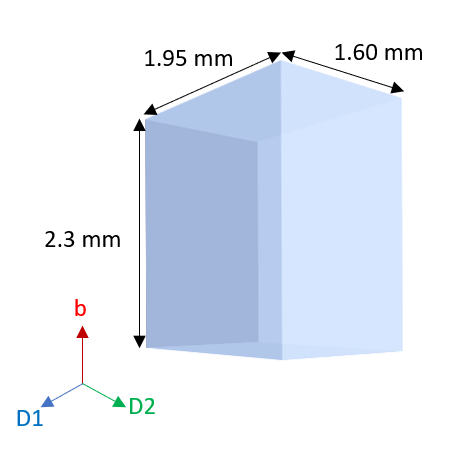
\includegraphics[height=0.4\textwidth,keepaspectratio]{crystaldimesions}
\caption{\label{fig:crystaldimesions} The dimensions of the $^{171}$Yb$^{3+}$:YSO sample used to complete mechanical strain experiments.}
\end{figure}

The magnetisation vector, $\bm{M}$ of excited paramagnetic centres process around $\bm{B_{0}}$ generates a oscillating magnetic field which is detected via the coaxial cable as an AC voltage signal. Typically ESR experiments are completed where the sample are placed into a glass tube holder which is connected to fiberglass rod, where the rod is secured inside the probe such that the sample is in the centre of the resonator. However, in order to investigate the effect of strain on a $^{209}$Bi in isotropically enriched $^{28}$Si in Ref.~\citep{PhysRevLett.120.167701} a costume sample mount was fabricated and connected to the fiberglass rod. The mount was made from a Polyether ether ketone (PEEK) thermoplastic extends into the centre of the cavity. The cylindric hole is drilled into the end of the mount where a fabricated acrylic sample holder secures the isotropic sample. An aluminum base plate which sits on the bottom of cryostat and a second thermoplastic piece extends upwards to meet the mount and also has a milled insert to secure the sample from below. The mount rotates freely and the base remains stationary. 

Due to anisotropy of Yb$^{3+}$ doped in the YSO crystal, the sample mount must be adapted to secure the doped YSO sample which has been cut along the orthogonal dielectric axes. Therefore a separate adapter must be fabricated for each dielectric axis to be orientated perpendicular to $\bm{B_{0}}$ where the crystal dimensions given in Fig.~\ref{fig:crystaldimesions}. Further description of the sample mounting in the cryostat and the sample holder fabrication is presented in the section below.   




\subsection{Fabrication}
\begin{figure}[H]
    \centering
    \begin{subfigure}[b]{0.35\textwidth}
        \centering
 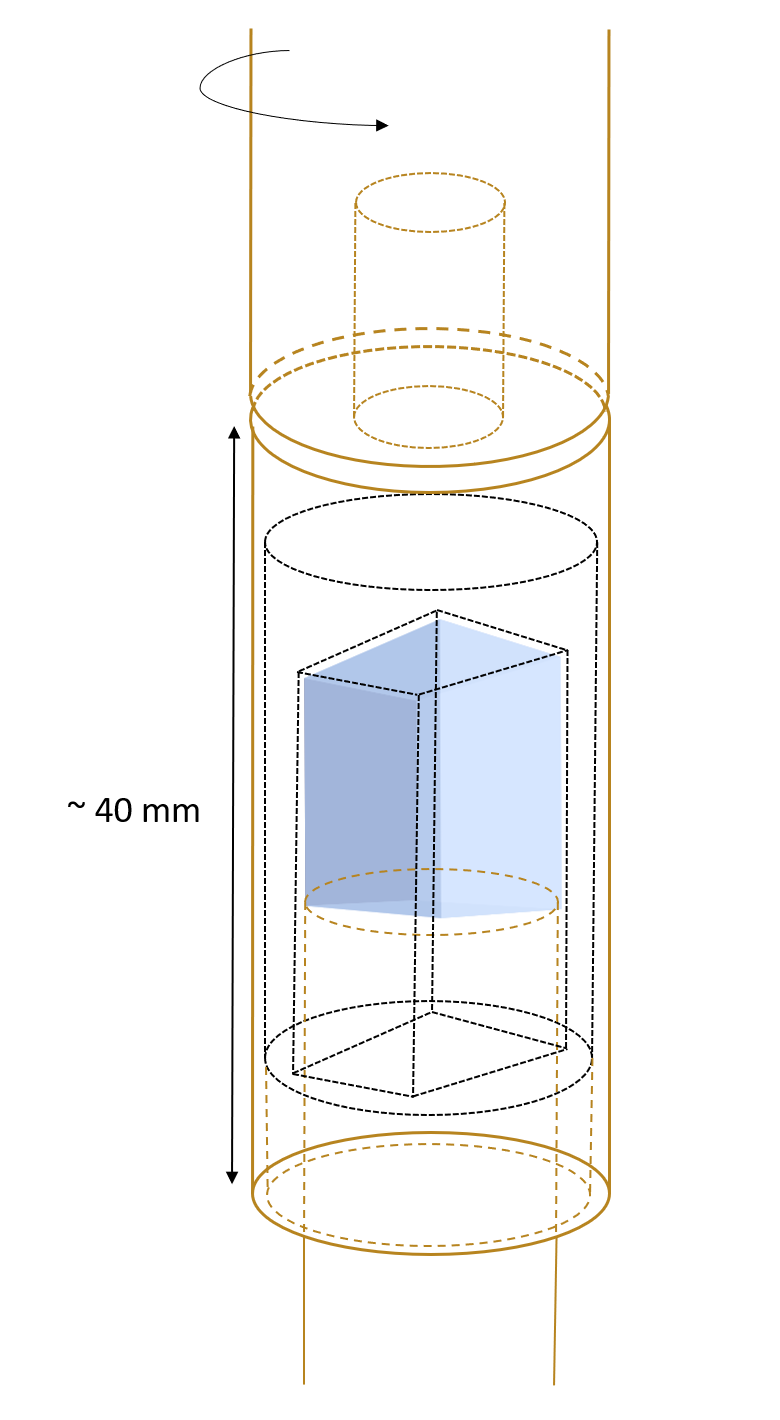
\includegraphics[width=\textwidth]{sampleholder}
       \caption{\label{fig:sampleholder}} 
       \end{subfigure}
%     \hfill
    \begin{subfigure}[b]{0.4\textwidth}
        \centering
        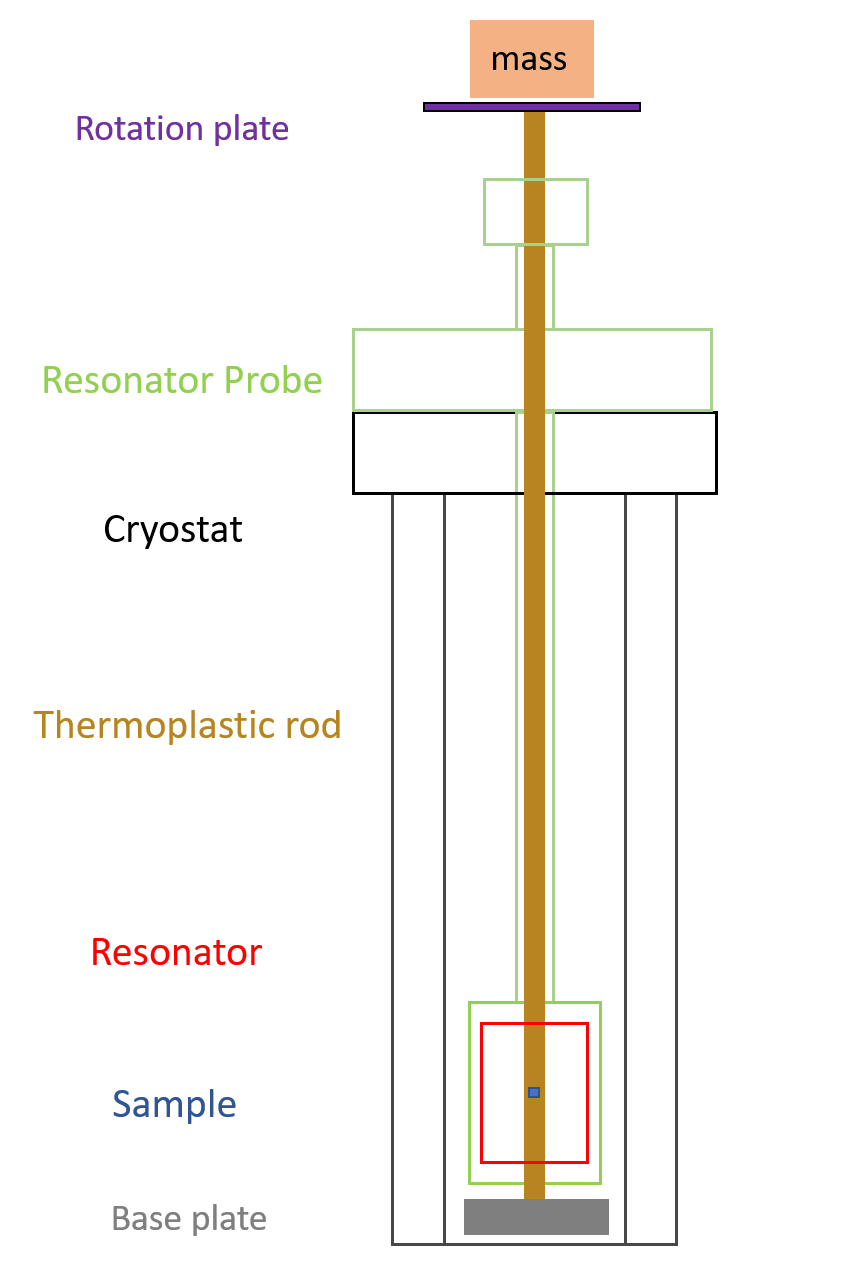
\includegraphics[width=\textwidth]{cryostatschematic}
        \caption{\label{fig:cryostatschematic} }
     \end{subfigure}
    \caption{(a) Illustration of an adapter strain mount for the YSO sample with the b-axis parallel to the rod axis. (b) Schematic of experimental setup showing ESR resonator probe mounted inside liquid Helium flow cryostat. The sample is held in place in the centre of the resonator by fabricated thermoplastic rods.}
\end{figure}

The main thermoplastic rod is connected to the fiberglass rod via a screw. Connection between the adapter and the main rod is obtained by connecting the main thermoplastic piece to the adapter by fabricating a screw and thread. This is done by milling a small recess into to the rod and tapping to create the nut. The adapters are sanded and a die is used to create the bolt. The adapter piece for the sample holder is shown in Fig~\ref{fig:sampleholder} where the cryostat schematic is shown in Fig.~\ref{fig:cryostatschematic}. Similarly a recess is milled in the opposite end of the adapter where, iRoland Modela computer numerical control (CNC) machined, acrylic sample holders are secured within using epoxy resin. To provide further protection against the becoming lost within the cryostat, the new solid thermoplastic piece connected to the base plate is sanded such that it fits within the adapter pieces and thus is secured using cryogenic tape. Therefore, due to do added tape thickness the adapters must be sanded as much as possible to allow free rotation when inside the resonator. Further images of the sample holder and thermoplastic pieces are shown in Appendix~\ref{sec:sampleprobefabrication}.


\subsection{EPR spectrometer}
The EPR spectrometer and MATLAB instrument interface GARII was built by Gary Wolfowicz and further enhanced by Philipp Ross~\citep{mansirthesis}. This device enables AC pulses to be generated which drive transitions between the electron spin states in the sample and additionally to detect the echo signal. The EPR spectrometer schematic is shown in Fig.~\ref{fig:zoidberg}. 

\begin{figure}[h]
\centering
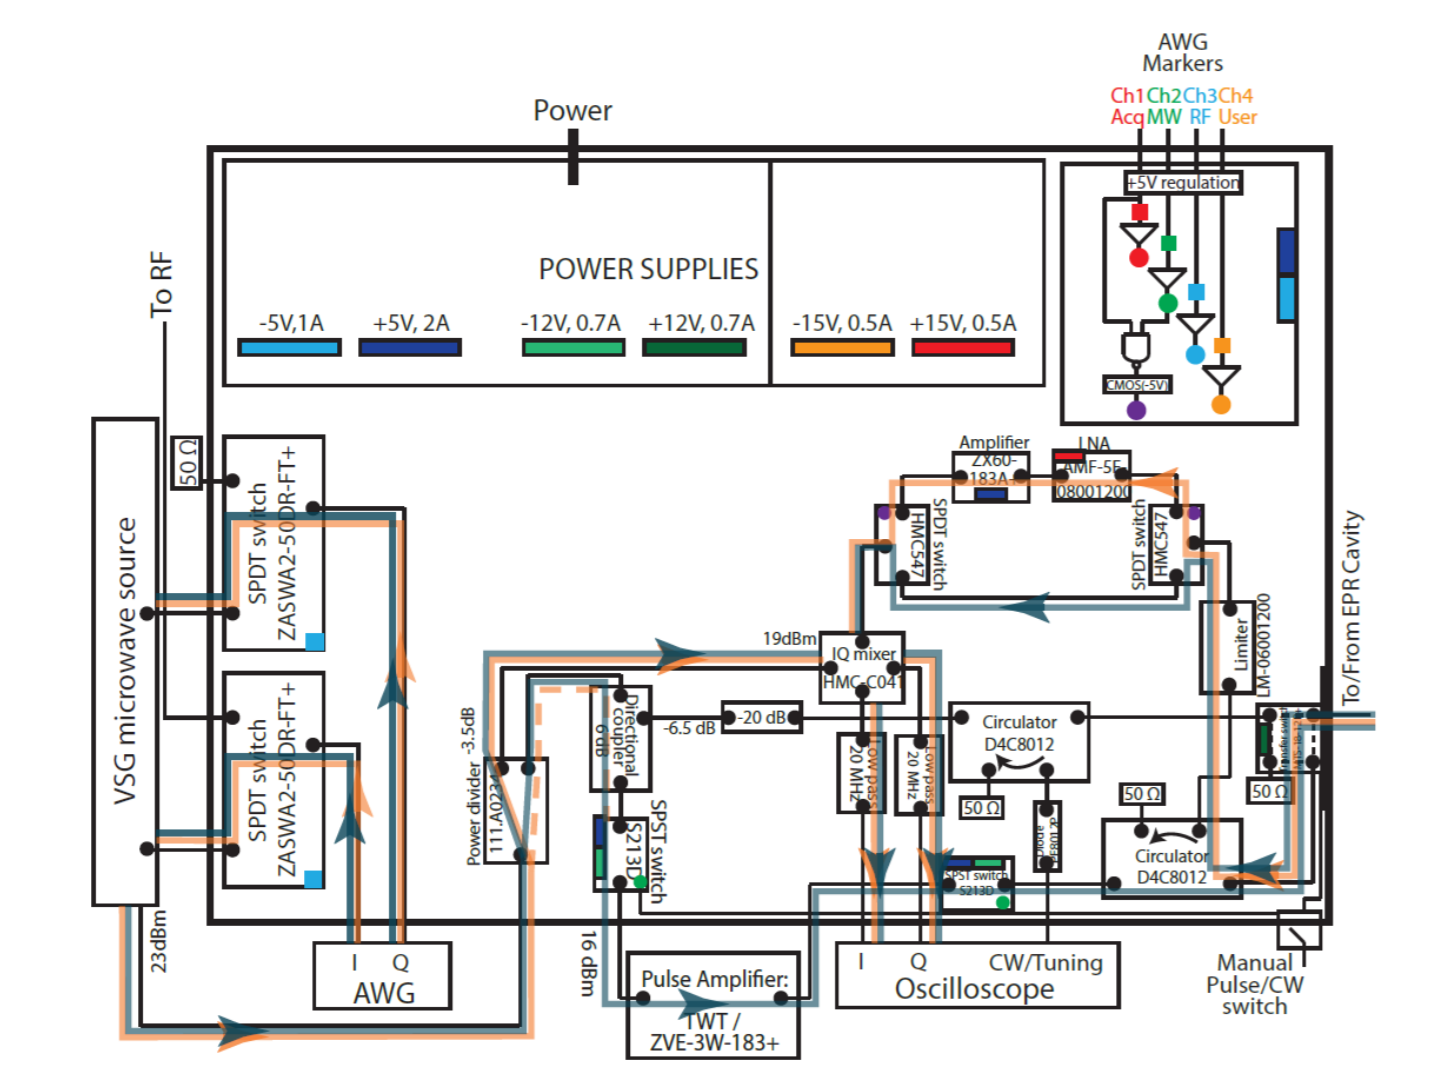
\includegraphics[height=0.5\textwidth,keepaspectratio]{zoidberg}
\caption{\label{fig:zoidberg} EPR spectrometer schematic\citep{mansirthesis}.}
\end{figure}

The $\omega_{MW}$ AC pulse is generated by the vector signal generator (VSG) and modulated using a arbitrary waveform generator. The signal amplitude is controlled by using a TWT amplifier and attenuator. The high power pulse is then sent via the circulator to the coaxial antenna. During the acquisition time window the protection switch is set such that the weak response echo signal is transmitted to the low-noise amplifier (LNA). Therefore during experimental set-up the attenuated must be reduced in integer dB steps whilst and MW pulses are inspected to ensure there is no pulse ringing in the acquisition window as this could damage the sensitive electronic components. The amplified detection signal is then sent to a quadrature mixer with the reference VSG signal where demodulation of the in-phase (I) and out-of-phase (Q) components are displayed by the oscilloscope~\citep{goldfarb2018epr}. 



\section{\label{sec:simulation}Simulation}
The MATLAB toolbox EasySpin was used to simulate the electron paramagnetic spectra used to guide the experimental measurements for this project. Information about the crystal symmetry, the rare-earth ion electron and nuclear spin quantum number the tensors determined by Welinski~\citep{PhysRevB.94.155116}, presented in Section.~\ref{sec:YSOdopedYbions}, was inputted. This allows properties of $^{171}$Yb$^{3+}$:YSO to be probe computationally through the use of spin Hamiltonian solvers. The energy level transitions can be obtained depending on the orientation of the static magnetic field, where the case for $\bm{B_{0}}$ along the D1-axis is shown in Fig~\ref{fig:energylevsim} for each crystal site. 


\begin{figure}[H]
    \centering
    \begin{subfigure}[b]{0.4\textwidth}
        \centering
        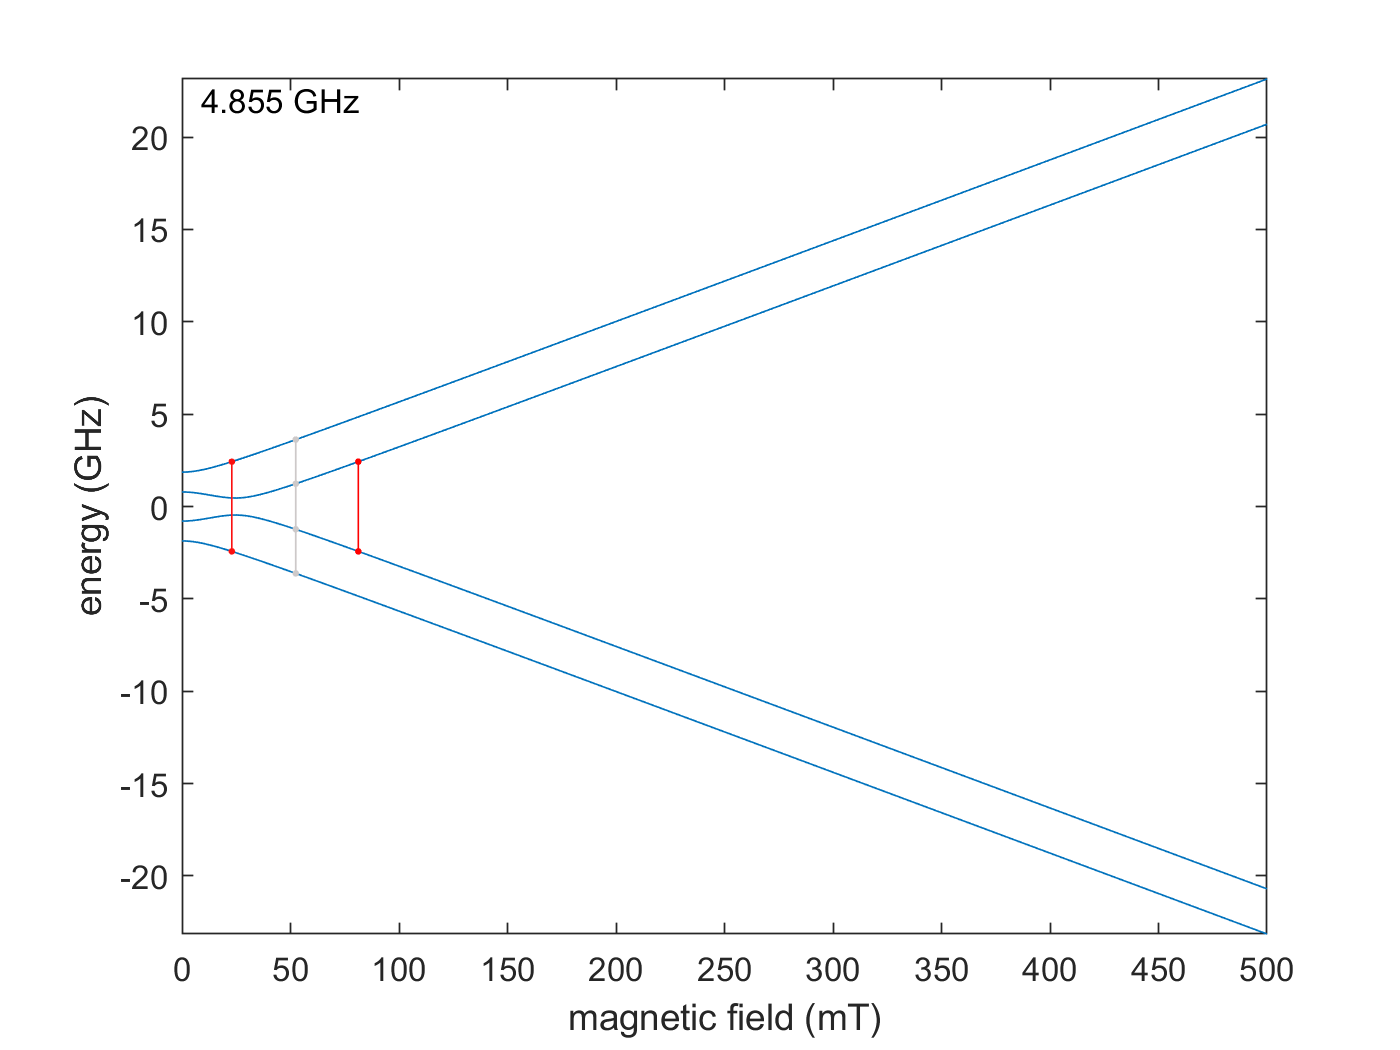
\includegraphics[width=\textwidth]{site1energylevels}
        \caption{}
    \end{subfigure}
%     \hfill
    \begin{subfigure}[b]{0.4\textwidth}
        \centering
        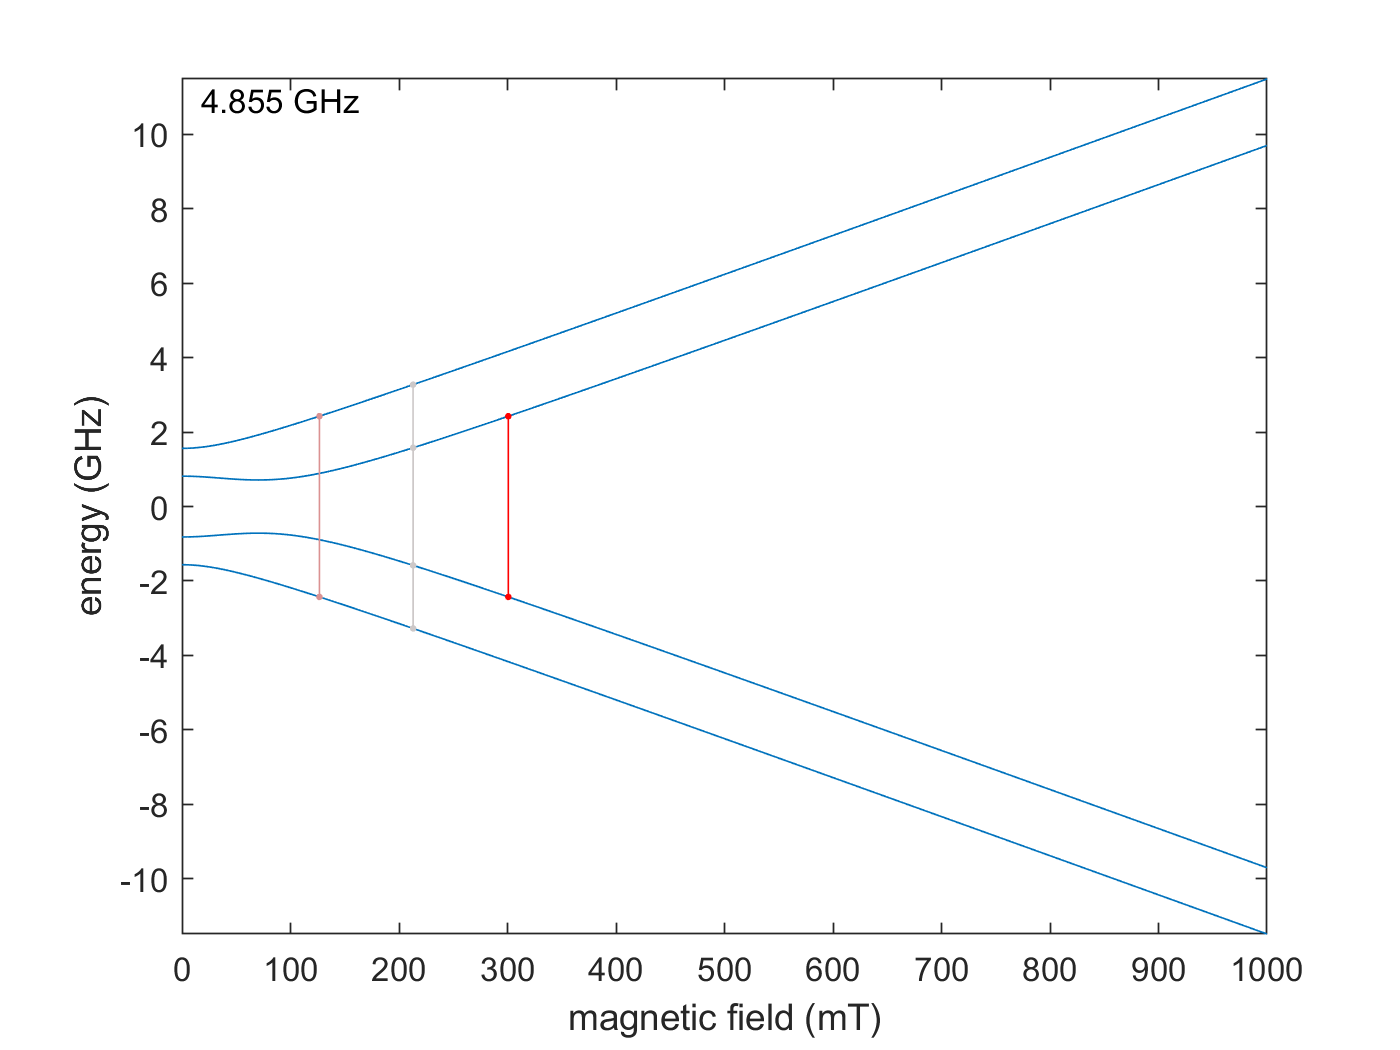
\includegraphics[width=\textwidth]{site2energylevels}
   \caption{}
   \end{subfigure}
   \caption{$^{171}$Yb:YSO energy spectra as a function of the strength of $B_{0}$ along the D1 axis for (a) site I and (b) site II. Transition between allowed (red) and disallowed (grey) eigenstates are shown for a resonator frequency of 9.63 GHz.}
   \label{fig:energylevsim}
\end{figure}


\begin{figure}[H]
    \centering
    \begin{subfigure}[b]{0.46\textwidth}
        \centering
        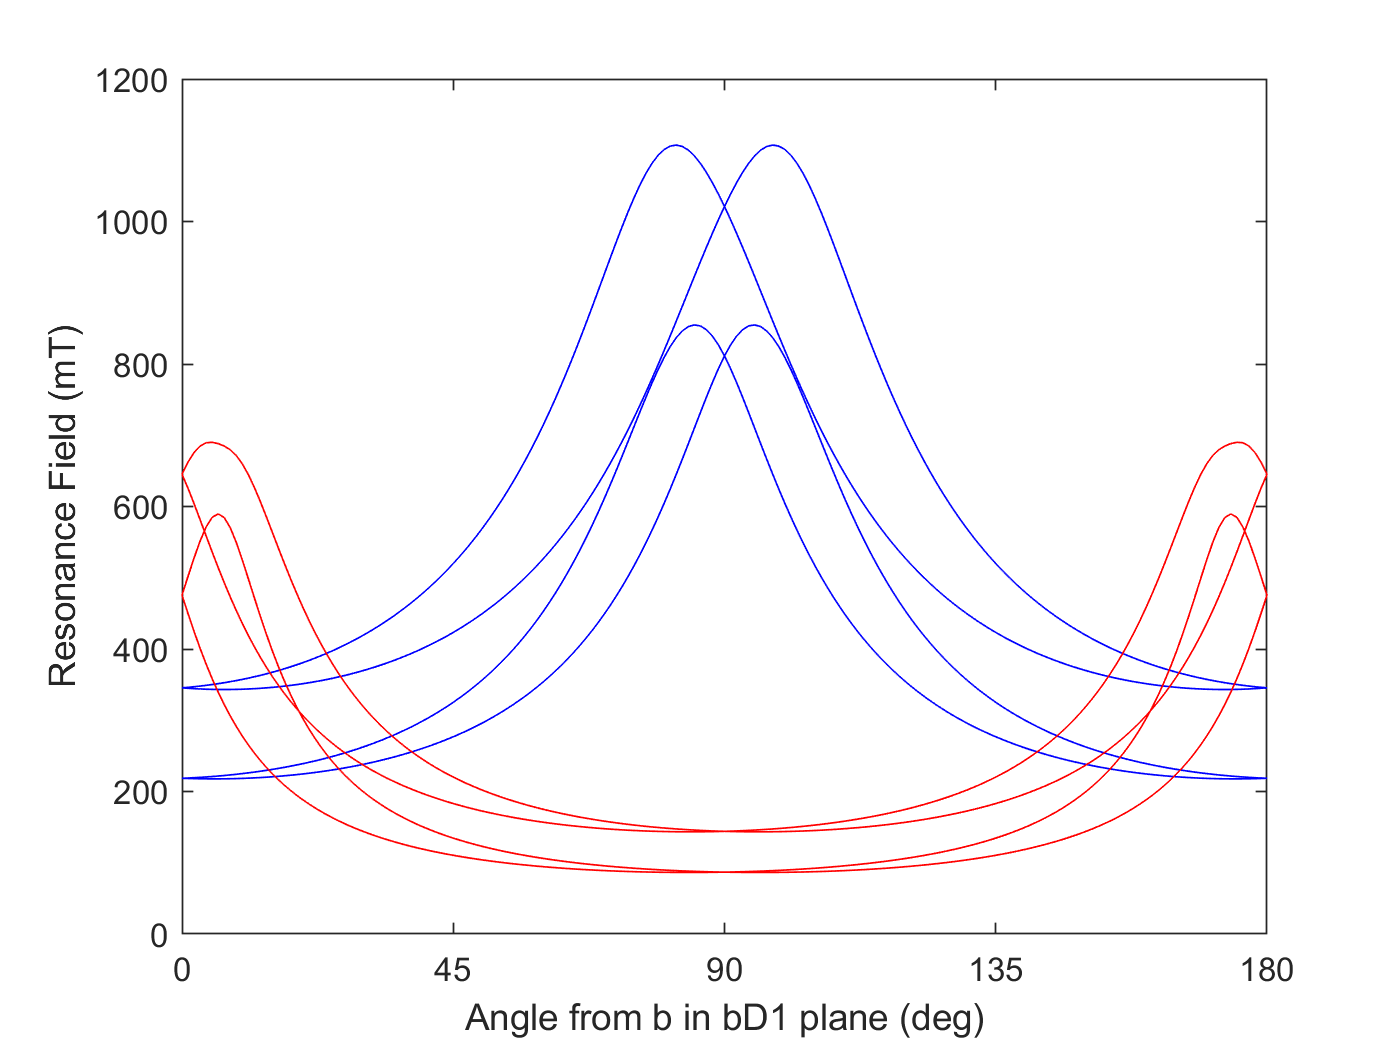
\includegraphics[width=\textwidth]{frombinbD1plane}
        \caption{\label{fig:simmagresori1}}
    \end{subfigure}
%     \hfill
    \begin{subfigure}[b]{0.3\textwidth}
        \centering
        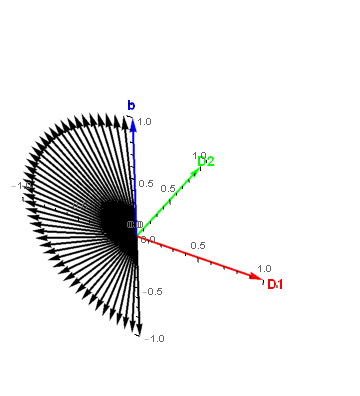
\includegraphics[width=\textwidth]{BperD2}
   \caption{}
   \end{subfigure}
       \begin{subfigure}[b]{0.46\textwidth}
        \centering
        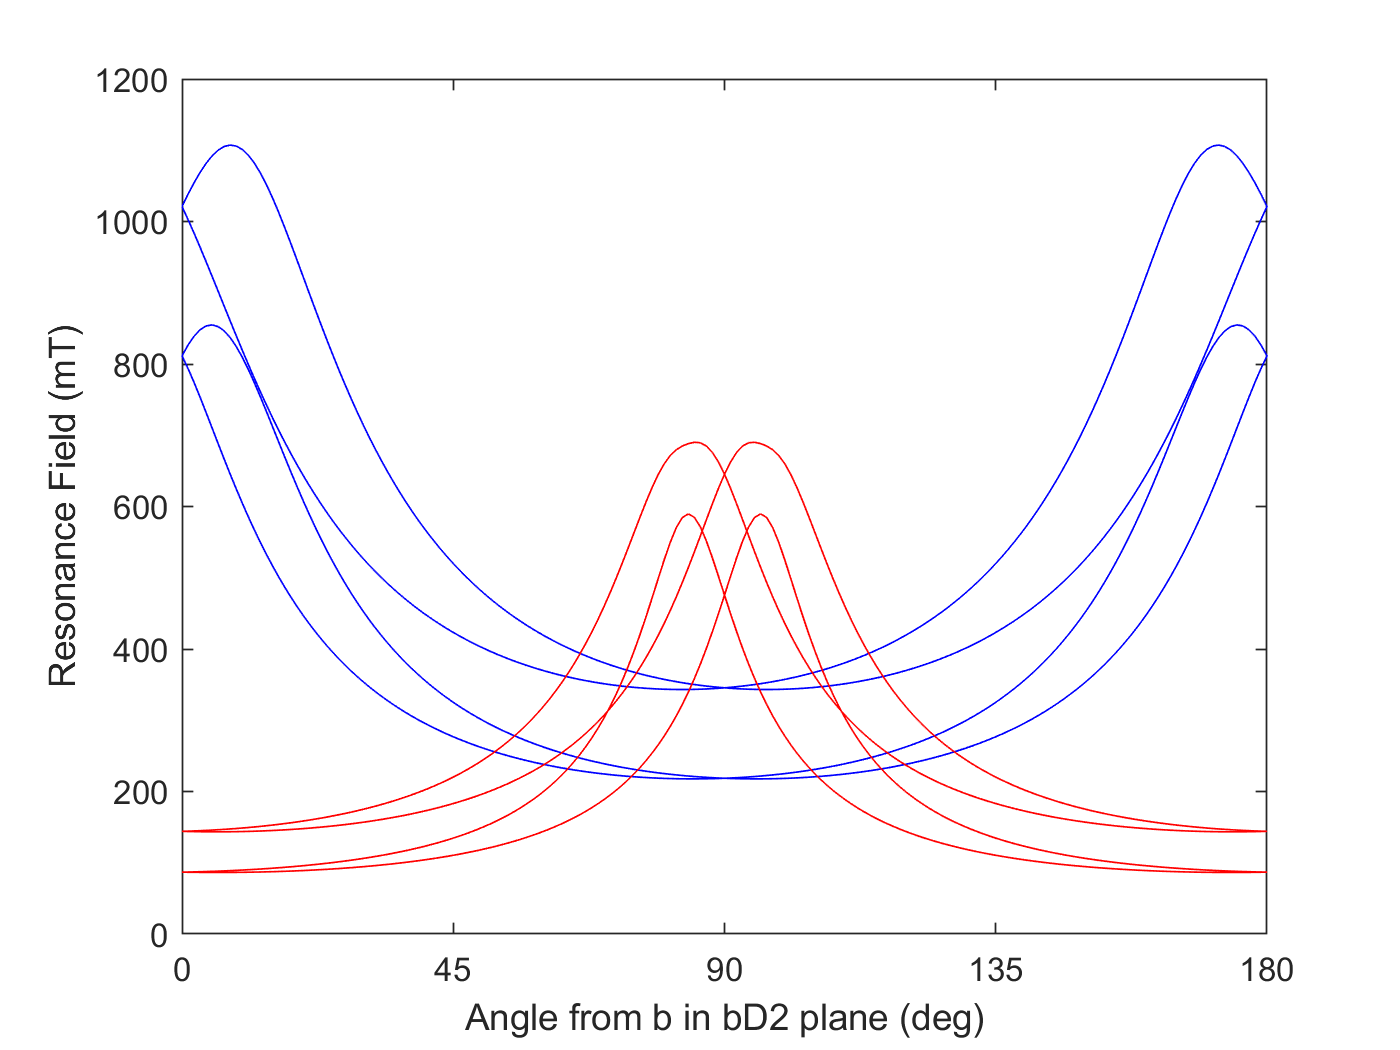
\includegraphics[width=\textwidth]{frombinbD2plane}
   \caption{\label{fig:simmagresori2}}
   \end{subfigure}
       \begin{subfigure}[b]{0.3\textwidth}
        \centering
        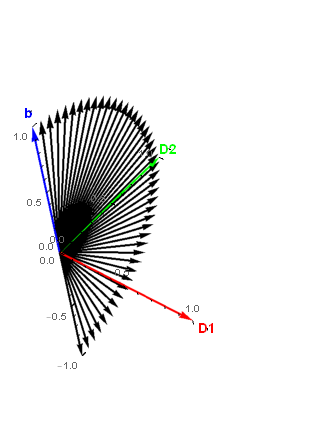
\includegraphics[width=\textwidth]{BperpD1}
   \caption{}
   \end{subfigure}
       \begin{subfigure}[b]{0.46\textwidth}
        \centering
        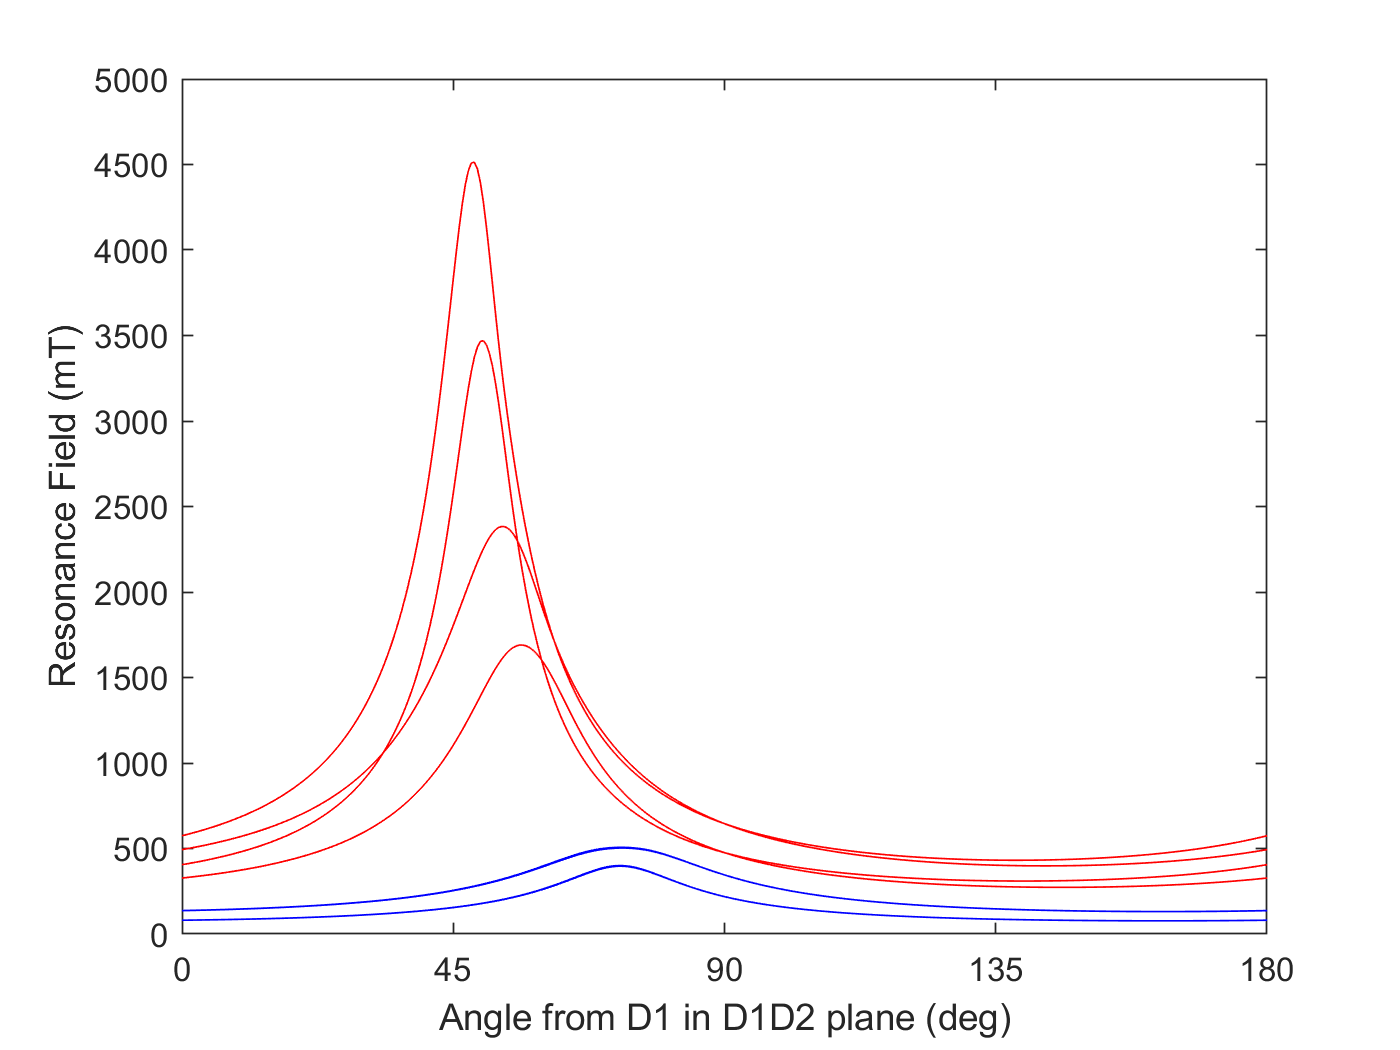
\includegraphics[width=\textwidth]{fromD1inD1D2plane}
   \caption{\label{fig:simmagresori3}}
   \end{subfigure}
       \begin{subfigure}[b]{0.3\textwidth}
        \centering
        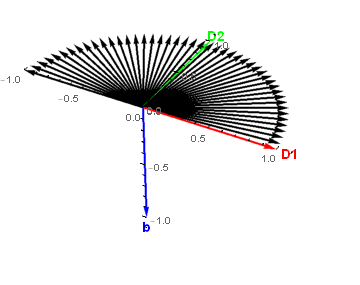
\includegraphics[width=\textwidth]{Bperb}
   \caption{}
   \end{subfigure}
   \caption{The resonant magnetic field for $^{171}$Yb:YSO as a function of orientation is shown in (a),(c) and (e) where magnetic field relative to the dielectric axes is displayed in (b),(d) and (f), respectively. Site I is shown in blue and site II is shown in red.}
   \label{fig:simmagresori}
\end{figure}

To investigate the resonant magnetic field as a function of the orientation of the sample I firstly, as shown in Appendix~\ref{sec:easyspinsim}, reproduced the results in Ref.~\citep{mairflaig} for $145$Nd$^{3+}$ doped YSO. Thereafter, the magnetic field resonance vs. orientation is computed which is good agreement with the experimentally measured values in Ref.~\citep{PhysRevB.94.155116}. The sub-site magnetic field degeneracies are lifted as the orientation is varied as shown in Fig.~\ref{fig:simmagresori}. To obtain magnetic field splitting for Fig~\ref{fig:simmagresori3} a small $R_{y}$ rotation of the initial magnetic field vector is included since there is a small error ($\approx$2$^{\circ}$) is associated with cutting the sample along the dielectric axes~\citep{PhysRevB.94.155116}.    


\begin{figure}[H]
    \centering
    \begin{subfigure}[b]{0.45\textwidth}
        \centering
        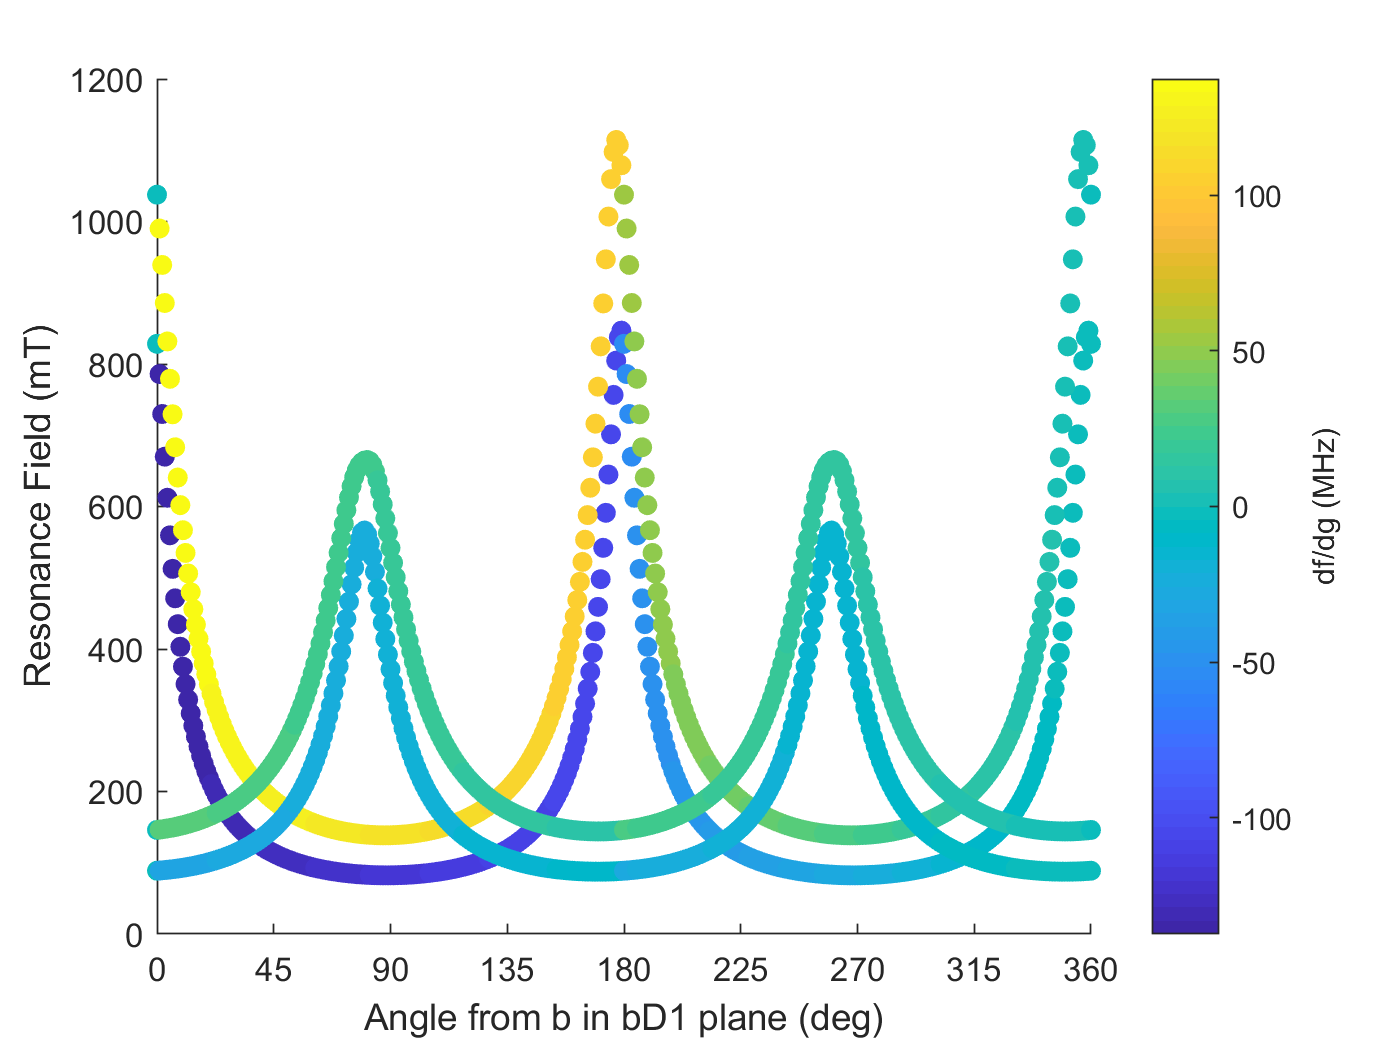
\includegraphics[width=\textwidth]{pertanglebinbD1plane}
        \caption{\label{fig:simmagresori1}}
    \end{subfigure}
%     \hfill
    \begin{subfigure}[b]{0.45\textwidth}
        \centering
        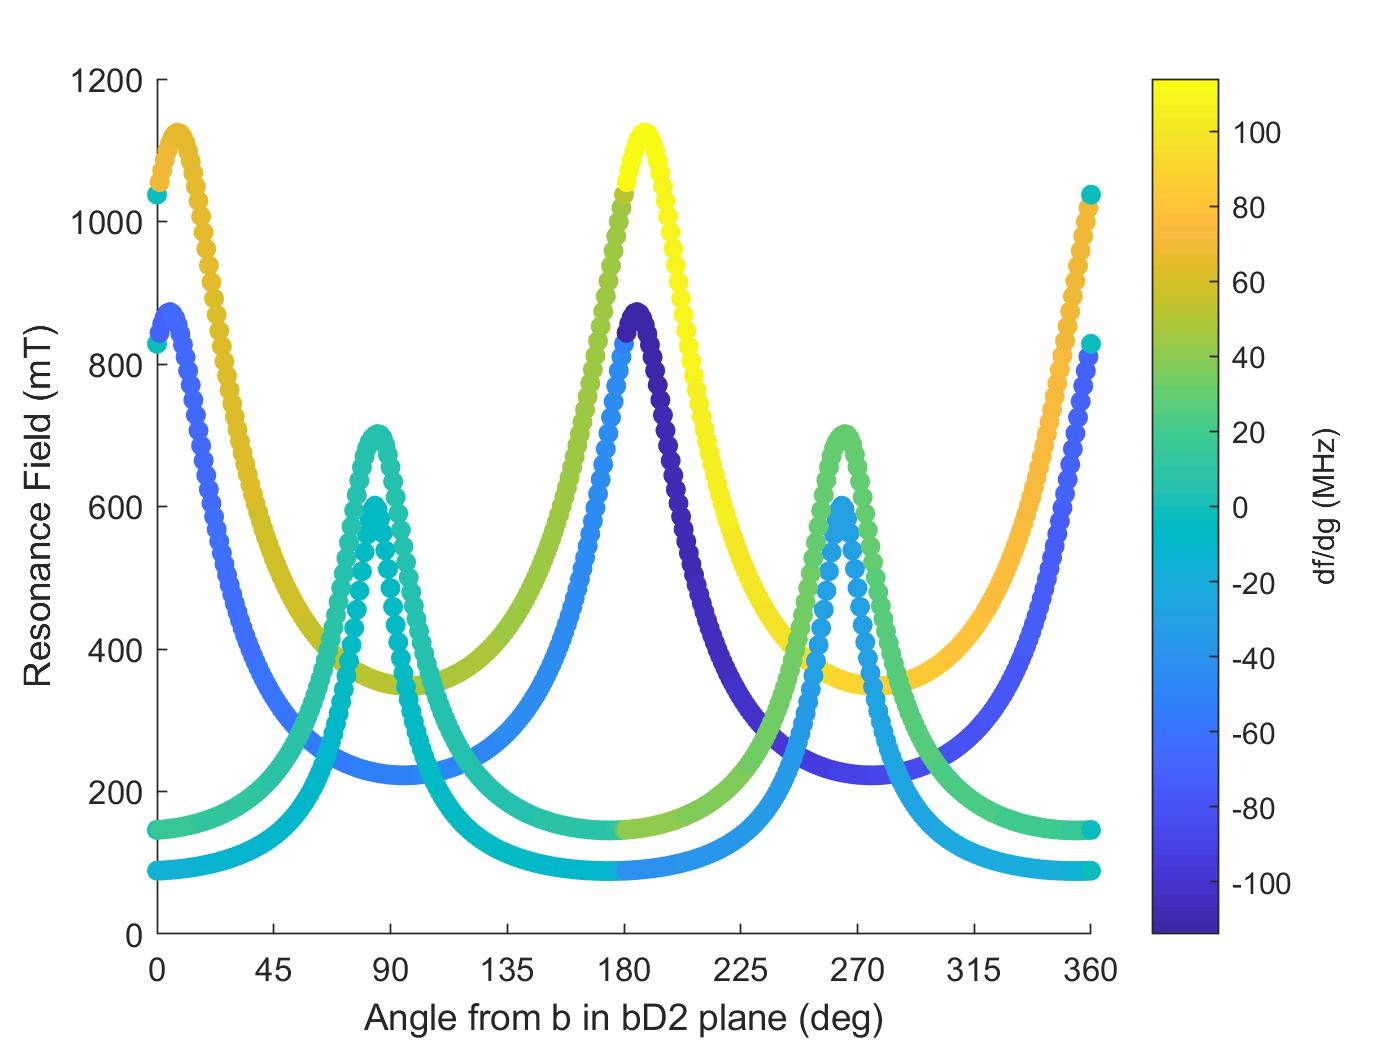
\includegraphics[width=\textwidth]{pertanglebinbD2plane}
   \caption{}
   \end{subfigure}
       \begin{subfigure}[b]{0.45\textwidth}
        \centering
        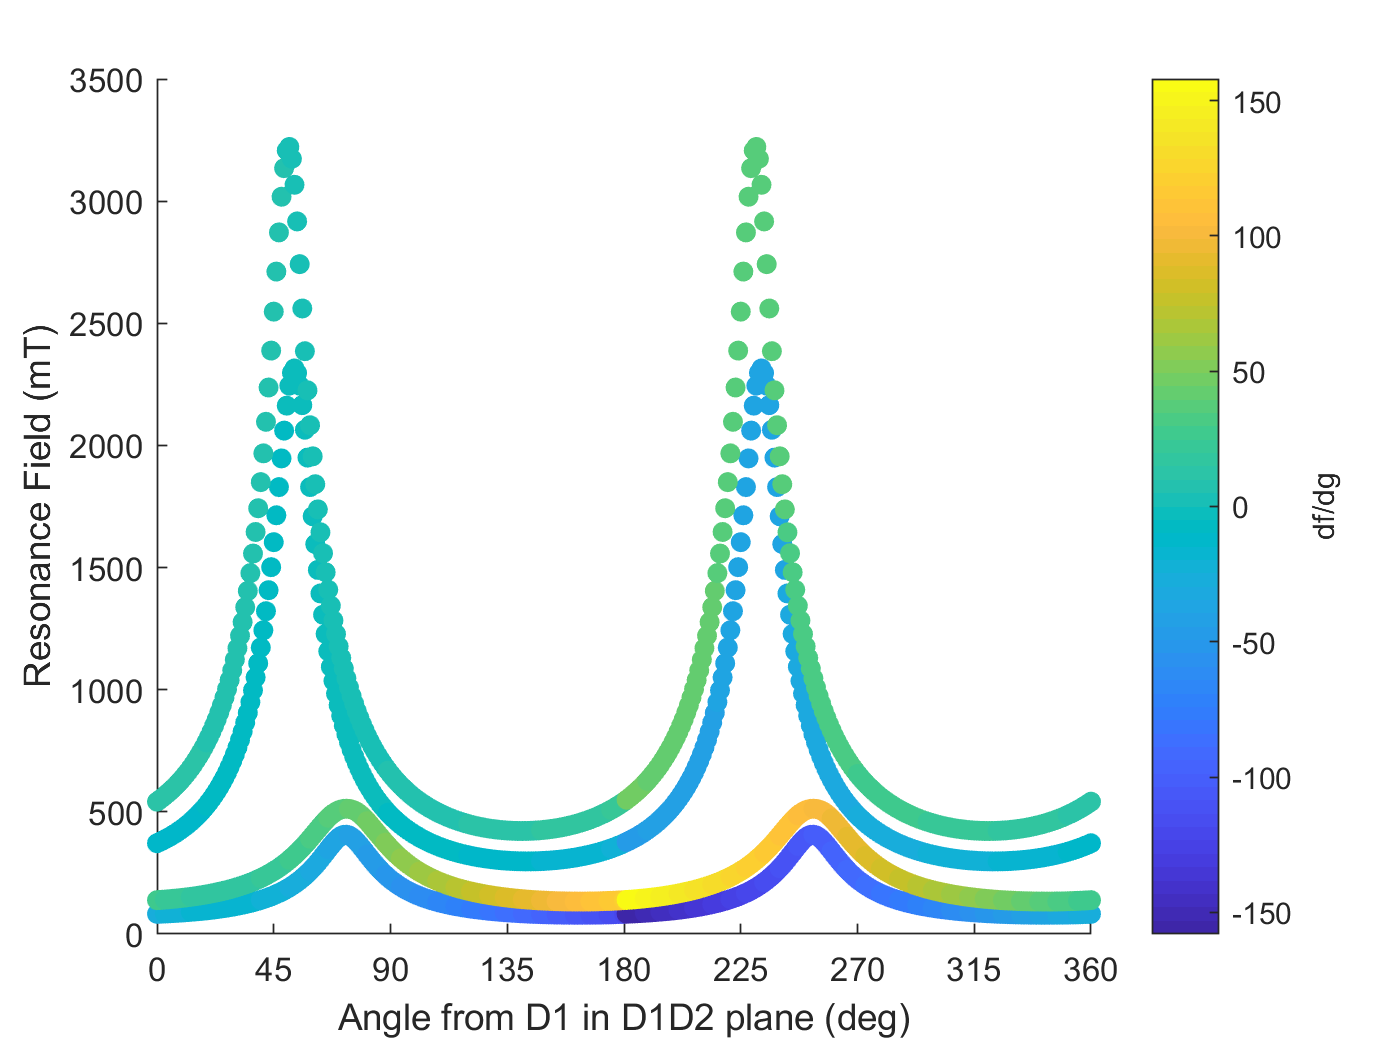
\includegraphics[width=\textwidth]{pertangleD1inD1D2plane}
   \caption{\label{fig:simmagresori2}}
   \end{subfigure}
   \caption{Angular variations of the EPR transitions for $^{171}$Yb:YSO where the colour bar represents $\Delta f/\Delta g$ for isotropic $\Delta g = 0.05$. Where $\bm{B_{0}}$ is perpendicular to the (a) D2-axis, (b) D1-axis and the (c) b-axis.}
   \label{fig:dfdg}
\end{figure}


\begin{figure}[H]
    \centering
    \begin{subfigure}[b]{0.45\textwidth}
        \centering
        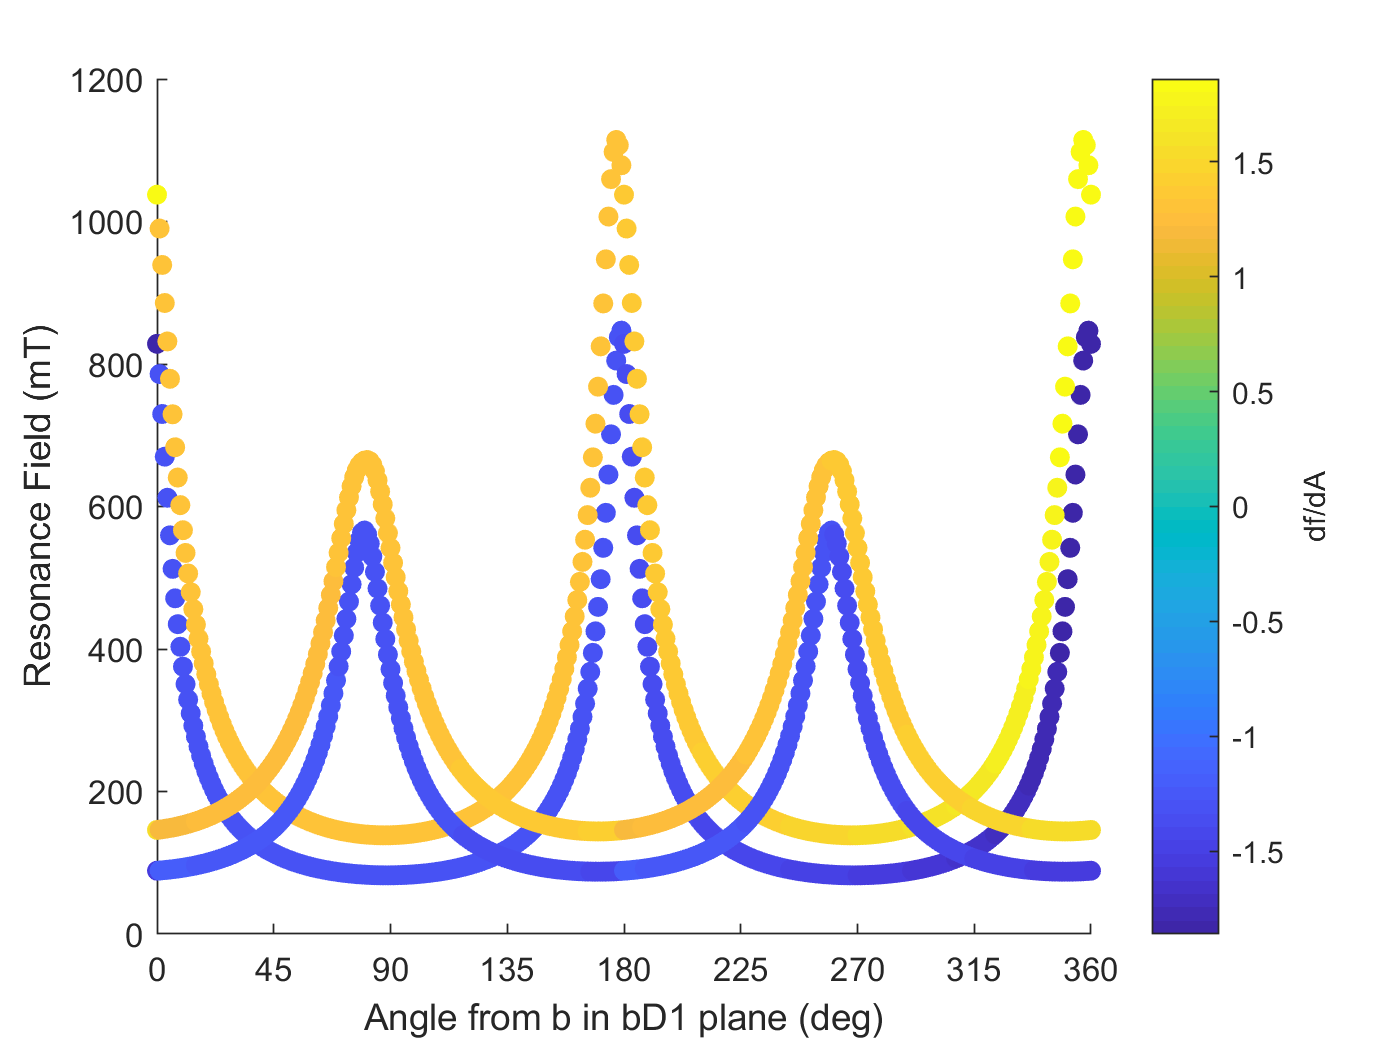
\includegraphics[width=\textwidth]{pertAanglebinbD1plane}
        \caption{\label{fig:simmagresori1}}
    \end{subfigure}
%     \hfill
    \begin{subfigure}[b]{0.45\textwidth}
        \centering
        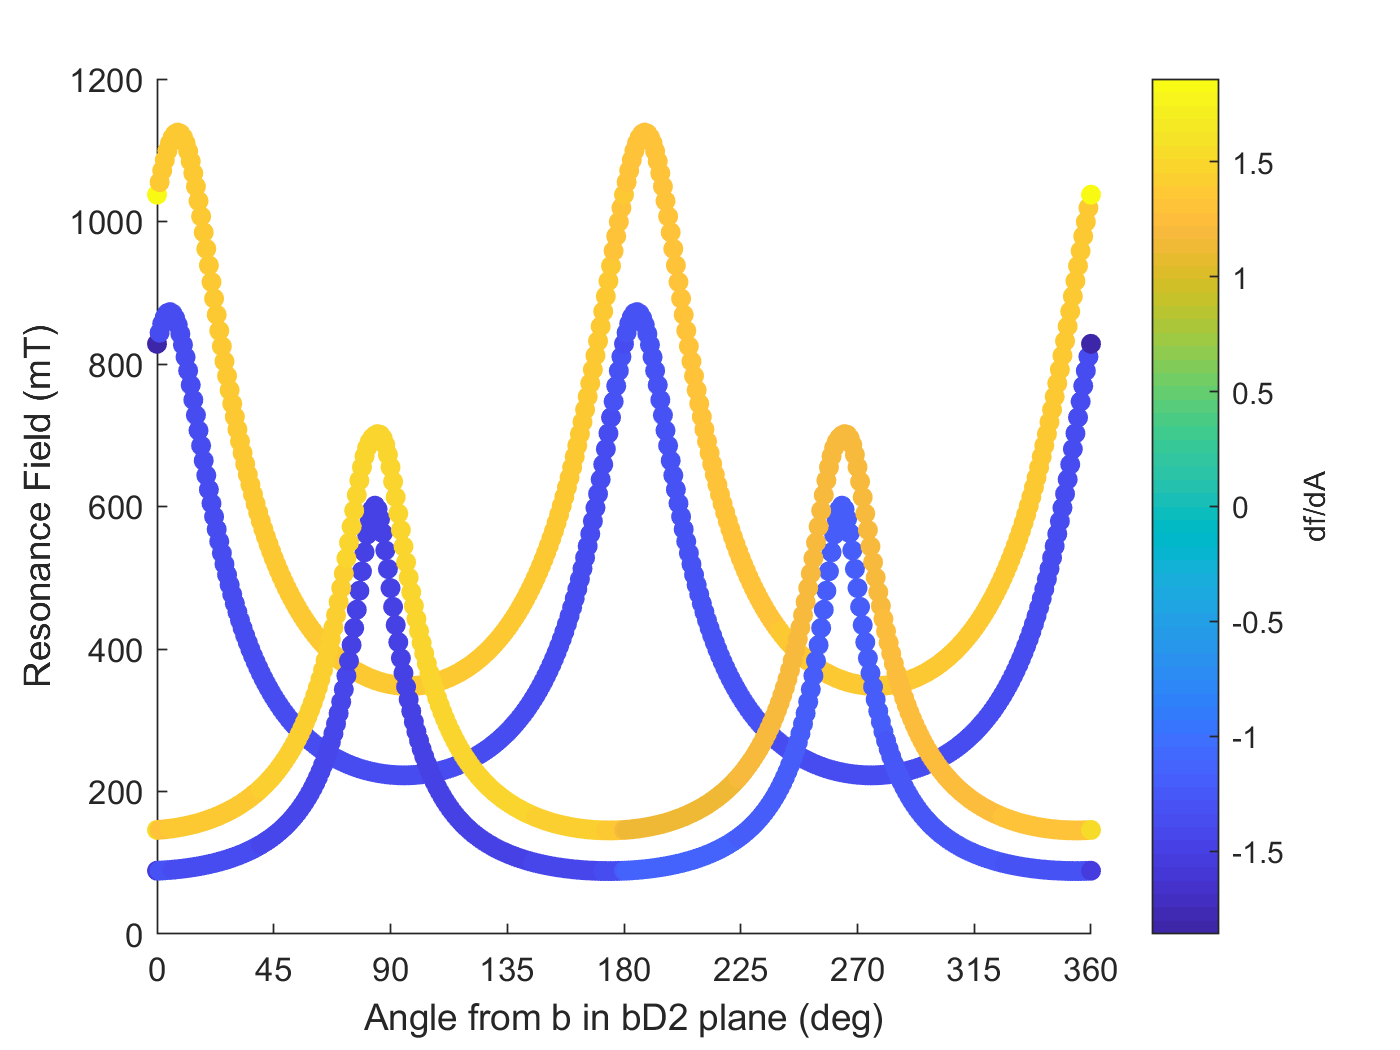
\includegraphics[width=\textwidth]{pertAanglebinbD2plane}
   \caption{}
   \end{subfigure}
       \begin{subfigure}[b]{0.45\textwidth}
        \centering
        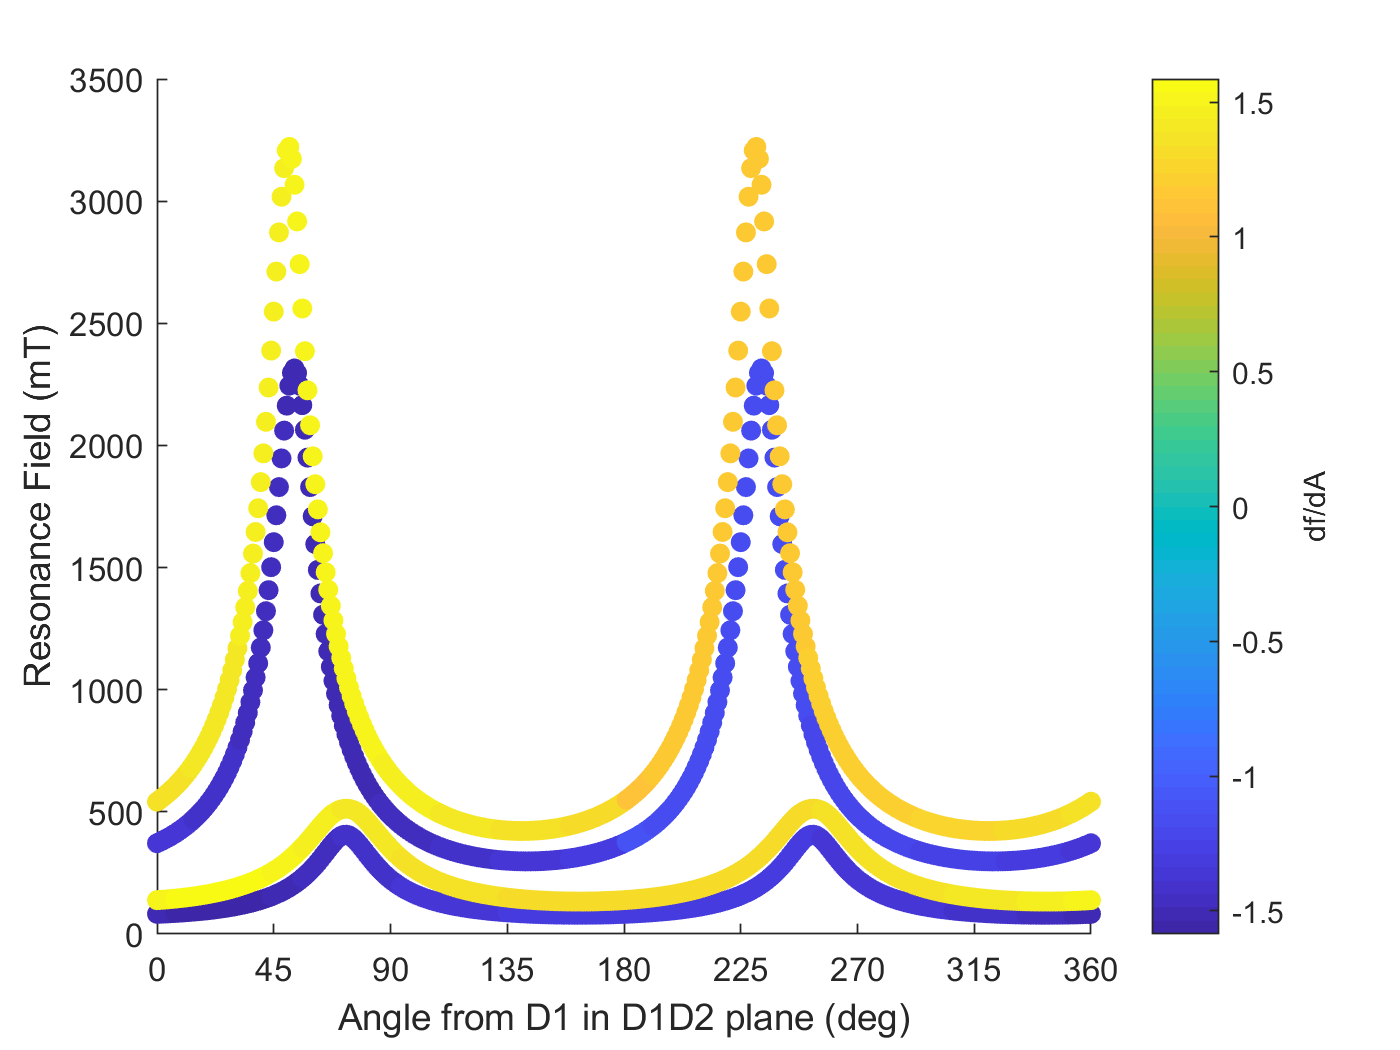
\includegraphics[width=\textwidth]{pertAangleD1inD1D2plane}
   \caption{\label{fig:simmagresori2}}
   \end{subfigure}
   \caption{Angular variations of the EPR transitions for $^{171}$Yb:YSO where the colour bar represents $\Delta f/\Delta A$ for isotropic $\Delta A = 50$ MHz. Where $\bm{B_{0}}$ is perpendicular to the (a) D2-axis, (b) D1-axis and the (c) b-axis.}
   \label{fig:dfdA}
\end{figure}

Furthermore, the calculated change in resonance frequency, $\Delta f$ in response to a small perturbation of either $\bm{g}$ and $\bm{A}$ was explored. The case of an isotropic perturbation of $\Delta g = 0.05$ and $\Delta A = 50$ MHz for each site is shown in Fig.~\ref{fig:dfdg} and Fig.~\ref{fig:dfdA}, respectively. This case simulates the expected effect of isotropic strain. Additionally cases of uniaxial perturbation of $\bm{g}$ and $\bm{A}$ were simulated. However, in reality due the number of nonzero stiffness matrix terms of YSO and unknown $\bm{\mathcal{G}}$ and $\bm{\mathcal{A}}$ tensors, the response of $\bm{g}$ and $\bm{A}$ to uniaxial strain in YSO remains undisclosed. Therefore these simulations provide a preliminary guidance of which crystal orientation to probe.





%This research aims to provide a companion to the investigation of the effect of mechanical strain applied to a group V doped $^28$Si presented in Ref.~\citep{doi:10.1063/1.4919761}. 

    \chapter{Results}
This section details the experimental results of investigating the effect of strain in $^{171}$Yb doped YSO. Following each cool down and prior to any pulse measurement the centre frequency $f_{c}$ of the cavity is obtained in tunning mode. Tunning mode is the safety setting in which the signal always bypasses the LNA. The cavity resonance is differentiated from electronic reflections by tunning the cavity Q factor and observing which absorption peak changes in width. The VSG is set such that the output pulse is resonant with $f_{c}$, where $f_{c}\approx 6.3$ GHz. The Q factor is tuned as required. Thereafter, in pulse mode the attenuation of the input is slowly decreased whilst the ensuring there is no pulse ringing in the acquisition window. 


\section{EPR setup testing}
Following the re-installment of EPR equipment a Gauss meter, measuring up to 30 mT, was used to test the accuracy of the low magnetic fields generated by the field controller. To test the functionality of the setup, EPR spectroscopy of a P doped isotropically purified $^{28}$Si sample was initially completed at 9 K. The strength of echo signal above the noise floor for this sample reduced the difficulty of finding the resonance field for a transition. However, for a Rabi pulse sequence, where the initial pulse duration was swept, the signal amplitude never recovered to complete Rabi oscillations as shown in Fig.~\ref{fig:rabisi28}. Regardless of the settings of the pulse sequence and acquisition time the oscillations were not observed. Additionally a significantly shorter $T_{1}$ time of the order of ns was obtained whilst previous experimental measurements the longitudinal electron spin relaxation time determined this should be of the order of ms~\citep{PhysRevB.68.193207}.  

\begin{figure}[H]
    \centering
    \begin{subfigure}[b]{0.45\textwidth}
        \centering
        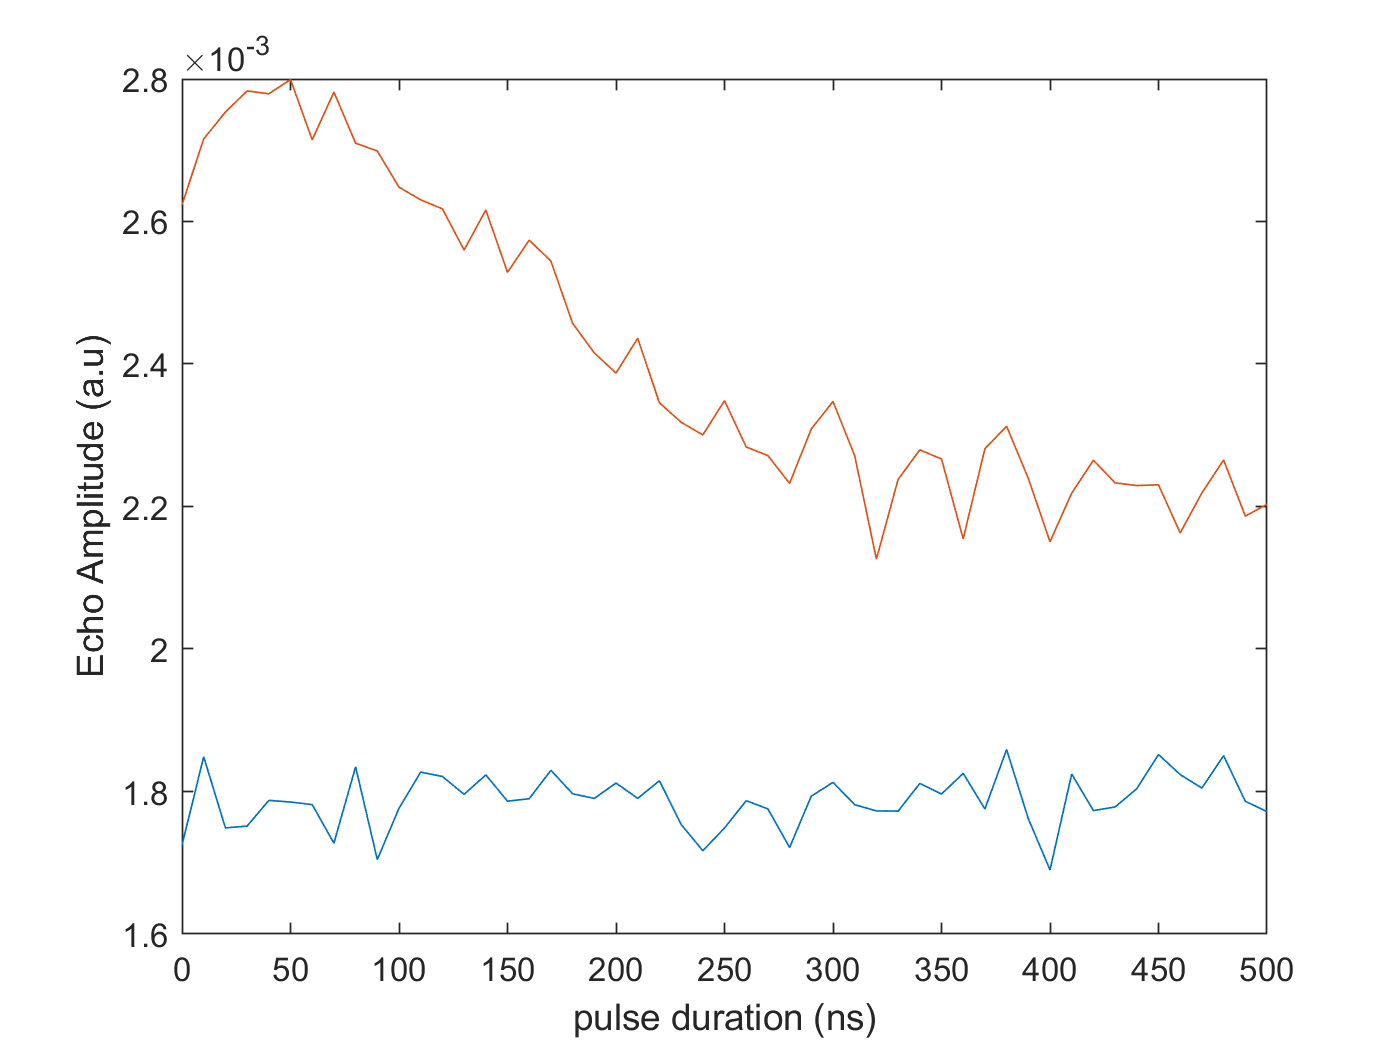
\includegraphics[width=\textwidth]{rabisi28}
        \caption{\label{fig:rabisi28}}
    \end{subfigure}
%     \hfill
    \begin{subfigure}[b]{0.45\textwidth}
        \centering
        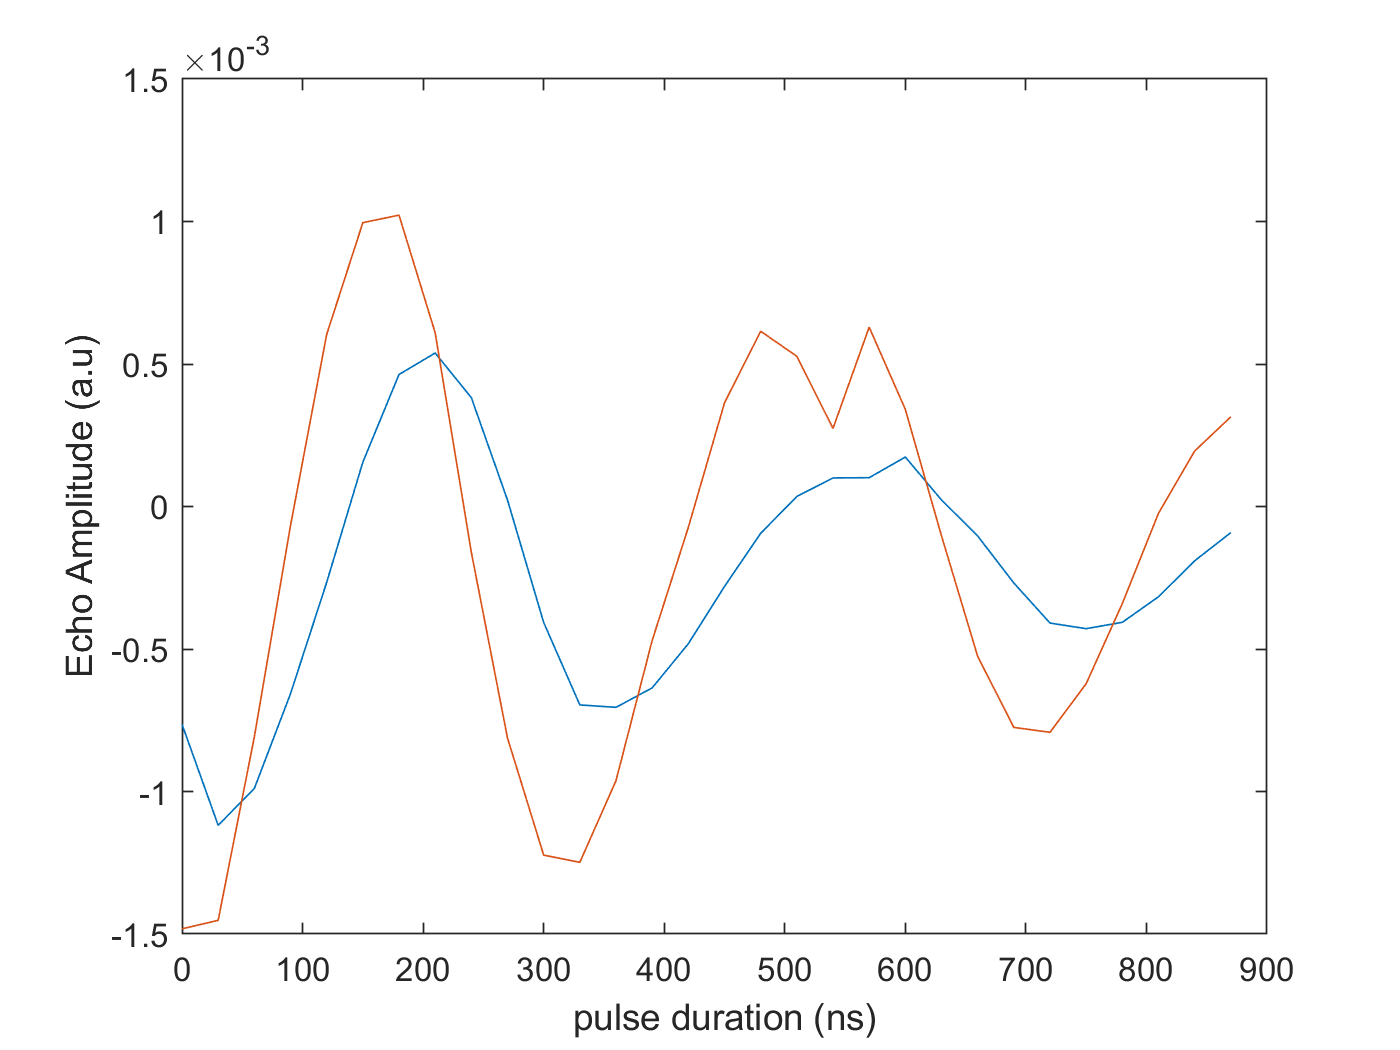
\includegraphics[width=\textwidth]{rabisinatural}
   \caption{\label{fig:rabisinatural}}
   \end{subfigure}
    \caption{Response to rabi pulse sequence of (a) $^28$Si doped with P and (b) natural Si doped P. The in-phase (I) and out-of-phase (Q) signals are shown in blue and red, respectively.}
\end{figure}

Due to concern that the issue was the significant fluctuations of the magnetic field during measurement since the field controller is normally constantly left running provide the most stable field, the sample was switched to a natural Si sample. The contribution of the $^{29}$Si nuclear spins results in dephasing which broadens the resonance linewidth~\citep{Hileeaaq1459}. The Rabi oscillations obtained for the natural Si sample is shown in Fig.~\ref{fig:rabisinatural}. An inversion recovery pulse sequence was completed to determine $T_{1}$ of $\approx 20$ ms.    

\section{$^{171}$Yb$^{3+}$:YSO EPR spectra}
The $^{171}$Yb$^{3+}$:YSO is then placed into the cryostat in approximate orientation of $B_{0}\parallel D1$ (or anti-parallel) in the $D1D2$ plane. The EPR transitions are probed at 7 K by sweeping the magnetic field sweeping based on the expected magnetic field resonance given in Fig.~\ref{fig:simmagresori3}. The linewidth of the site I and site II transitions are given as 3.4 mT and 0.1 mT~\citep{PhysRevB.97.064409}. The Q-factor of $\approx$385 is set to provide low energy damping but with a large enough frequency bandwidth to excite the spins. Upon detection of a site II echo pulse, similarly the Rabi experiment is completed to obtain for the amplitude of the AC signal used the optimum pulse duration of $\approx$70 ms to produce a $\pi$ rotation. 

The inversion recovery pulse sequence obtains $T_{1}\approx$2.6 ms which is in good agreement with the expected value at 7 K given in Fig.~\ref{fig:spinrelaxation}. $T_{2}$ is measured as $\approx 9$ $\mu$s using the Hahn echo detection pulse scheme. The measured echo signal for each of the three experiments is given in Appendix~\ref{sec:additionalresults} which is considerably more noisy than in Fig.~\ref{fig:rabisi28} and Fig.~\ref{fig:rabisinatural} due having to remove averaging of the echo signal due to this causing the oscilloscope to continually become unresponsive. However single-shot echo detection, as shown in Fig.~\ref{fig:cleanecho} is adequate for the purposes of this experiment. 

\section{\label{sec:strainexp}$^{171}$Yb$^{3+}$:YSO strain investigation}

Initially the strategy to investigate the effect of strain was to measure the Hahn echo signals whilst increasing mass is placed on top of the sample, applying unaxial stress along the b-axis. The shift in the resonance frequency can then be extracted by fitting to the echo represented in Fourier space~\citep{PhysRevLett.120.167701}. However, upon testing this method concerning observation was made, when a mass was placed on the rotation plane the echo signal completely vanished regardless of the mass used. Therefore, it was clear the shift in the resonance was the result of another mechanism determined to be crystal rotation. Due to the measured sensitivity of the magnetic field resonances to angular rotation of the crystal. The crystal was purposefully rotated 40$^{\circ}$ to approximately 140$^{\circ}$ or 320$^{\circ}$ as shown in Fig.~\ref{fig:site2D1inD1D2plane} (and Fig.~\ref{fig:site2D1inD1D2plane}). However, even for this crystal orientation the sensitivity to a small ($\approx 1-2^{\circ}$) rotation results in a significant shift of the resonance transition. 

\begin{figure}[H]
    \centering
    \begin{subfigure}[b]{0.45\textwidth}
        \centering
        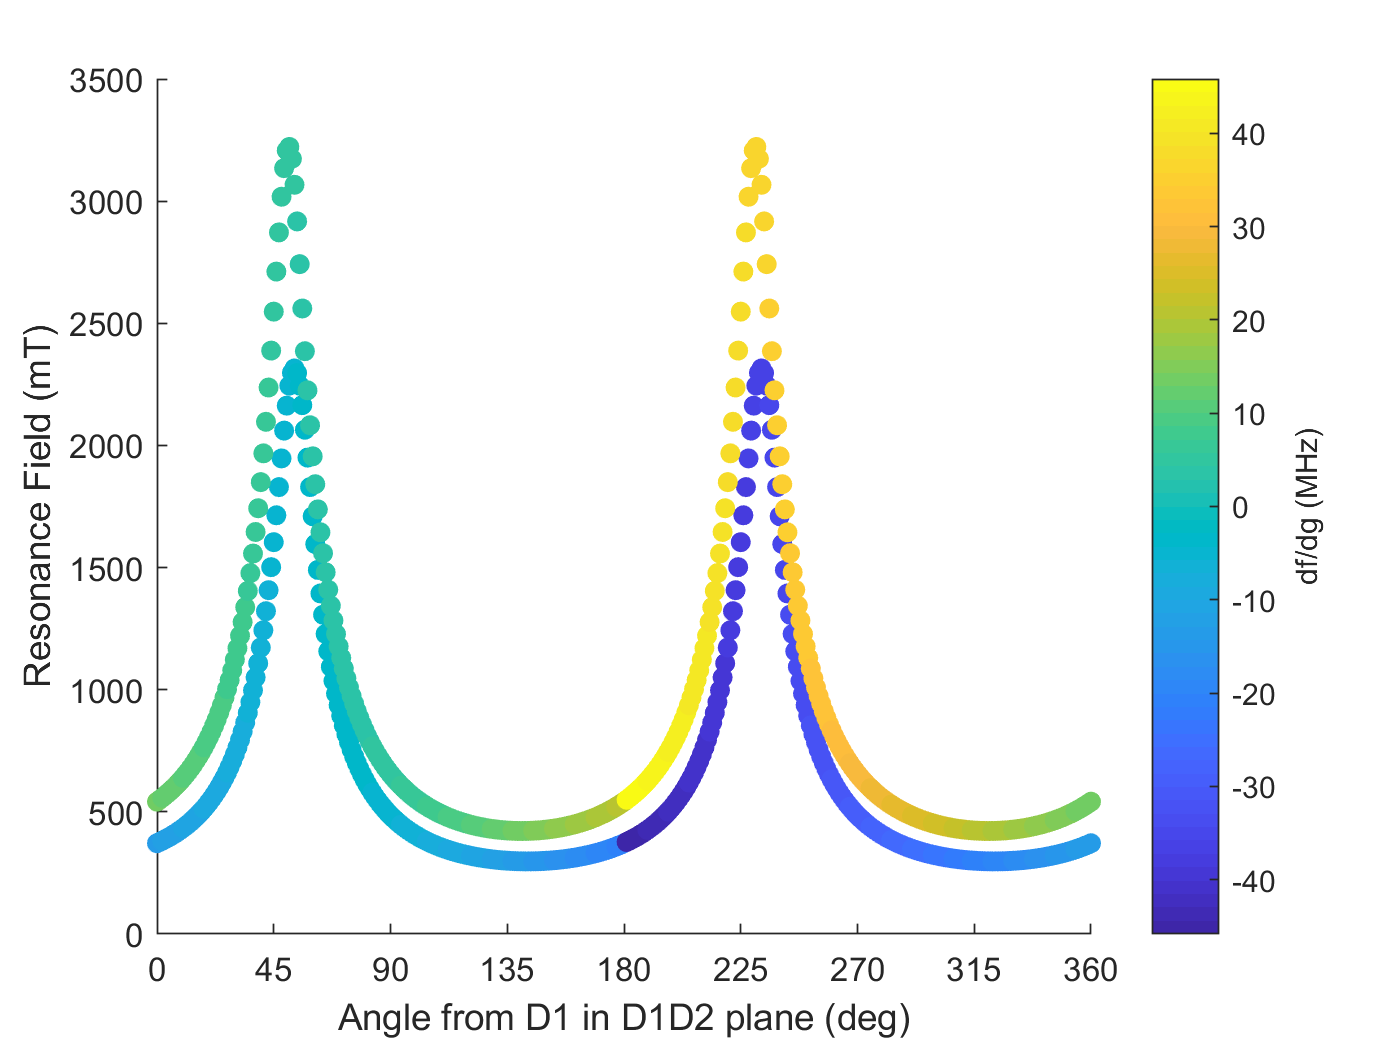
\includegraphics[width=\textwidth]{site2D1inD1D2plane}
        \caption{\label{fig:site2D1inD1D2plane}}
    \end{subfigure}
%     \hfill
    \begin{subfigure}[b]{0.45\textwidth}
        \centering
        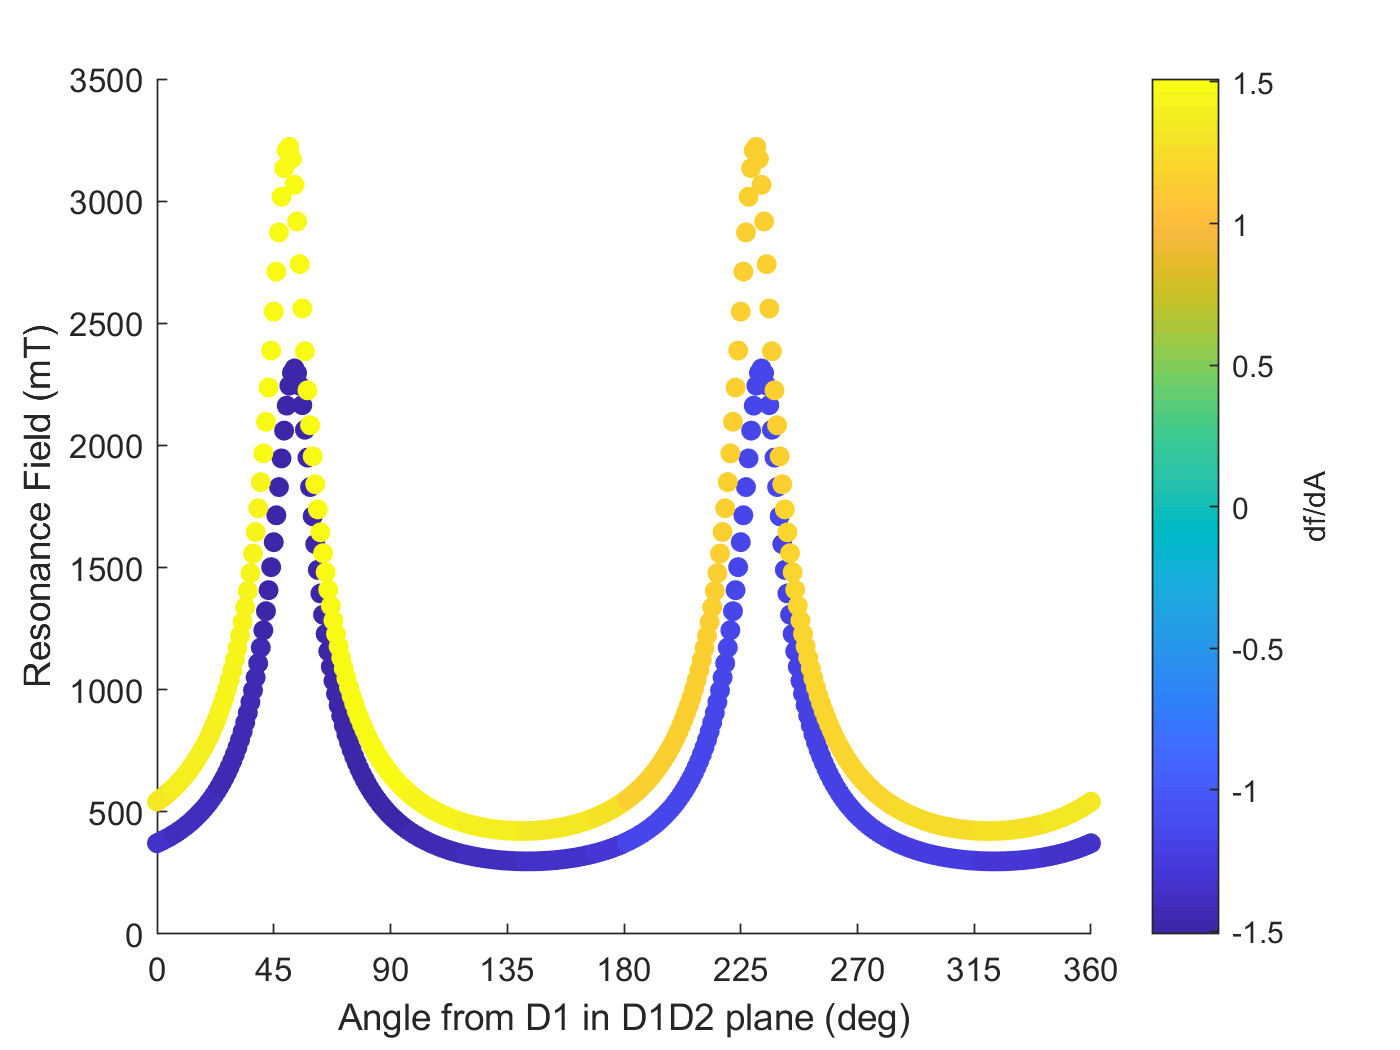
\includegraphics[width=\textwidth]{site2D1inD1D2planeA}
   \caption{\label{fig:site2D1inD1D2planeA}}
   \end{subfigure}
       \begin{subfigure}[b]{0.45\textwidth}
        \centering
        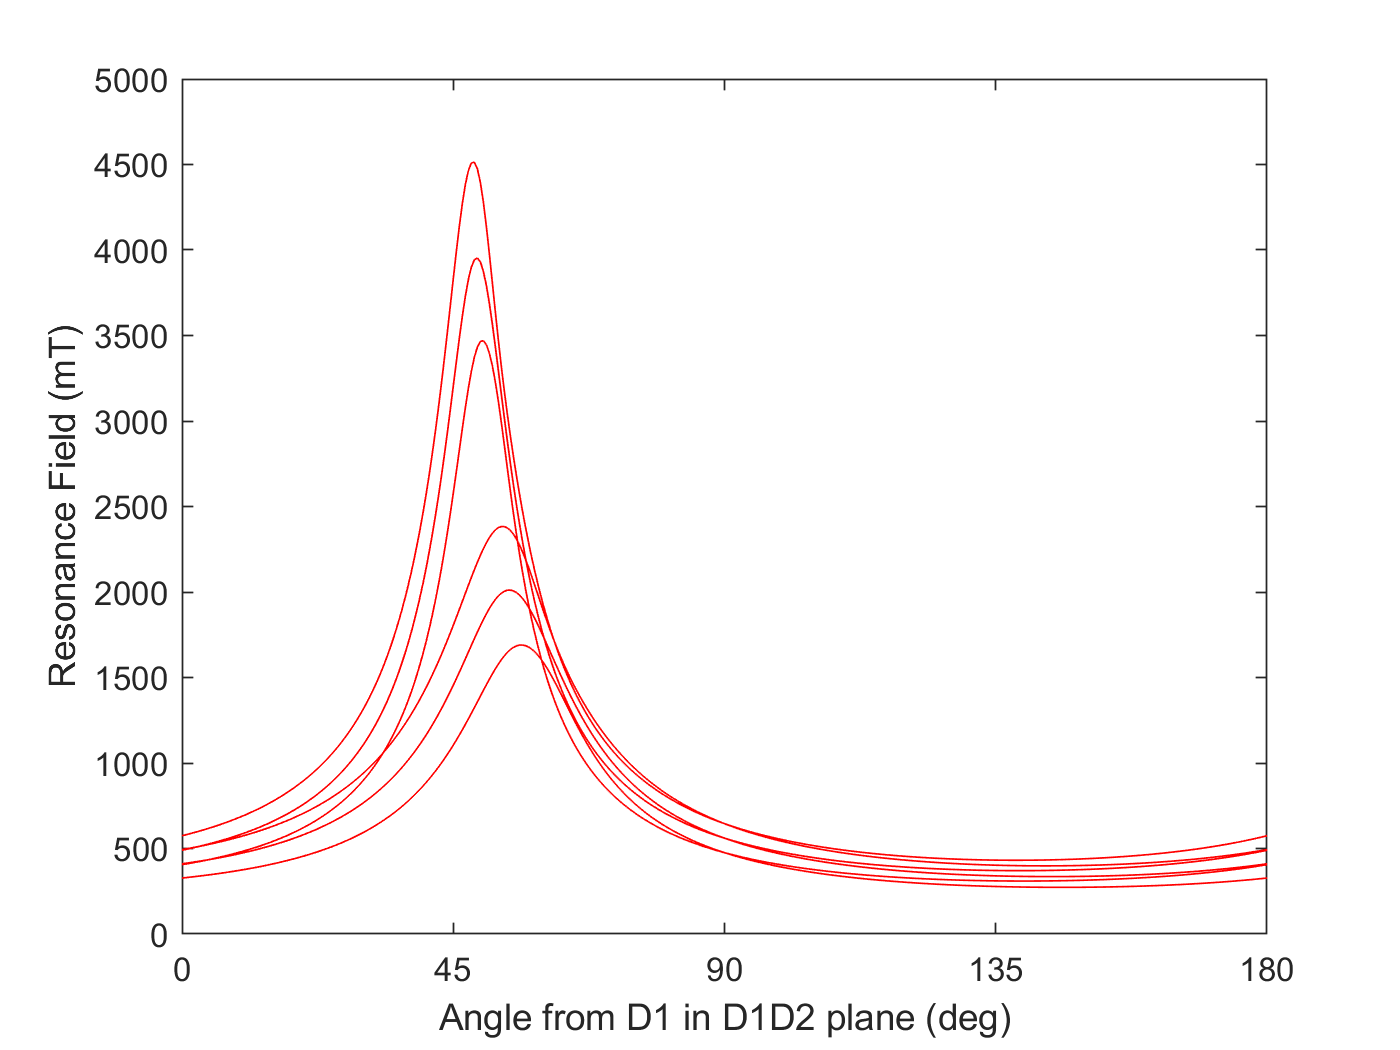
\includegraphics[width=\textwidth]{straininducedsplittingeasyspin}
   \caption{\label{fig:straininducedsplittingeasyspin}}
   \end{subfigure}
    \caption{Angular variations of the EPR transitions for site II $^{171}$Yb:YSO, where $\bm{B_{0}}$ is perpendicular the b-axis. The colour bar represents (a) $\Delta f/\Delta g$ for isotropic $\Delta g = 0.05$ and (b) $\Delta f/\Delta A$ for isotropic $\Delta A = 50$ MHz. (c) The 
    .}
\end{figure}

Therefore an alternative measurement approach was adopted. The magnetic field strength was swept over the region of the expected site II transitions for each additional mass stacked on top of the rotation plate. The transition detected for the initial $B_{0}$ sweep where the only applied strain is due to the weight of the sample rod in Fig.~\ref{fig:strainexpfirstfieldsweep} where six sharp peaks are detected. For due to the two-fold axis symmetry for this orientation the expectation is four site II EPR transitions. The additional measured peaks may be due to additional RE isotopes being present in the sample or weak amplitude forbidden $\Delta m_{I} = \pm 1$ transitions~\citep{PhysRevB.97.064409}. Comparison of experimental resonances to Fig~\ref{fig:straininducedsplittingeasyspin} where all site II transitions, including the forbidden transitions, are shown. Matching between the experimental and simulated EPR resonances determines the orientation in the $D1D2$ is $\theta = 120.5\pm 12.4^{\circ}$. If strain induces a dominant shift in the A-tensor then for the $m_{I}=0$ resonances the relative spacing between peaks is expected to change. However, if strain induces a shift in the g-tensor then the resonances are expected to shift in unison with an unaltered relative peak position. Fig.~\ref{fig:strainexpfirst1} presents shift in the EPR transitions as a function of the largest strain component is $\epsilon_{3}$ when unaxial stress ($\sigma_{3}$) is applied along the b-axis.     

\begin{figure}[H]
    \centering
    \begin{subfigure}[b]{0.45\textwidth}
        \centering
        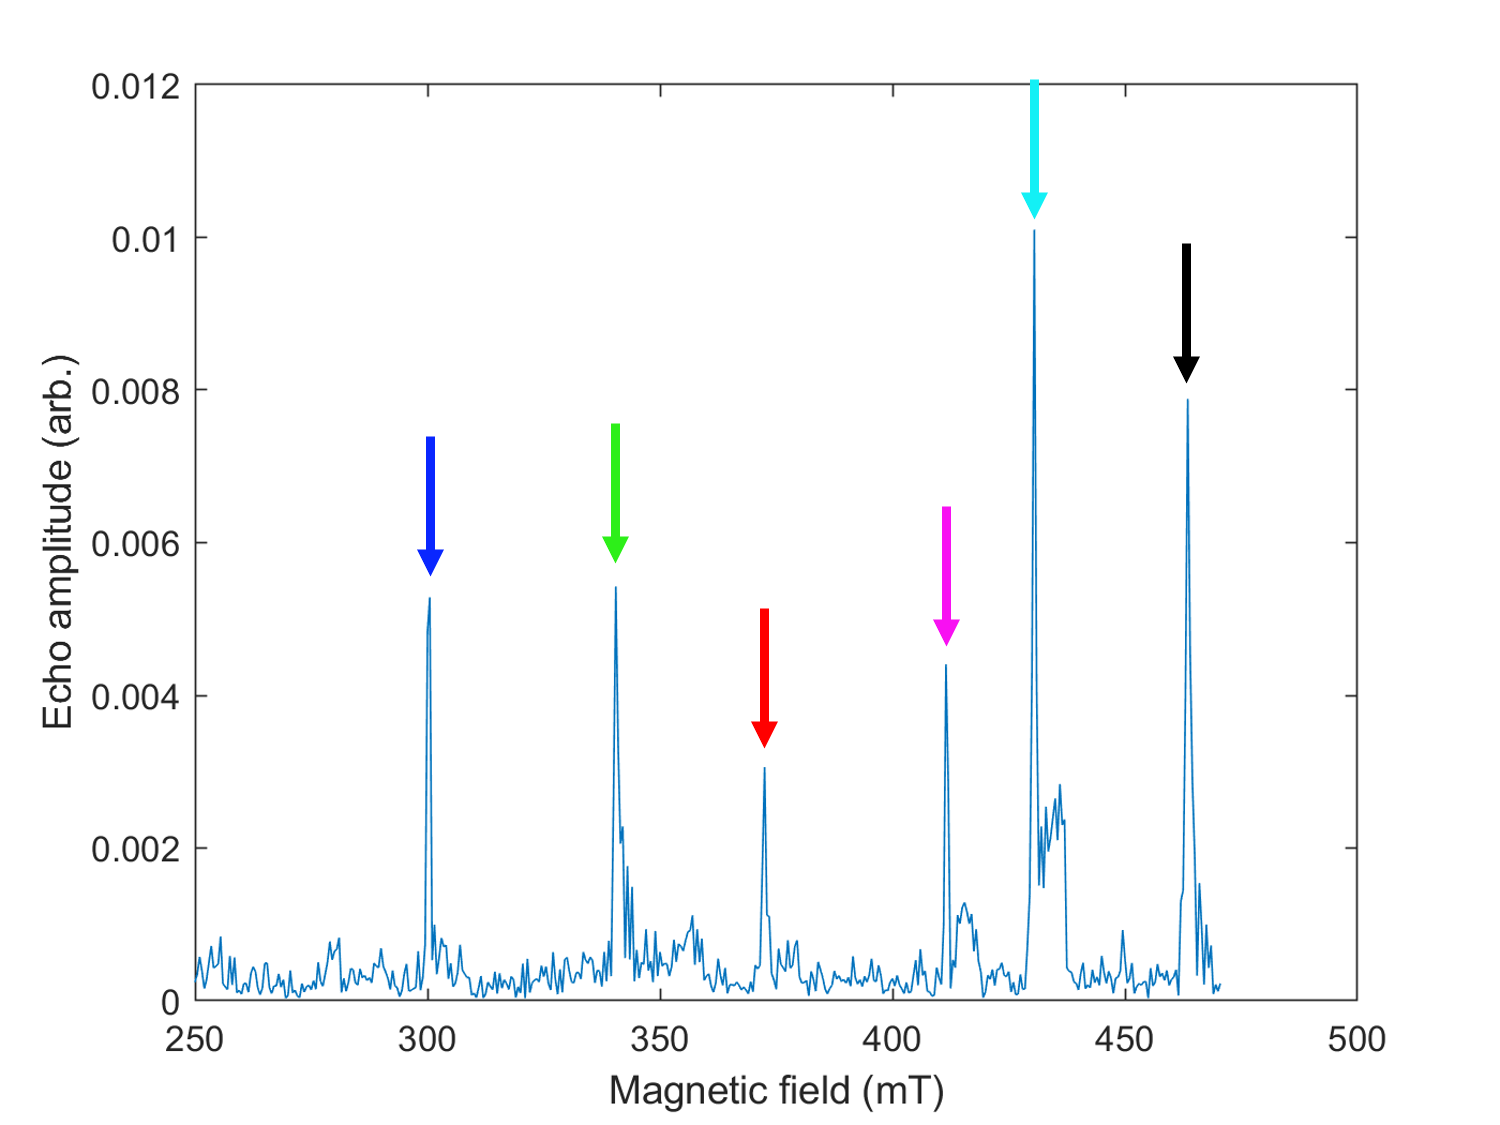
\includegraphics[width=\textwidth]{strainexpfirstfieldsweep}
        \caption{\label{fig:strainexpfirstfieldsweep}}
    \end{subfigure}
%     \hfill
    \begin{subfigure}[b]{0.45\textwidth}
        \centering
        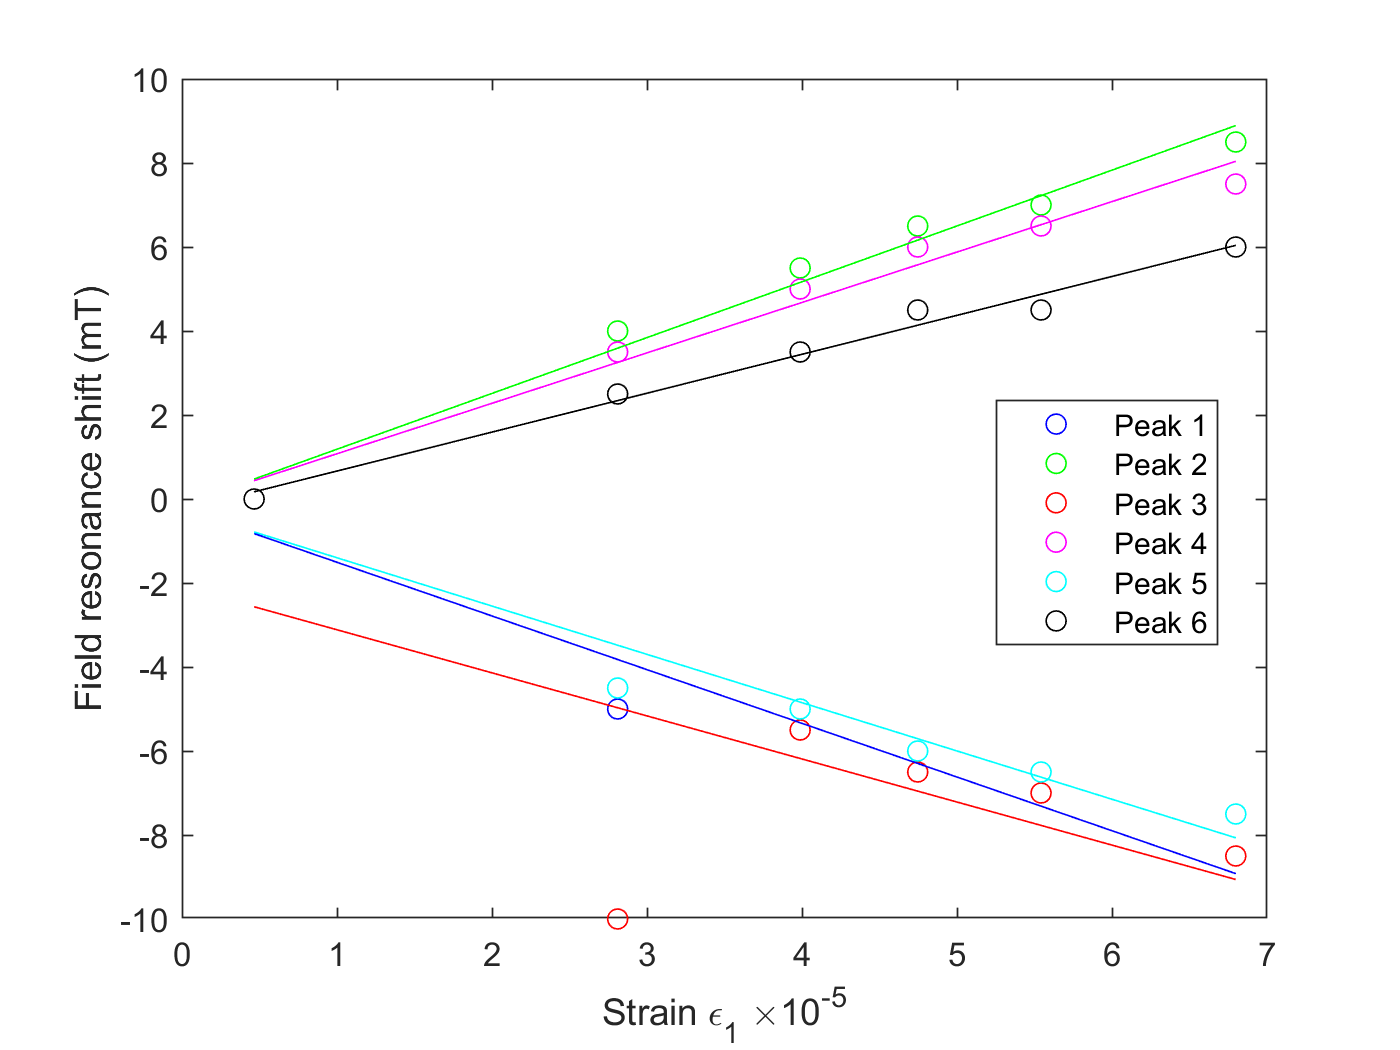
\includegraphics[width=\textwidth]{strainexpfirst1}
   \caption{\label{fig:strainexpfirst1}}
   \end{subfigure}
   \caption{(a) Magnetic field sweep over EPR transitions in site II with no mass on the rotation plate. (b) Magnetic resonance shift as a function of $\epsilon_{3}$ with applied linear fits. The sample orientation, $\theta$ = 120.5$\pm 12.4 ^{\circ}$ (or 300.5$\pm 12.4^{\circ}$) from $D1$ in the $D1D2$ plane.}
\end{figure}

Clipping of the echo signal was observed during the measurement of the data displayed in Fig.~\ref{fig:strainexpfirstfieldsweep}. Therefore, the function controlling the dynamic voltage range of the oscilloscope was modified such that the echo signal was no longer clipping. The experiment was repeater with finer sweeping around the resonances detected in the initial field sweep in Fig.~\ref{fig:strainexpsecondfieldsweep}. Lorentzian fitting of EPR resonances is completed as shown in Fig~\ref{fig:0gfittingpeaks} to obtain the peak amplitude, linewidth and resonance field values. Similarly the initial sample orientation is probed by comparing the EPR transitions in Fig.~\ref{fig:strainexpsecondfieldsweep} to Fig.~\ref{fig:straininducedsplittingeasyspin} although in this case a mass of 504 g is initially placed on the rotation plate. For the largest magnetic field resonance transition ($\ket{S=1/2,m_{I}=1/2} \leftrightarrow \ket{S=-1/2,m_{I}=1/2}$) shown by the black arrow in Fig.~\ref{fig:strainexpsecondfieldsweep} there is no site II orientation such that this EPR transition has a value below 430 mT. Therefore this could be an indicator that the strain has shifted the resonance. The ($\ket{S=1/2,m_{I}=-1/2} \leftrightarrow \ket{S=-1/2,m_{I}=-1/2}$) transition in green in Fig.~ref{fig:strainexpsecond1} appears to be insensitive to small changes of sample orientation such that orientation is $\theta =139.5 \pm 4^{\circ}$ (or 319.5$\pm 4^{\circ}$).          

\begin{figure}[H]
    \centering
    \begin{subfigure}[b]{0.45\textwidth}
        \centering
        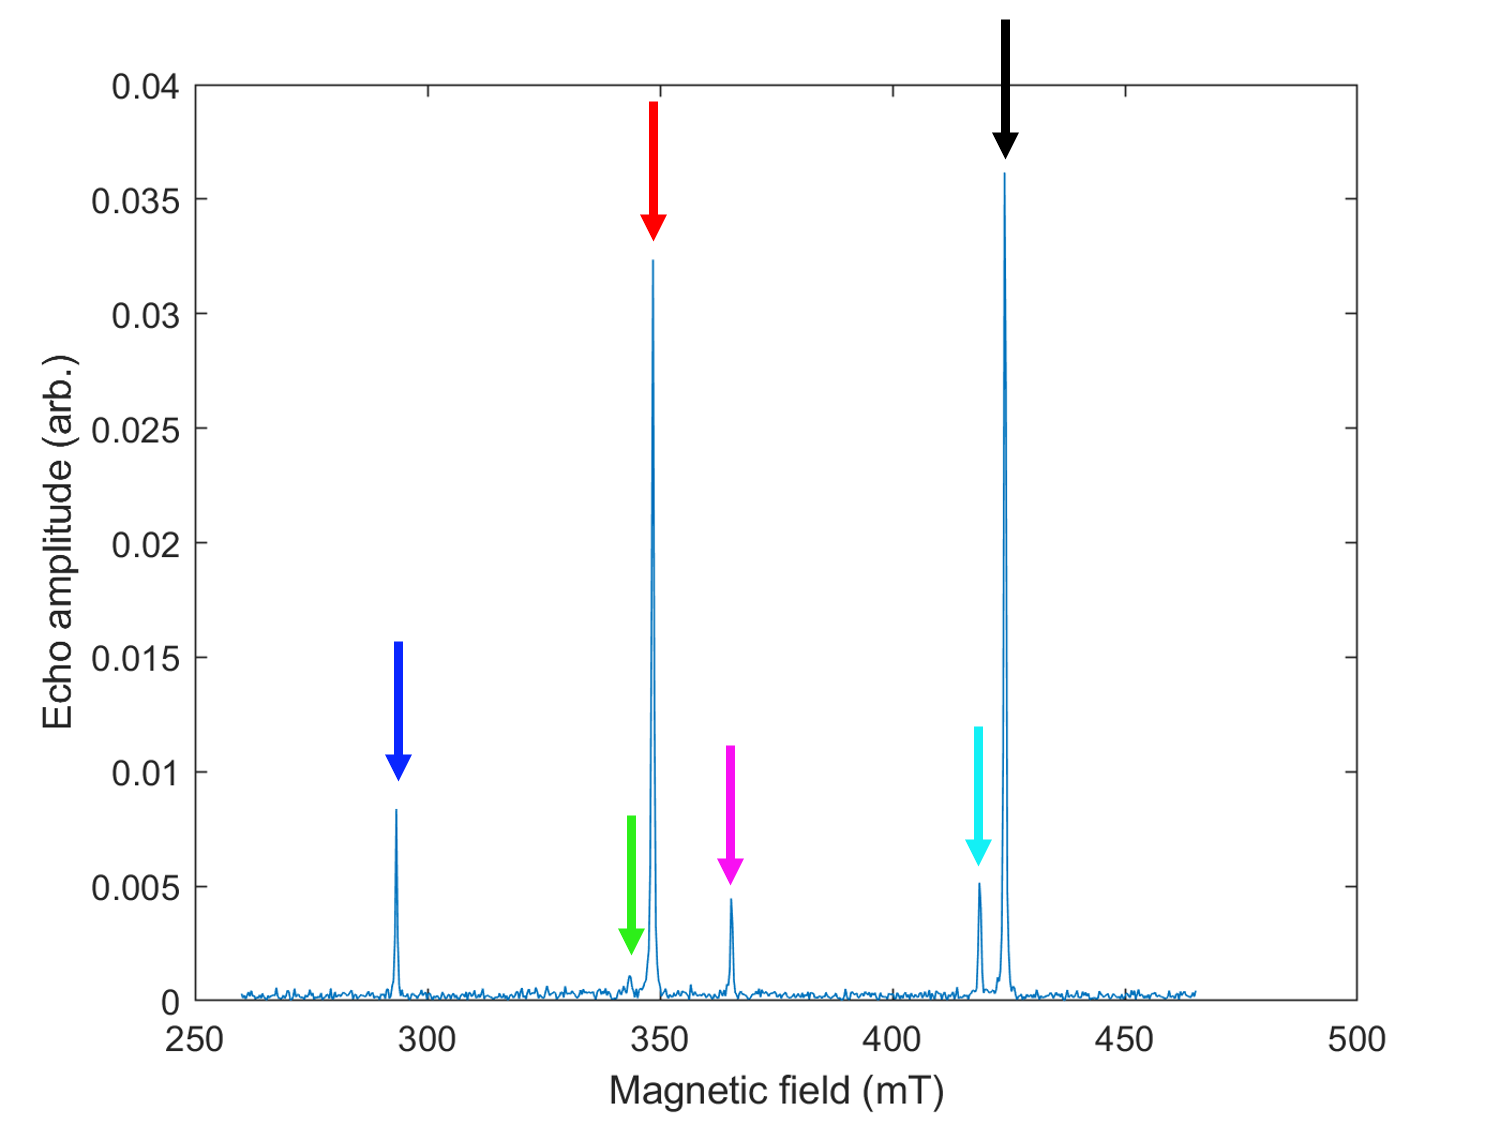
\includegraphics[width=\textwidth]{strainexpsecondfieldsweep}
        \caption{\label{fig:strainexpsecondfieldsweep}}
    \end{subfigure}
%     \hfill
    \begin{subfigure}[b]{0.45\textwidth}
        \centering
        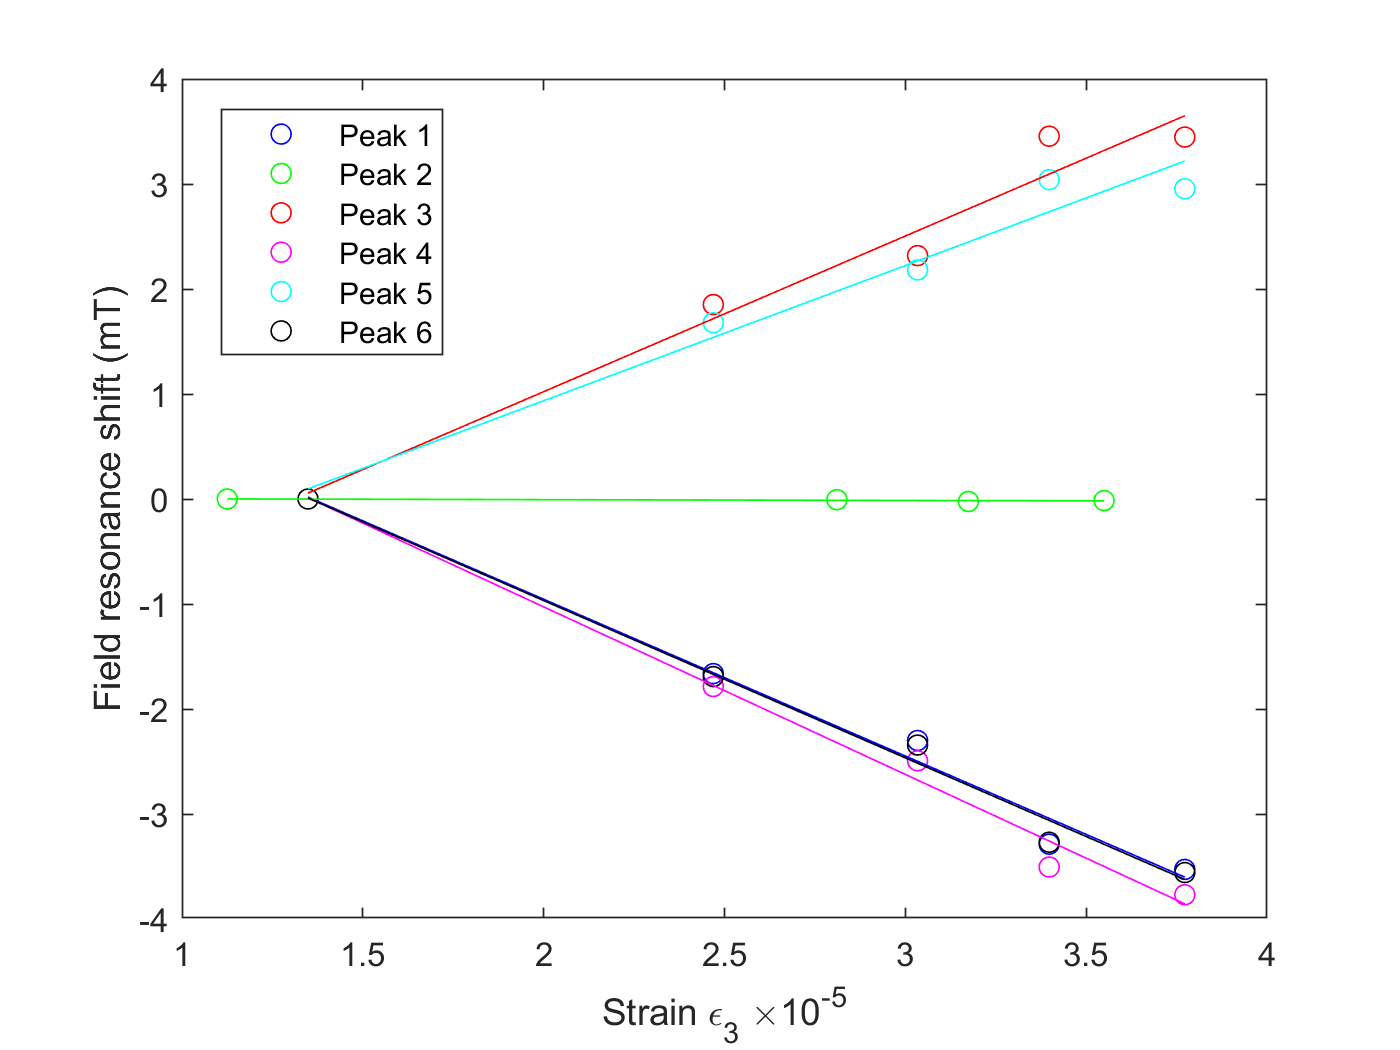
\includegraphics[width=\textwidth]{strainexpsecond1}
   \caption{\label{fig:strainexpsecond1}}
   \end{subfigure}
       \begin{subfigure}[b]{0.45\textwidth}
        \centering
        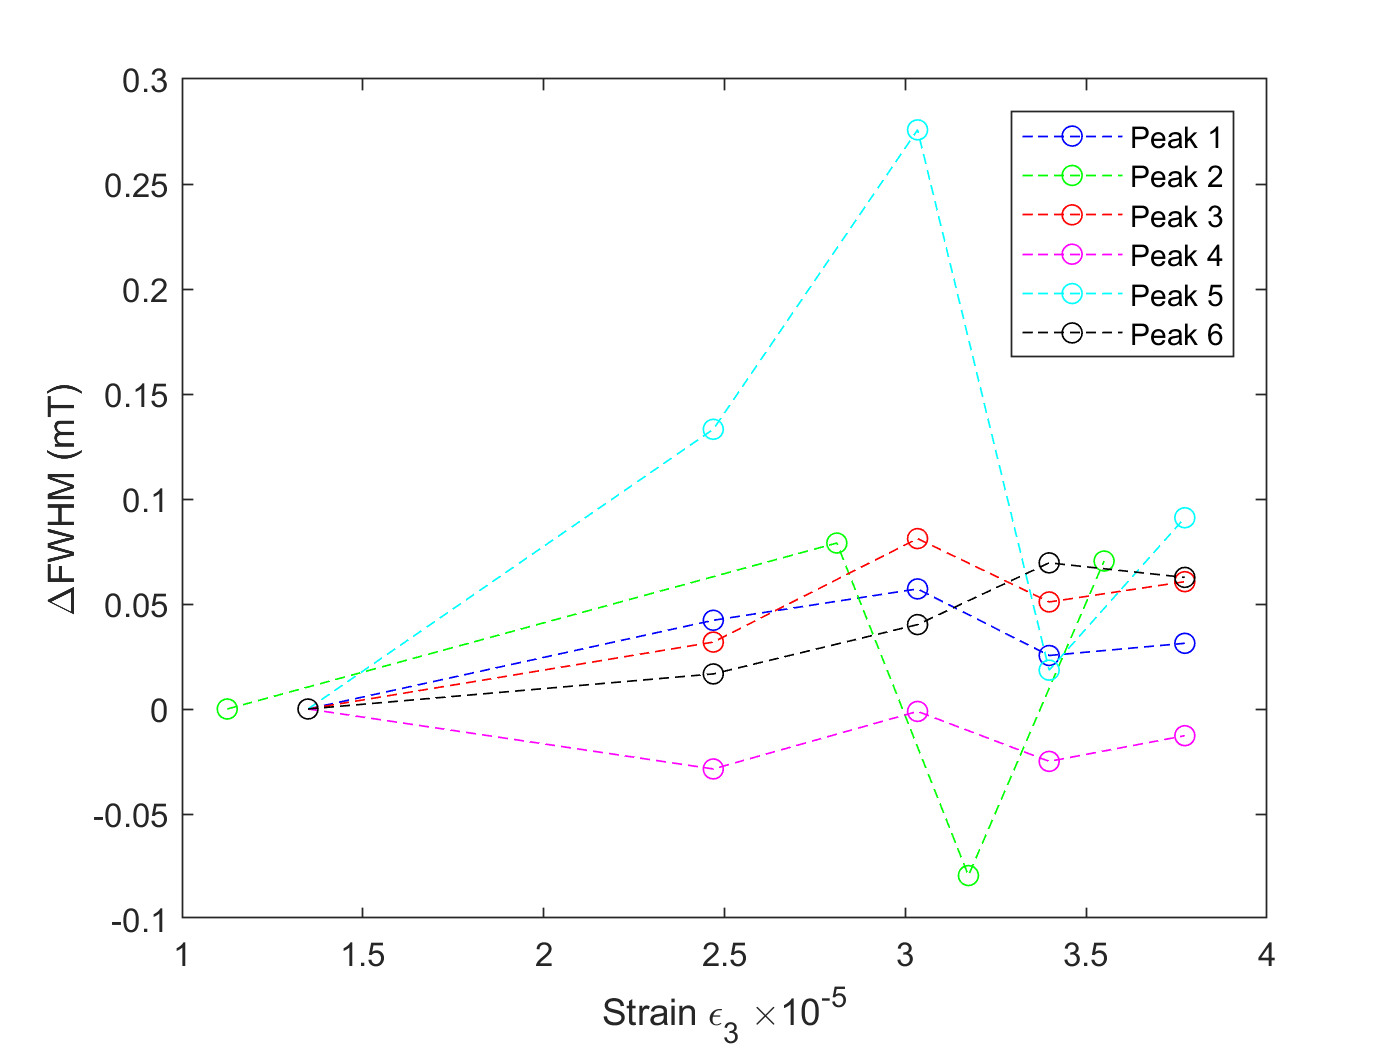
\includegraphics[width=\textwidth]{strainexpsecond2}
   \caption{\label{fig:strainexpsecond1}}
   \end{subfigure}
       \begin{subfigure}[b]{0.45\textwidth}
        \centering
        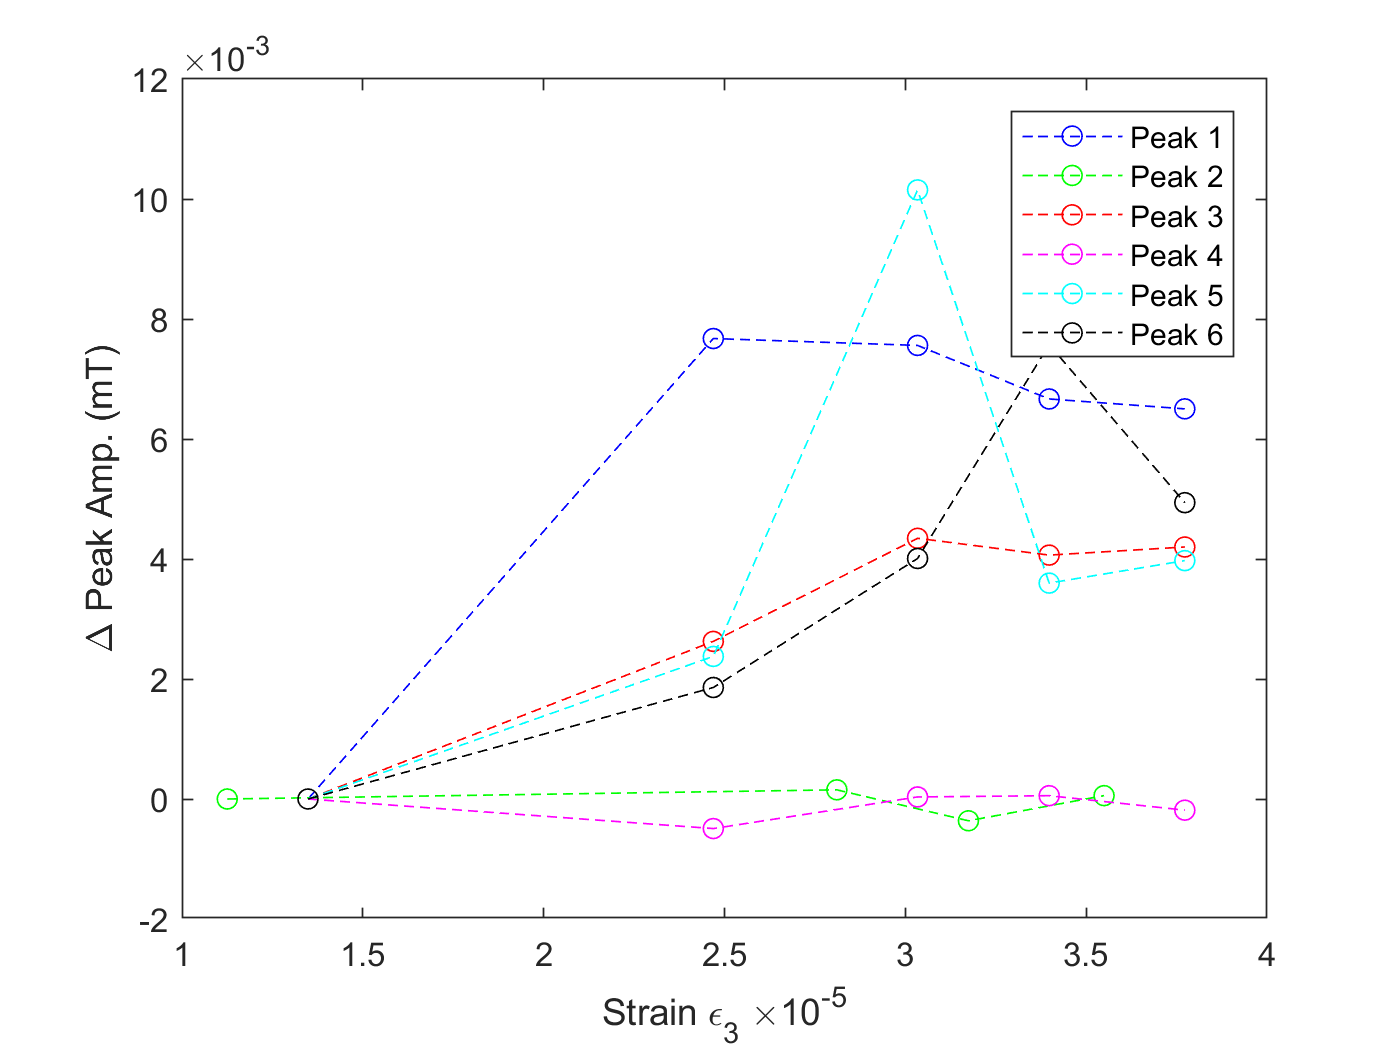
\includegraphics[width=\textwidth]{strainexpsecond3}
   \caption{\label{fig:strainexpsecond1}}
   \end{subfigure}
   \caption{Yb:YSO site II EPR transitions for $\theta$ = 139.5$\pm 4^{\circ}$ (or 319.5$\pm 4^{\circ}$) from $D1$ in the $D1D2$ plane. (a) Magnetic field sweep over EPR transitions with 504 g mass initially on the rotation plate. (b) Magnetic resonance shift as a function of $\epsilon_{3}$ with applied linear fits. (c) Change in the EPR linewidth (full width half maximum FWHM) vs. $\epsilon_{3}$. (d) Change in the resonance signal amplitude vs. $\epsilon_{3}$.}
\end{figure}

Next the sample was rotated by 180$^{\circ}$ since for a small perturbation of $\bm{A}$ on sample orientation with respect to the $B_{0}$ generates a larger value of $df/dA$. The magnetic field sweep in Fig.~\ref{fig:strainexpthirdfieldsweep} revealed an additional weak echo signal. As expected the apparent insensitivity of the red transition peak of Fig.~\ref{fig:strainexpthird1} is used to determine sample orientation of $\theta=$319.5$\pm 4^{\circ}$ (or $139.5 \pm 4^{\circ}$). Measured approximately linear shift of the resonance field as $\epsilon_{3}$ is increased is shown in Fig.~\ref{fig:strainexpthird1} where the additionally cross markers display the measurements as the masses are removed from the rotation plate. The all resonances shift significantly, excluding peak 3, as the masses are removed which is expected to be the product of unwanted sample rotation. 

\begin{figure}[H]
    \centering
    \begin{subfigure}[b]{0.45\textwidth}
        \centering
        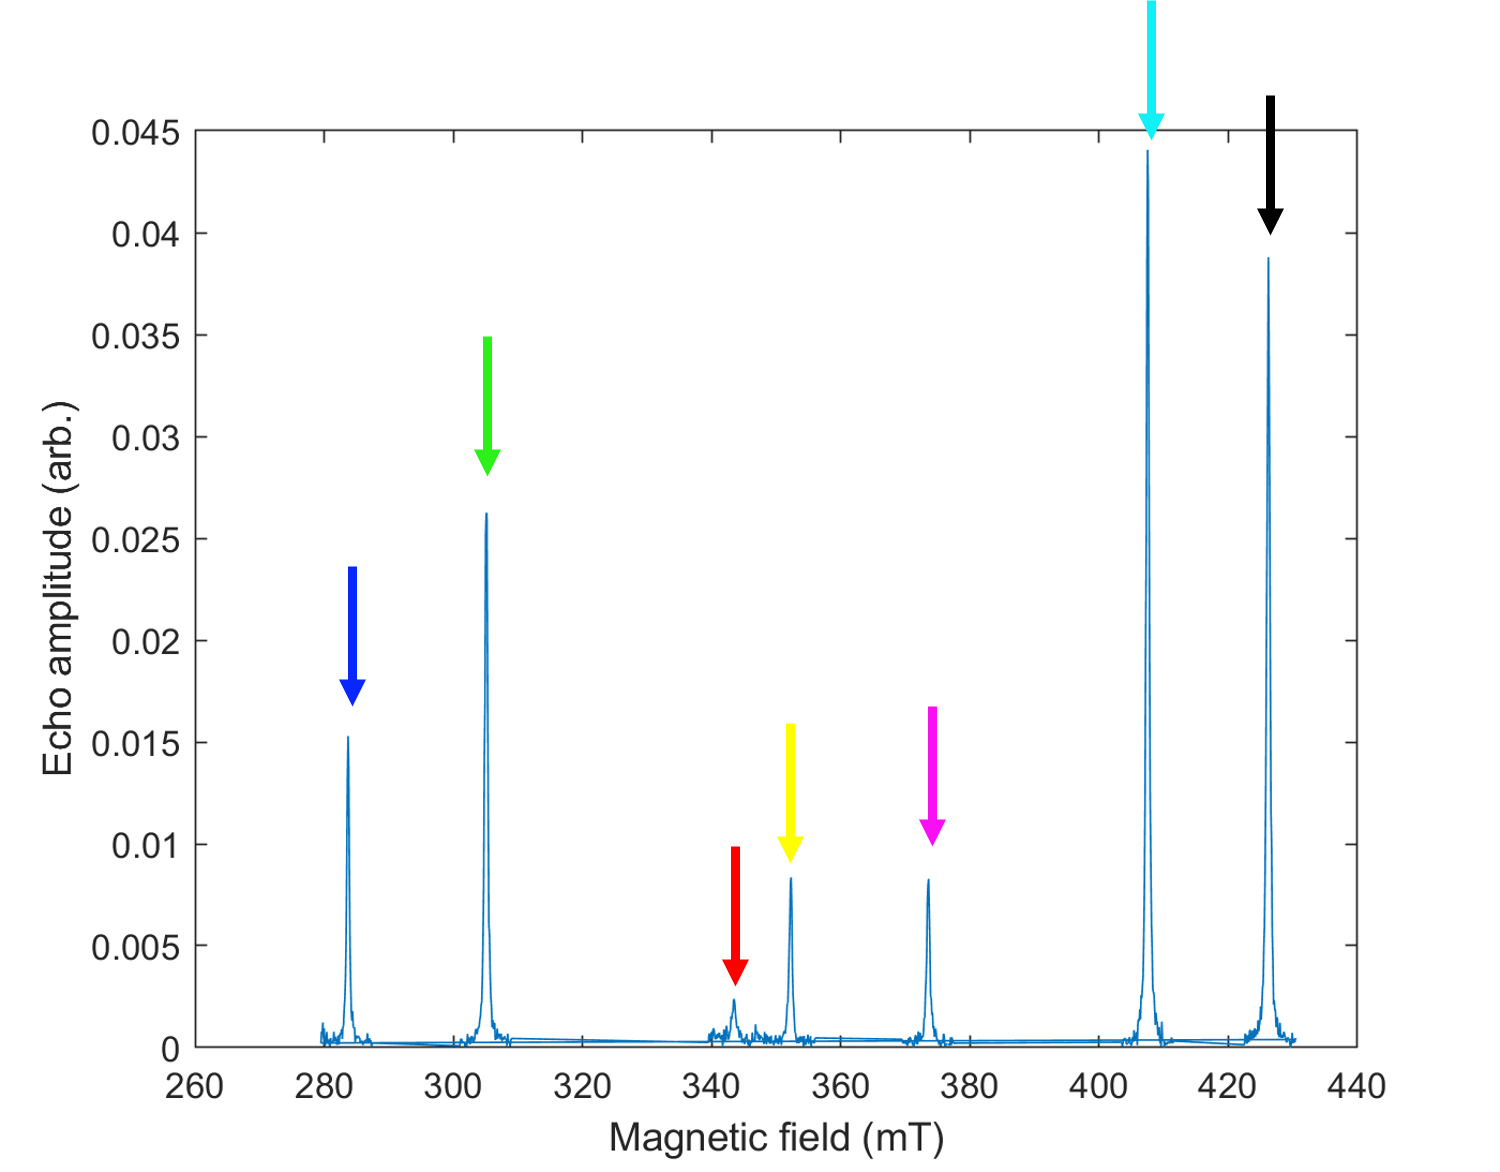
\includegraphics[width=\textwidth]{strainexpthirdfieldsweep}
        \caption{\label{fig:strainexpthirdfieldsweep}}
    \end{subfigure}
%     \hfill
    \begin{subfigure}[b]{0.45\textwidth}
        \centering
        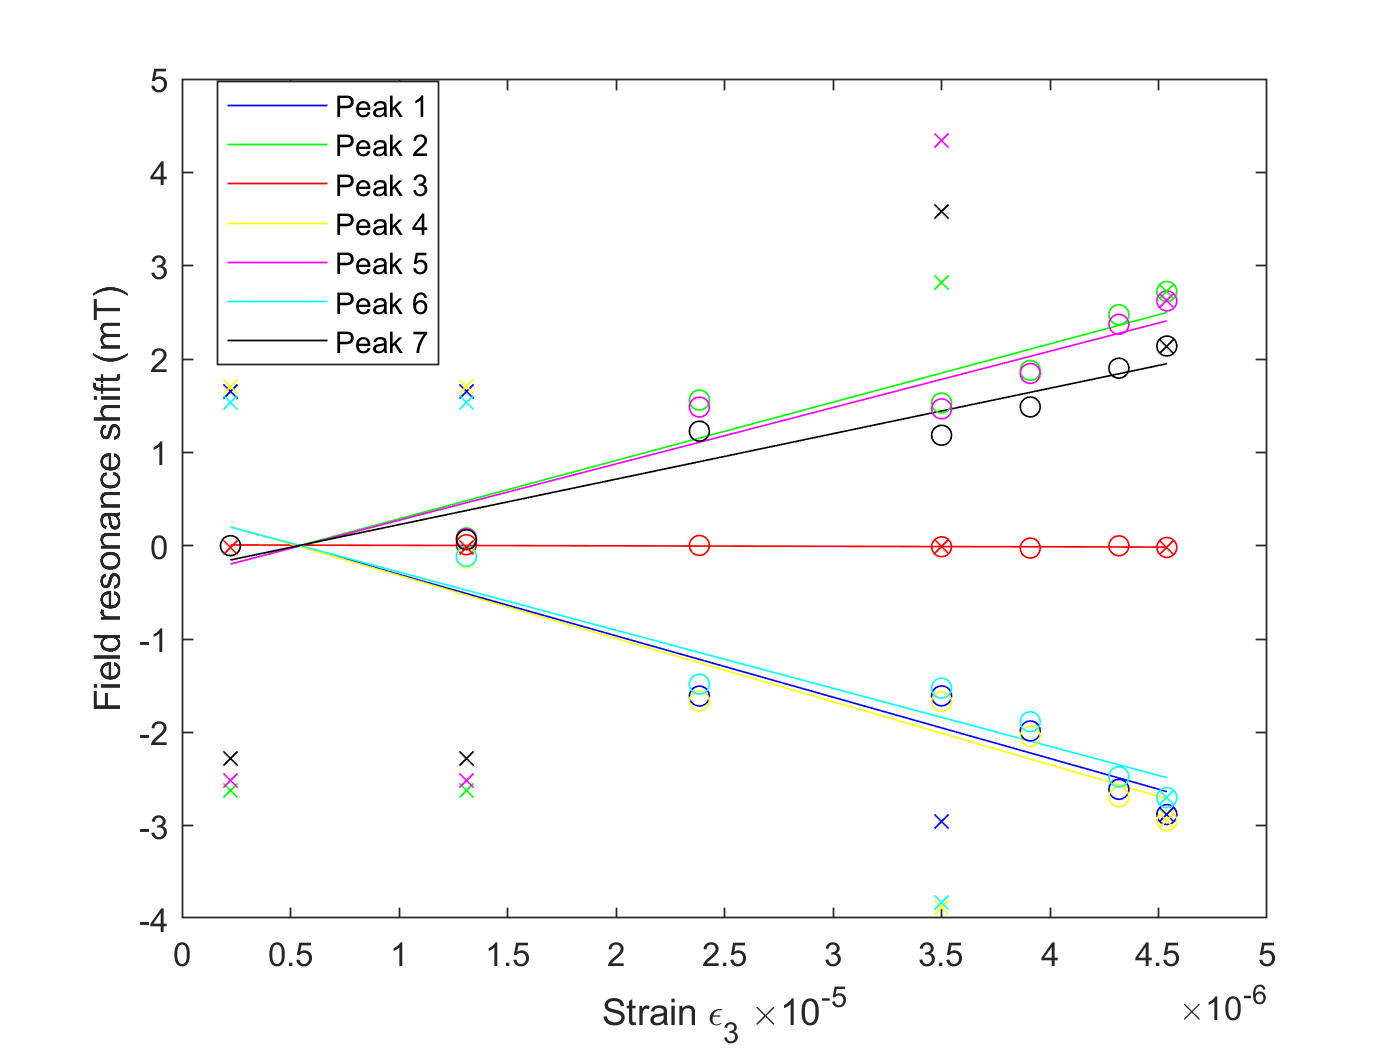
\includegraphics[width=\textwidth]{strainexpthird1}
   \caption{\label{fig:strainexpthird1}}
   \end{subfigure}
   \caption{Yb:YSO site II EPR transitions for $\theta$ = 139.5$\pm 2^{\circ}$ (or 319.5$\pm 2^{\circ}$) from $D1$ in the $D1D2$ plane. (a) Magnetic field sweep over EPR transitions with 504 g mass initially on the rotation plate. (b) Magnetic resonance shift as a function of $\epsilon_{3}$ with applied linear fits.}
\end{figure}










    \chapter{Outlook}

\section{\label{sec:discussion}Discussion}
Gaining insight into the effect strain induced in crystal and has on the $g$ and $A$ is not a trivial question. In particular the highly anisotropic nature of $YSO$ makes separating the sensitivity to changes in the orientation of $B_{0}$ with respect to the dielectric axis and strain mechanism difficult. For this experimental setup where the sample is hosted in a customised sample holder was designed to allow rotation of the crystal such that experiments could be completed for a variety or orientations. However, the free rotation of the sample hindered the ability to investigate a particular orientation whilst stacking mass on top of the rotation plate. 

Therefore, either the sample rod could be clamped tightly in place to the probe meaning the mass placed on the rotation plate would have no impact on the stress applied to the sample or the connection is loosen and suspected dominant mechanism observed from the sample rotation. It appears in Fig.~\ref{fig:strainexpsecond1} and Fig.~\ref{fig:strainexpthird1} this may be the case as the $\ket{S=1/2,m_{I}=-1/2} \leftrightarrow \ket{S=-1/2,m_{I}=-1/2}$ transition for those angular rotations appears to be fairly insensitivity to crystal rotation with not notable magnetic field resonance shift. Yet the transition shown to be sensitive to small angular rotations in Fig.~\ref{fig:straininducedsplittingeasyspin} undergoes approximately linear shifts. Similarly, measurements of the resonance linewidth in particular for Fig.~\ref{fig:strainexpthird2} appears to show an upwards trend which suggests strain could be the mechanism similarly as it is in Ref.~\citep{PhysRevLett.115.057601}.

Interestingly upon comparison to the simulated EPR spectrum as a function of angular rotation to the experimentally measured EPR peaks in for example Fig.~\ref{fig:strainexpfirstfieldsweep} can be related with good agreement for the $\theta$ = 120.5$\pm 12.4 ^{\circ}$ crystal orientation. Thus each transition undergoes the opposite sign shift to their magnetically degenerate counterpart. The observation is made that the dipole allowed transitions are not shifting in opposite directions as result of the stress applied to the crystal which indicates the strain is producing a reduction in the hyperfine coupling strength.


\section{Conclusions and Future Work}
Despite the experimental results of the investigation of induced shifts of the $g$ and $A$-tensor currently being inconclusive due to the crystal sample rotation during measurement, this research could help to inform future experimental schemes involving YSO. The ability to rotate the sample to different orientations whilst the sample is in the cryostat is beneficial. However, investigation of using a fixed probe would be interesting and where such a setup is not necessarily be trivial to fabricate. The issue is trying to manage the need to secure the sample so that it cannot move but also enable the application of mechanical stress to the sample surface. An alternative optical may be to apply strain using a piezo-actuator such as in \citep{PhysRevLett.115.057601}. Additionally the crystal orientation chosen was dictated by the region where rate of change of the magnetic field resonances as a function of $\theta$ was lowest. However, the broader site I transitions provide larger values of $df/dg$ and would be interesting to investigate next.  

Conversely, the emphasis during measurement on trying to eliminate any crystal rotation may have hindered the ability to effectively measure effects due to applied strain. The clamp connecting the sample holder to the EPR probe may have been preventing the full force due to the masses being applied to the crystal. Additionally, certain transitions were observed to be less sensitive to angular rotations. Therefore, loosening to the friction between the rod and the focusing on the $\ket{S=1/2,m_{I}=-1/2} \leftrightarrow \ket{S=-1/2,m_{I}=-1/2}$ transition may reveal shift resulting from the stress mechanism. Additionally, an initial attempt was made to characterise the effect of small crystal rotations to decouple the transitions from this effect by rotating the crystal in 5-10 $^{\circ}$ increments. However, the sample sensitivity to rotations and the number of transitions in this sample results in many crossings between transitions making it time-consuming and difficult to track for these rotational increments.  

Lastly, another avenue for future exploration is the density function theory calculations used to calculate the stiffness coefficients in Ref.~\citep{Ceramics}. The treatment of the Spin Hamiltonian terms in this model may aid the ability to determined the unknown coefficients of the $\bm{\mathcal{G}}$ and $\bm{\mathcal{A}}$ tensors. 




    
    \renewcommand\bibname{References} % Change Bibliography name to References
\printbibliography 
\appendix

	\appendixpage
    \noappendicestocpagenum
    \addappheadtotoc

	%\input{89.Related_Work}
    \chapter{YSO}

\begin{table}[h]
  \begin{center}
    \caption{Y$_{2}$SiO$_{5}$ theoretical second-order elastic coefficients (GPa)}
    \label{tab:elasticcoefficients}
    \begin{tabular}{l|r r r r r r r r r r r r r r} 
    \hline % <-- Changed to S here.
Space group & $c_{11}$ & $c_{22}$ & $c_{33}$ & $c_{44}$ & $c_{55}$ & $c_{66}$ & $c_{12}$ & $c_{13}$ & $c_{15}$ & $c_{23}$ & $c_{25}$ & $c_{35}$ & $c_{46}$ \\
       \hline
$B2/b$~\citep{doi:10.1111/jace.12764} & 226 & 201 & 156 & 44 & 67 & 63 & 88 & 59 & 5 & 27 & -0.3 & -0.2 & 10 \\ 
$C2/c$~\citep{Ceramics} & 226 & 156 & 201 & 44 & 63 & 67 & 59 & 88 & 5 & 27 & -0.3 & -0.2 & 10 \\
\hline
    \end{tabular}
  \end{center}
\end{table}

\begin{table}[h]
  \begin{center}
    \caption{Y$_{2}$SiO$_{5}$ theoretical second-order elastic coefficients}
    \label{tab:elasticcoefficients}
    \begin{tabular}{l|r r r r r r r r r r r r r r} 
    \hline % <-- Changed to S here.
Space group & $c_{11}$ & $c_{22}$ & $c_{33}$ & $c_{44}$ & $c_{55}$ & $c_{66}$ & $c_{12}$ & $c_{13}$ & $c_{15}$ & $c_{23}$ & $c_{25}$ & $c_{35}$ & $c_{46}$ \\
       \hline
$C2/c$ & 226 & 156 & 201 & 44 & 63 & 67 & 59 & 88 & 5 & 27 & -0.3 & -0.2 & 10 \\
\hline
    \end{tabular}
  \end{center}
\end{table}





\begin{figure}[H]
    \centering
    \begin{subfigure}[b]{0.487\textwidth}
        \centering
        \includegraphics[width=\textwidth]{C2c}
        \caption{$C2/c$}
    \end{subfigure}
%     \hfill
    \begin{subfigure}[b]{0.4\textwidth}
        \centering
        \includegraphics[width=\textwidth]{I2a}
   \caption{$I2/a$}
   \end{subfigure}
    \caption{Comparison of the Y$_{2}$SiO$_{5}$ unit cell for the (a) $C2/c$ and (b) $I2/a$ space group obtained from the inorganic crystal structure database (collection code: 291362).}
\label{fig:crystalspacegroups}
\end{figure}

\begin{table}[h]
 \begin{center}
  \caption{Y$_{2}$SiO$_{5}$ $I2/a$ lattice parameters\citep{doi:10.1021/acsami.5b00445}.}
  \label{tab:I2alatticeparam}
  \begin{tabular}{l | c}
  \hline
  Lattice constants & Theoretical\\
  \hline
  a ($\AA$) &  10.40\\
  b ($\AA$) &  6.71\\
  c ($\AA$) &  12.47\\
  $\beta$ ($^{\circ}$) &  102.6\\
  \hline
    \end{tabular}
  \end{center}
\end{table}

\begin{figure}[h]
\centering
\includegraphics[height=0.32\textwidth,keepaspectratio]{D1bD2abc}
\caption{\label{fig:D1bD2abc} Orientation of YSO $C2/c$ crystallographic axis with respect to the optical axis \citep{SHOUDU1999901}.}
\end{figure}





    \chapter{\label{sec:sampleprobefabrication}Sample probe fabrication}

\begin{figure}[h]
\centering
\includegraphics[height=0.32\textwidth,keepaspectratio]{cryostatimage}
\caption{\label{fig:experimentalsetup} Image of components of the EPR experimental set up.}
\end{figure}


\begin{figure}[H]
    \centering
    \begin{subfigure}[b]{0.4\textwidth}
        \centering
        \includegraphics[width=\textwidth]{CNC3}
        \caption{}
    \end{subfigure}
%     \hfill
    \begin{subfigure}[b]{0.4\textwidth}
        \centering
        \includegraphics[width=\textwidth]{CNC1}
   \caption{}
   \end{subfigure}
       \begin{subfigure}[b]{0.4\textwidth}
        \centering
        \includegraphics[width=\textwidth]{CNC2}
   \caption{}
   \end{subfigure}
   \caption{Images of the Computer numerical control (CNC) machine used to fabricate the acrylic sample holder pieces. (a) iModel creator software used to define the design. (b) CNC machine containing a drill piece which is used to mill the sample material. (c) Milling of cylindrical acrylic pieces.}
\end{figure}


\begin{figure}[H]
    \centering
    \begin{subfigure}[b]{0.35\textwidth}
        \centering
        \includegraphics[width=\textwidth]{acrylicpieces}
        \caption{}
    \end{subfigure}
%     \hfill
    \begin{subfigure}[b]{0.3\textwidth}
        \centering
        \includegraphics[width=\textwidth]{adapterrods}
   \caption{}
   \end{subfigure}
       \begin{subfigure}[b]{0.2\textwidth}
        \centering
        \includegraphics[width=\textwidth]{fullprobesetup}
   \caption{}
   \end{subfigure}
   \caption{Image of (a) the acrylic sample holders, (b) the adapter rods and (c) resonator probe (left) and rod pieces (right).}
\end{figure}


\begin{figure}[H]
    \centering
    \begin{subfigure}[b]{0.3\textwidth}
        \centering
        \includegraphics[width=\textwidth]{ybysosample}
        \caption{}
    \end{subfigure}
%     \hfill
    \begin{subfigure}[b]{0.3\textwidth}
        \centering
        \includegraphics[width=\textwidth]{sampleloading}
   \caption{}
   \end{subfigure}
       \begin{subfigure}[b]{0.3\textwidth}
        \centering
        \includegraphics[width=\textwidth]{sampleloading2}
   \caption{}
   \end{subfigure}
   \caption{The transparent $^{171}$Yb$^{3+}$:YSO sample and circular acrylic piece used to separate the base piece from the sample when sample is inside the sample holder. (b) The cryogenic tape connecting the adapter to the base piece. (c) String connecting the base plate to the probe is used as a fail-safe.}
\end{figure}
    \chapter{\label{sec:easyspinsim}EasySpin simulations}

\begin{figure}[H]
    \centering
    \begin{subfigure}[b]{0.3\textwidth}
        \centering
        \includegraphics[width=\textwidth]{NdflaigrespectD1}
        \caption{Rotation (360 $^{\circ}$)
around crystal b axis ($\phi$ = 69.83 $^{\circ}$, $\theta$
= 3.75 $^{\circ}$)}
    \end{subfigure}
%     \hfill
    \begin{subfigure}[b]{0.3\textwidth}
        \centering
        \includegraphics[width=\textwidth]{NdflaigrespectD2}
   \caption{Rotation (180 $^{\circ}$)
around crystal D1 axis
($\phi$ = 189.13 $^{\circ}$, $\theta$= 96.21 $^{\circ}$)}
   \end{subfigure}
      \begin{subfigure}[b]{0.3\textwidth}
        \centering
        \includegraphics[width=\textwidth]{NdflaigrespectD12}
   \caption{Rotation (180 $^{\circ}$)
around crystal D2 axis
($\phi$ = 89.72 $^{\circ}$, $\theta$
= 92.77 $^{\circ}$)}
   \end{subfigure}
   \caption{Angular variation of the hyperfine resonance fields of both sub sites (green and
black) for $145$Nd$^{3+}$ doped YSO. Experimental values (cross) and fit (line). Copy from Ref.\citep{mairflaig}.}
   \label{fig:mairflaigthesis}
    \end{figure}
    
    \begin{figure}[H]
    \centering
    \begin{subfigure}[b]{0.45\textwidth}
        \centering
        \includegraphics[width=\textwidth]{crystalbaxis}
        \caption{Rotation (360 $^{\circ}$)
around crystal b axis ($\phi$ = 69.83 $^{\circ}$, $\theta$
= 3.75 $^{\circ}$)}
    \end{subfigure}
%     \hfill
    \begin{subfigure}[b]{0.45\textwidth}
        \centering
        \includegraphics[width=\textwidth]{crystalD1axis1}
   \caption{Rotation (360 $^{\circ}$)
around crystal D2 axis
($\phi$ = 89.72 $^{\circ}$, $\theta$
= 92.77 $^{\circ}$)}
   \end{subfigure}
      \begin{subfigure}[b]{0.45\textwidth}
        \centering
        \includegraphics[width=\textwidth]{crystalD2axis}
   \caption{Rotation (360 $^{\circ}$)
around crystal D2 axis
($\phi$ = 89.72 $^{\circ}$, $\theta$
= 92.77 $^{\circ}$)}
   \end{subfigure}
   \caption{Simulation of the angular variation of the hyperfine resonance fields of both sub sites (green and
black) for $145$Nd$^{3+}$ doped YSO.}
   \label{fig:mairflaigthesisreplicate}
    \end{figure}



    \chapter{\label{sec:additionalresults}Additional Results}

\begin{figure}[h]
\centering
\includegraphics[height=0.5\textwidth,keepaspectratio]{T1naturalSi}
\caption{\label{fig:T1naturalSi} Inversion recovery pulse sequence of natural Si doped with P to determine $T_{1} \approx 20$ ms. The in-phase (I) and out-of-phase (Q) signals are shown in blue and red, respectively.}
\end{figure}

\begin{figure}[H]
    \centering
    \begin{subfigure}[b]{0.45\textwidth}
        \centering
        \includegraphics[width=\textwidth]{YbYSORabi}
        \caption{\label{fig:YbYSORabi}}
    \end{subfigure}
%     \hfill
    \begin{subfigure}[b]{0.45\textwidth}
        \centering
        \includegraphics[width=\textwidth]{YbYSOT1}
   \caption{\label{fig:YbYSOT1}}
   \end{subfigure}
   \begin{subfigure}[b]{0.45\textwidth}
        \centering
        \includegraphics[width=\textwidth]{YbYSOT2}
        \caption{\label{fig:YbYSOT2}}
    \end{subfigure}
    \caption{$^{171}$Yb$^{3+}$:YSO site II (a) Rabi oscillations, (b) $T_{1}$ relaxation curve where $T_{1}\approx 2.6$ ms and (c) $T_{2}$ relaxation curve where $T_{2} \approx 9$ $\mu$s. The in-phase (I) and out-of-phase (Q) signals are shown in blue and red, respectively.}
\end{figure}


\begin{figure}[h]
\centering
\includegraphics[height=0.5\textwidth,keepaspectratio]{cleanecho}
\caption{\label{fig:cleanecho} $^{171}$Yb$^{3+}$:YSO site II single-shot echo detection. The in-phase (I) and out-of-phase (Q) signals are shown in blue and red, respectively.}
\end{figure}


\begin{figure}[h]
\centering
\includegraphics[height=0.5\textwidth,keepaspectratio]{0gfittingpeaks}
\caption{\label{fig:0gfittingpeaks} $^{171}$Yb$^{3+}$:YSO resonance peak for a site II transition as the unaxial stress is increased. The b-axis is perpendicular to $B_{0}$ where $\theta$ = 120.5$\pm 12.4 ^{\circ}$ (or 300.5$\pm 12.4^{\circ}$).}
\end{figure}

\begin{figure}[H]
    \centering
    \begin{subfigure}[b]{0.45\textwidth}
        \centering
        \includegraphics[width=\textwidth]{strainexpthird2}
        \caption{\label{fig:strainexpthird2}}
    \end{subfigure}
%     \hfill
    \begin{subfigure}[b]{0.45\textwidth}
        \centering
        \includegraphics[width=\textwidth]{strainexpthird3}
   \caption{\label{fig:strainexpthird3}}
   \end{subfigure}
   \caption{Yb:YSO site II EPR transitions for $\theta$ = 139.5$\pm 4^{\circ}$ (or 319.5$\pm 4^{\circ}$) from $D1$ in the $D1D2$ plane. (a) Change in the EPR linewidth (full width half maximum FWHM) vs. $\epsilon_{3}$. (b) Change in the resonance signal amplitude vs. $\epsilon_{3}$.}
\end{figure}

    
    
   
\end{document}
